%%This is a very basic article template.
%%There is just one section and two subsections.
\documentclass[11pt,twoside,a4paper]{book}

\usepackage{graphicx}
\usepackage{enumerate}
\usepackage{listings}
\lstset{language=[90]Fortran,
  basicstyle=\ttfamily,
  keywordstyle=\color{blue},
  commentstyle=\color{green},
  morecomment=[l]{!\ }% Comment only with space after !
}
\usepackage{amsmath,amssymb,amsfonts,mathrsfs,latexsym,cancel}
\usepackage[total={17cm,25cm},top=2.5cm, right=2cm]{geometry}
\usepackage{epstopdf}
%Paquetes simbólicos:
\newcommand{\dif}{\textrm{d}}
\usepackage[utf8]{inputenc}
\usepackage[english]{babel}

\usepackage{lscape}
\usepackage{array}

\usepackage[usenames,dvipsnames]{pstricks}
 \usepackage{epsfig}
 \usepackage{epsf}
 \usepackage{float}
 \usepackage{pst-grad} % For gradients
 \usepackage{pst-plot} 

\usepackage{float}%para que no ponga los graficos donde le de la gana, poner \begin{figure}[H]
\usepackage{soul}%para poder remarcar texto, poner \hl{texto a subrayar}
\usepackage[final]{pdfpages}
%%%-- \includepdf[pages={x-y,{}(emptypages),x}
\sloppy % suaviza les reglas de ruptura de l�neas de LaTeX
\frenchspacing % usar espaciado normal despu�s de '.'

\usepackage{babel}
\usepackage{framed}
\usepackage{mdframed}

\newenvironment{blueframed}[1][blue]
  {\def\FrameCommand{\fboxsep=\FrameSep\fcolorbox{#1}{white}}%
    \MakeFramed {\advance\hsize-\width \FrameRestore}}
  {\endMakeFramed}
  
\usepackage{relsize}

\usepackage{blindtext} % provides blindtext with sectioning

% \usepackage{scrpage2}  % header and footer for KOMA-Script
% \pagestyle{scrheadings} 
% %\thispagestyle{empty} %cuando una página la queramos sin encabezado
% 
% %headings---------------------------------------------------------------------------------
% 
% \rehead[]{\textit{Manual reference}}        % equal page, right position (inner) 
% \lohead[]{\textit{Manual reference}}        % odd   page, left  position
% % (inner)

\usepackage{fancyhdr}
 
\pagestyle{fancy}
\fancyhf{}
\fancyhead[LE,RO]{\thepage}
\fancyhead[RE,LO]{\textbf{Manual reference}}
 
\renewcommand{\headrulewidth}{0.5pt}



%----------------------------------------------------------------------------------------------------

\usepackage{appendix}
\usepackage{multicol}
\setlength{\columnsep}{7mm} %Espacio entre columnas en caso de hacer multicol
\usepackage{xcolor}
\usepackage{float}	
\usepackage{subfigure}
\usepackage[colorlinks=true,linkcolor=black]{hyperref}
%\decimalpoint %Punto decimal en lugar de comma
%Por si acaso:
%\renewcommand{\contentsname}{Contenido}
%\renewcommand{\partname}{Parte}
%\renewcommand{\appendixname}{Ap�ndice}

%\renewcommand{\abstractname}{Abstract}



\usepackage{collectbox}
\usepackage{tikz}
\usepackage{forest}

\usepackage{schemabloc}
\usepackage{pst-tree,array}  

\makeatletter
\newcommand{\sqbox}{%
    \collectbox{%
        \@tempdima=\dimexpr\width-\totalheight\relax
        \ifdim\@tempdima<\z@
            \fbox{\hbox{\hspace{-.5\@tempdima}\BOXCONTENT\hspace{-.5\@tempdima}}}%
        \else
            \ht\collectedbox=\dimexpr\ht\collectedbox+.5\@tempdima\relax
            \dp\collectedbox=\dimexpr\dp\collectedbox+.5\@tempdima\relax
            \fbox{\BOXCONTENT}%
        \fi
    }%
}
\makeatother

\usepackage{makeidx}
\makeindex

\usepackage{graphicx}% just for the example text

\usepackage{subfiles}
%Otros paquetes:
%\pagestyle{empty} %Eliminar numeraci�n p�gs
%\parskip=Xmm %Espacio entre p�rrafos
%\headheight %Altura cabecera
\parindent=0mm %Eliminar sangr�a
%\pagestyle{myheadings}: Coloca la numeraci�n de p�gina en la parte superior
%\markright{�texto�}: Coloca �texto� en la parte superior de la p�gina. Se pueden
%poner varios \markright en el texto (en cada secci�n, por ejemplo).
%\newpage: Le indica a LATEX que siga imprimiendo en la p�gina siguiente
\newtheorem{Teorema}{Teorema}
\title{\textbf{Manual reference}}
\author{Pablo L\'opez Negro}
%=============================================================================

%----------------------------------------------------------------------------------------

\begin{document}

%===========================Language===================================
\renewcommand{\figurename}{Figure}
\renewcommand{\tablename}{Table}
\renewcommand{\refname}{References}
\renewcommand{\contentsname}{\Large\textbf{Table of contents}}
\renewcommand{\listfigurename}{List of figures}
\renewcommand{\listtablename}{List of tables}
\renewcommand{\appendixname}{Appendix}
\renewcommand{\appendixtocname}{Appendix}
\renewcommand{\appendixpagename}{Appendix}

%=============================================================================
\newcommand{\ww}[1]
{
{\color{red}{\textbf {#1}}} \index{#1}
} 
\newcommand{\wk}[1]
{
{\textbf {#1}} \index{#1}
} 
\newcommand{\wb}[1]
{
{\color{blue}{\texttt {#1}}} \index{#1}
} 
%============================PORTADA===========================================


\thispagestyle{empty}

%\begin{multicols}{2}
%{
\includegraphics[scale=0.9]{../Figures/Portada/Logoupm}}

%\vspace{2 cm}
%\hfill {
\includegraphics[scale=0.7]{../Figures/Portada/Logoetsiae}}

%\end{multicols}

\vspace{1 cm}

{\fontfamily{ppl}\selectfont}
\begin{center} 
{{\Large UNIVERSIDAD POLIT\'ECNICA DE MADRID}\\[1 cm]
{\Large Escuela T\'ecnica Superior de Ingenieria Aeron\'autica y del
Espacio}}\\[3cm] 

\LARGE{\textbf{Manual reference}}
\rule {16cm}{1pt}

\vspace{0.5cm}

\LARGE{\Huge \textbf{High-order finite difference schemes}}\\[0.5cm] 
\textbf{ \textbf{Application Programming Interface}}\\[0.5cm]

\end{center} 


%==============================================================================

\newpage
~\vfill
\thispagestyle{empty}
\setlength{\parindent}{0pt}
\setlength{\parskip}{\baselineskip}
Copyright \copyright\ \the\year\ Pablo L\'opez Negro

\par {Published by \bf{DMAE}}

\par {\url{http://www.website.com}}

\par Licensed under {\textcolor{red}{[\ldots]}}, Version 1.0 (the ``License'');
you may not use this file except in compliance with the License. You may obtain a copy
of the License at \url{http://www.website.com}. 

\par\textit{First printing, \today}

%%====================================================================

%============================ABSTRACT==========================================
 \newpage

%\includepdf[pages=1]{../Abstract/Abstract}

%======================================================================
%\newpage
%~\vfill
%\thispagestyle{empty}


%This page is empty 

\newpage

\tableofcontents

\newpage

\chapter*{Introduction}
%\addcontentsline{toc}{chapter}{\protect\numberline{}Introduction}%

This document has been conceived as a \textbf{user's guide} to the
\ww{HOFD} software repository.\\

The software repository is a collection of libraries which hold different
modules and subroutines which are useful when dealing with mathematical
problems.


The name of the software repository is chosen after the numerical technique used
for the spatial discretization. All the procedures described here have taken
\wk{finite differences} as its basis. The technique is improved using
\wk{high-order interpolation}. Then, the name comes straight: \ww{High-Order
Finite-Differences, HOFD}. \\

In order to use these tools, the most important thing is to know the \ww{API},
which is what this manual is about. 

An \ww{Application programming interface, API,} is a
collection of rules and procedures which determines the inputs/outputs and internal
operations of a software component. The API is used to define how different
pieces of a program interact between each others, or, more generally speaking,
how a library, module, routine etc. can be called from a different software
component.\\

With the aid of this manual one should be able to understand and use these
routines. \\



\section*{Context of this document}
\addcontentsline{toc}{section}{\protect\numberline{}Context of this document}%

\ldots\ldots\ldots


\section*{Goals}
\addcontentsline{toc}{section}{\protect\numberline{}Goals}

This document is thought to fulfill the following objectives: 

\begin{itemize}
  \item{ Help understanding the software. }
  \item{ Help using the internal procedures of the libraries. }
  \item{ Help preserving and improving the codes. }
\end{itemize}

\ldots

\vfill

\section*{Disclaimer}

The software and this manual are the result of a huge work done by several
people over a few years. All this work and this publication are made with the
best purposes and the functionality of the software has been tested and is
presumed to be correct. However, not the writer of this manual, nor the institution
DMAE, takes any responsibility for any unexpected mistake in the software
libraries or in this manual. \\

Any suggestion,
question or feedback will be helpful in order to improve this library.
Please write an email to \underline{lopeznegro.pablo@gmail.com} in case you
have any problem or remark.


\newpage
\chapter{Finite Differences}
%%%%%This is a very basic article template.
%%%%%There is just one section and two subsections.
%%%\documentclass[11pt,a4paper]{article}
%%%
%%%\usepackage{graphicx}
%%%\usepackage{enumerate}
%%%\usepackage{listings}
%%%\lstset{language=[90]Fortran,
%%%  basicstyle=\ttfamily,
%%%  keywordstyle=\color{blue},
%%%  commentstyle=\color{green},
%%%  morecomment=[l]{!\ }% Comment only with space after !
%%%}
%%%\usepackage{amsmath,amssymb,amsfonts,mathrsfs,latexsym,cancel}
%%%\usepackage[total={16cm,25cm},top=2.5cm, right=2.5cm]{geometry}
%%%\usepackage{epstopdf}
%%%%Paquetes simbólicos:
%%%\newcommand{\dif}{\textrm{d}}
%%%\usepackage[utf8]{inputenc}
%%%\usepackage[spanish,es-nodecimaldot]{babel}
%%%
%%%\usepackage{lscape}
%%%\usepackage{array}
%%%
%%%\usepackage[usenames,dvipsnames]{pstricks}
%%% \usepackage{epsfig}
%%% \usepackage{epsf}
%%% \usepackage{float}
%%% \usepackage{pst-grad} % For gradients
%%% \usepackage{pst-plot} 
%%%
%%%\usepackage{float}%para que no ponga los graficos donde le de la gana, poner \begin{figure}[H]
%%%\usepackage{soul}%para poder remarcar texto, poner \hl{texto a subrayar}
%%%\usepackage[final]{pdfpages}
%%%%%%-- \includepdf[pages={x-y,{}(emptypages),x}
%%%\sloppy % suaviza les reglas de ruptura de l�neas de LaTeX
%%%\frenchspacing % usar espaciado normal despu�s de '.'
%%%
%%%\usepackage{babel}
%%%\usepackage{framed}
%%%\usepackage{mdframed}
%%%
%%%\newenvironment{blueframed}[1][blue]
%%%  {\def\FrameCommand{\fboxsep=\FrameSep\fcolorbox{#1}{white}}%
%%%    \MakeFramed {\advance\hsize-\width \FrameRestore}}
%%%  {\endMakeFramed}
%%%  
%%%\usepackage{relsize}
%%%
%%%\usepackage{blindtext} % provides blindtext with sectioning
%%%
%%%% \usepackage{scrpage2}  % header and footer for KOMA-Script
%%%% \pagestyle{scrheadings} 
%%%% %\thispagestyle{empty} %cuando una página la queramos sin encabezado
%%%% 
%%%% %headings---------------------------------------------------------------------------------
%%%% 
%%%% \rehead[]{\textit{Manual reference}}        % equal page, right position (inner) 
%%%% \lohead[]{\textit{Manual reference}}        % odd   page, left  position
%%%% % (inner)
%%%
%%%\usepackage{fancyhdr}
%%% 
%%%\pagestyle{fancy}
%%%\fancyhf{}
%%%\fancyhead[LE,RO]{\thepage}
%%%\fancyhead[RE,LO]{\textbf{Manual reference}}
%%% 
%%%\renewcommand{\headrulewidth}{0.5pt}
%%%
%%%
%%%
%%%%----------------------------------------------------------------------------------------------------
%%%
%%%\usepackage{appendix}
%%%\usepackage{multicol}
%%%\setlength{\columnsep}{7mm} %Espacio entre columnas en caso de hacer multicol
%%%\usepackage{xcolor}
%%%\usepackage{float}	
%%%\usepackage{subfigure}
%%%\usepackage[colorlinks=true,linkcolor=black]{hyperref}
%%%%\decimalpoint %Punto decimal en lugar de comma
%%%%Por si acaso:
%%%%\renewcommand{\contentsname}{Contenido}
%%%%\renewcommand{\partname}{Parte}
%%%%\renewcommand{\appendixname}{Ap�ndice}
%%%
%%%%\renewcommand{\abstractname}{Abstract}
%%%
%%%
%%%\usepackage{collectbox}
%%%\usepackage{tikz}
%%%\usepackage{forest}
%%%
%%%\usepackage{schemabloc}
%%%\usepackage{pst-tree,array}  
%%%
%%%\makeatletter
%%%\newcommand{\sqbox}{%
%%%    \collectbox{%
%%%        \@tempdima=\dimexpr\width-\totalheight\relax
%%%        \ifdim\@tempdima<\z@
%%%            \fbox{\hbox{\hspace{-.5\@tempdima}\BOXCONTENT\hspace{-.5\@tempdima}}}%
%%%        \else
%%%            \ht\collectedbox=\dimexpr\ht\collectedbox+.5\@tempdima\relax
%%%            \dp\collectedbox=\dimexpr\dp\collectedbox+.5\@tempdima\relax
%%%            \fbox{\BOXCONTENT}%
%%%        \fi
%%%    }%
%%%}
%%%\makeatother
%%%
%%%
%%%\usepackage{graphicx}% just for the example text
%%%
%%%
%%%%Otros paquetes:
%%%%\pagestyle{empty} %Eliminar numeraci�n p�gs
%%%%\parskip=Xmm %Espacio entre p�rrafos
%%%%\headheight %Altura cabecera
%%%\parindent=0mm %Eliminar sangr�a
%%%%\pagestyle{myheadings}: Coloca la numeraci�n de p�gina en la parte superior
%%%%\markright{�texto�}: Coloca �texto� en la parte superior de la p�gina. Se pueden
%%%%poner varios \markright en el texto (en cada secci�n, por ejemplo).
%%%%\newpage: Le indica a LATEX que siga imprimiendo en la p�gina siguiente
%%%\newtheorem{Teorema}{Teorema}
%%%\title{\textbf{Manual reference}}
%%%\author{Pablo L\'opez Negro}
%%%%=============================================================================
%%\begin{document}

%%%=============================================================================
%%%===========================Language===================================
%%\renewcommand{\figurename}{Figure}
%%\renewcommand{\tablename}{Table}
%%\renewcommand{\refname}{References}
%%\renewcommand{\contentsname}{Table of contents}
%%\renewcommand{\listfigurename}{List of figures}
%%\renewcommand{\listtablename}{List of tables}
%%\renewcommand{\appendixname}{Appendix}
%%\renewcommand{\appendixtocname}{Appendix}
%%\renewcommand{\appendixpagename}{Appendix}
%%%=============================================================================
%%%============================PORTADA===========================================
%%
%%%\includepdf[pages=1]{cover}
%%
%%
%%
%%%============================ABSTRACT==========================================
%%% \newpage
%%
%%%\includepdf[pages=1]{abstract}
%%
%%%============================INDEX============================================
%%\newpage
%%\thispagestyle{empty}
%%
%%{\huge{\underline{Manual reference}}}\\\\
%%
%%{\Large{\textbf{High-order finite differences library}}}\\
%%
%%{\large{\textbf{Application programming interface}}}
%%
%%{\begin{centering}
%%\rule {16cm}{1pt}
%%\end{centering}}
%%
%%\vspace{1cm}
%%



The aim of this paper is to present a brief description of a library
prepared to execute the \wk{spatial discretization} of any given function. \\

This library is written in Fortran programming language, and holds all the
operations needed in order to perform the spatial discretization of a function
using high order interpolation and \wk{finite differences} schemes. \\

This document is focused in explaining the \underline{application programming
interface} of the library. \\

A precise description of the internal procedures is beyond the purpose of this paper. 
The idea is to present the essential information in order to
understand and \textbf{\underline{use}} the software. 

\newpage

\section{Introduction}

When solving a \ww{PDE problem}, \index{PDE problem- partial derivative equation
problem} some operations for the spatial discretization of the function are
performed. This module contains the operations and procedures needed in order to discretize, interpolate and derive a function. \\

This library holds all the procedures needed for this purpose. However, its
functionality goes further from this application: it can be used for the whole
spatial discretization, or just to solve the derivative of a function. \\

The following box holds the operations that the library can accomplish and the
subroutine which performs the action.\\

\begin{framed}
{\Large{\textbf {High Order Finite Difference Library}}}\\

\begin{multicols}{2}

\begin{framed}
{\large{\textbf{Grids}}}\\

\hspace{0.5cm} Grid \hfill \framebox[3cm]{Grid initialization}\\
\vspace{1.12cm}

\end{framed}

\begin{centering}

\begin{Huge}
$\Updownarrow$
\end{Huge}

\end{centering}

\columnbreak

\begin{framed}
{\large{\textbf{Finite differences}}}\\

\hspace{0.5cm} Derivatives \hfill \framebox[3cm]{Derivatives}\\

\hspace{0.5cm} Boundary conditions \hfill $\begin{cases}
\boxed{Dirichlet}\\ \boxed{Newmann}
\end{cases}$\\

\end{framed}

\begin{centering}

\begin{Huge}
$\Updownarrow$
\end{Huge}

\end{centering}

\end{multicols}


\begin{framed}

\begin{centering}

{{\textbf{Lagrange interpolation}}}

\end{centering}

\end{framed}



\end{framed}

% \begin{framed}
% {\Large{Plotting Library}}\\
% 
% \hspace{2cm}Results, outputs and graphs \hfill $\Longrightarrow$ 
% \framebox[5cm]{Dislin}\\
% 
% \end{framed}


\vspace{0.5cm}

The following sections will describe the sentences and the syntax of each
operation in order to use the library. The collection of function calls will
configure the \wk{API} of this library.\\

Finally, some examples are presented for fixing ideas. \\

\newpage

\section{Meshing}

\wb{Grid\_Initialization}

This routine will calculate a set of points within the space domain defined;
$[-1,1]$ by default.

\begin{blueframed}
\begin{lstlisting}
call Grid_Initialization( "grid_type", direction, Order, x )
\end{lstlisting}
\end{blueframed}

\begin{itemize}
  \item {\textit{grid\_type}: here the \wk{grid} structure must be chosen. It
  can be 'uniform' (equally-spaced) or 'nonuniform'. }
  \item {\textit{direction}: 'x', 'y' or 'z'.}
  \item {\textit{order}: this is the order chosen for the \wk{interpolating
  polynomials}. This label is for the software to be sure that the number of
  nodes ($N$) is greater than the polynomials order (at least $N= order +1$).
  %(\underline{Otherwise an error message will appear}.)  
  }
  \item {\textit{x}: vector containing the \wk{mesh} nodes.}
\end{itemize}

This is important to remark that this function is very powerful: let's imagine a
2D problem. The mesh will be created just with two calls with the same syntax: 

\begin{blueframed}
\begin{lstlisting}
call Grid_Initialization( "uniform", "x", Order, x )
call Grid_Initialization( "nonuniform", "y", Order, y )
\end{lstlisting}
\end{blueframed}

Also, the example shows how different meshes can be chosen along each direction.
\\

\vspace{1cm}

\section{Numerical differentiation}

\wb{Derivative}

The library uses \wk{finite differences} to approximate the derivatives of the
function. This routine is called with the following sentence: 

\begin{blueframed}
\begin{lstlisting}
call Derivative( "Direction", k, U, Uxk) 
\end{lstlisting}
\end{blueframed}

This call performs the operation: $\frac{\delta^k U}{\delta x^k}=U_{xk}$.\\

Generally speaking, the arguments of the function are: 

\begin{itemize}
  \item \textit{Direction}.
  \item \textit{Derivative order} (first derivative, $k=1$; second derivative,
  $k=2$ and so on).
  \item \textit{Function values}. 
  \item \textit{Result}: (output)- the $k$-derivative of the given function. 
\end{itemize}

The routine is prepared to be called equally in 1D, 2D and 3D problems. The
difference is inside the $U$ array structure: if $U$ has the shape $U(:)$ the
routine assigns the 1D procedures for differentiation, while, if $U(:,:)$, the
routine will continue with 2D operations.\\

\subsection*{Example. Laplacian of a function}

The calculation of the \wk{Laplacian}, operation that might be hard to code from
the beginning, is now very easy using the library. Let's assume we have the
function $U=f(x,y)$ evaluated in a set of points and allocated in an
array of the shape $U(0:N_x, 0:N_y)$. Then, the laplacian is easily
calculated: \\



\begin{blueframed}
\begin{lstlisting}
	call Derivative( "x", 2, U, Uxx) 
	call Derivative( "y", 2, U, Uyy) 

	L=Uxx+Uyy
\end{lstlisting}
\end{blueframed}

With these commands, an array $L(:,:)$ is obtained, containing the value of the
laplacian of the function in the points of the discretization. Go to section
\ref{laplacian} to find the complete example code.\\


\section{Boundary conditions}

When dealing with a \ww{PDE problem}, the \wk{boundary conditions, BC,} should
be discretized as well. Sometimes the BC can be as complex as the main equations, however,
there are some common conditions that can be written in an universal notation,
so the library can solve them. \\

For now, we have to choose the boundary conditions between \wb{Neumann} and
\wb{Dirichlet} since more arbitrary functions have not been included in the
library. \\



% % The purpose is to develop a routine able to solve arbitrary conditions;
% % something like: 
% % 
% % \begin{framed}
% % \begin{lstlisting}
% % call Boundary_conditions( "BC_type", "direction", point, U, f)
% % \end{lstlisting}
% % \end{framed}
% % 
% % Where we must define: 
% % \begin{itemize}
% %   \item {\textit{Boundary condition}: 'Dirichlet', 'Neumann' \ldots
% %   \footnote{Also, it will be interesting to add the possibility of calling a 'user defined'
% %   function for solving an arbitrary condition. This is not implemented yet.}}
% %   \item {\textit{Direction}: 'x', 'y', 'z'. }
% %   \item {\textit{Point}: point index where the condition is
% %   applied.\footnote{For example, $point=N_x$ will assign the boundary condition to $x(N_x)$.} }
% %   \item {\textit{Function value}: this is an in/out array containing the
% %   function values in all the mesh' points. $U$ can be $U(:)$,
% %   $U(:,:)$ and $U(:,:,:)$, depending on the problem dimension.}
% %   \item {\textit{Boundary condition value}, f; which could be a time dependent.}
% % \end{itemize}
% % 
% % Unfortunately this is not implemented yet. 

\subsection{Boundary condition type 'Dirichlet'}

A BC type \wb{Dirichlet} is defined as: 
$$
  		\mathbf U(\mathbf x_0, t)= \mathbf f(\mathbf x_0,y_0,t) \hspace{1cm} 
  		\mathbf{x_0} \in \delta \Omega \\
$$

And the routine should be called as follows: 

\begin{blueframed}
\begin{lstlisting}
call Dirichlet( "direction", N, U, f ) 
\end{lstlisting}
\end{blueframed}

With the syntax that has already been described. \\

The routine takes the array $U$ and substitutes the element $N$ by the value of
$f$. For example:

\begin{blueframed}
\begin{lstlisting}
call Dirichlet( "x", N_x, U, f_1 ) 
call Dirichlet( "y", N_x, U, f_2 ) 
\end{lstlisting}
\end{blueframed}

These statements perform the following operations: 

$$
U(N_x,:)=f_1; \hspace{1cm}
U(:,N_y)=f_2
$$

\subsection{Boundary condition type 'Neumann'}

This BC is a bit more complex: 
$$
\frac{d \mathbf U}{d \mathbf n}(\mathbf{x_0},t)= \mathbf f(\mathbf{x_0},t)
  		\hspace{1cm}  \mathbf{x_0}
  		\in \delta \Omega 
  		$$

However, the power of this library is that this complexity is encapsulated
inside internal procedures, and, from the API, all that is needed is the usual assignment: 

\begin{blueframed}
\begin{lstlisting}
call Newmann( "direction", N, U, f ) 
\end{lstlisting}
\end{blueframed}

For 1D problems, the argument \textit{direction} must not be written.\\

\newpage

\section{Examples}

Briefly, the purpose of this paper is just to give a general perspective about
how to work with the \wk{high-order finite difference} library. The following
pages present a set of examples which may be interesting and helpful in order to
practise the ideas of this text. \\

After this brief presentation of the methods, one should be able to perform the
\wk{spatial discretization} of any given problem.\\


%============================APPENDIX========================================

% \appendix
% % \addcontentsline{toc}{section}{Appendices}


\subsection{ Derivatives 1D}

This example calculates the first and second \wk{derivative} of the function
$U=sin(\pi x)$. \\

\begin{blueframed}
\begin{lstlisting}
program Example

	use Finite_differences
	use dislin   			!for plotting results
	implicit none
	
  	integer, parameter :: N= 50;!number of points
  	real ::  x(0:N)
	real:: U(0:N)
	real:: Ux(0:N), Uxx(0:N)
	integer :: Order = 20	!order of the interpolation
	real :: pi = 4*atan(1.) 

	call Grid_Initialization( "uniform", "x", Order, x )
	
	!function U=f(x)
	
	U=sin(pi*x)
	
	call Derivative( "x", 1, U, Ux) 
	call Derivative( "x", 2, U, Uxx) 


	! Outputs (optional)
	call scrmod('revers') 
	call qplot(x, U, N+1)
	call qplot(x, Ux, N+1)
	call qplot(x, Uxx, N+1)

end program
\end{lstlisting}
\end{blueframed}

\newpage
\begin{landscape}
\subsubsection*{ Results }

The following figures present the results obtained using the numerical procedure
described above. Results for \ww{uniform and non uniform meshes} (first line
vs. second line of figures, respectively), 10 (o), 20 points (+) and exact
solution (dashed line).

\begin{multicols}{3}

\begin{figure}[H]
\centering
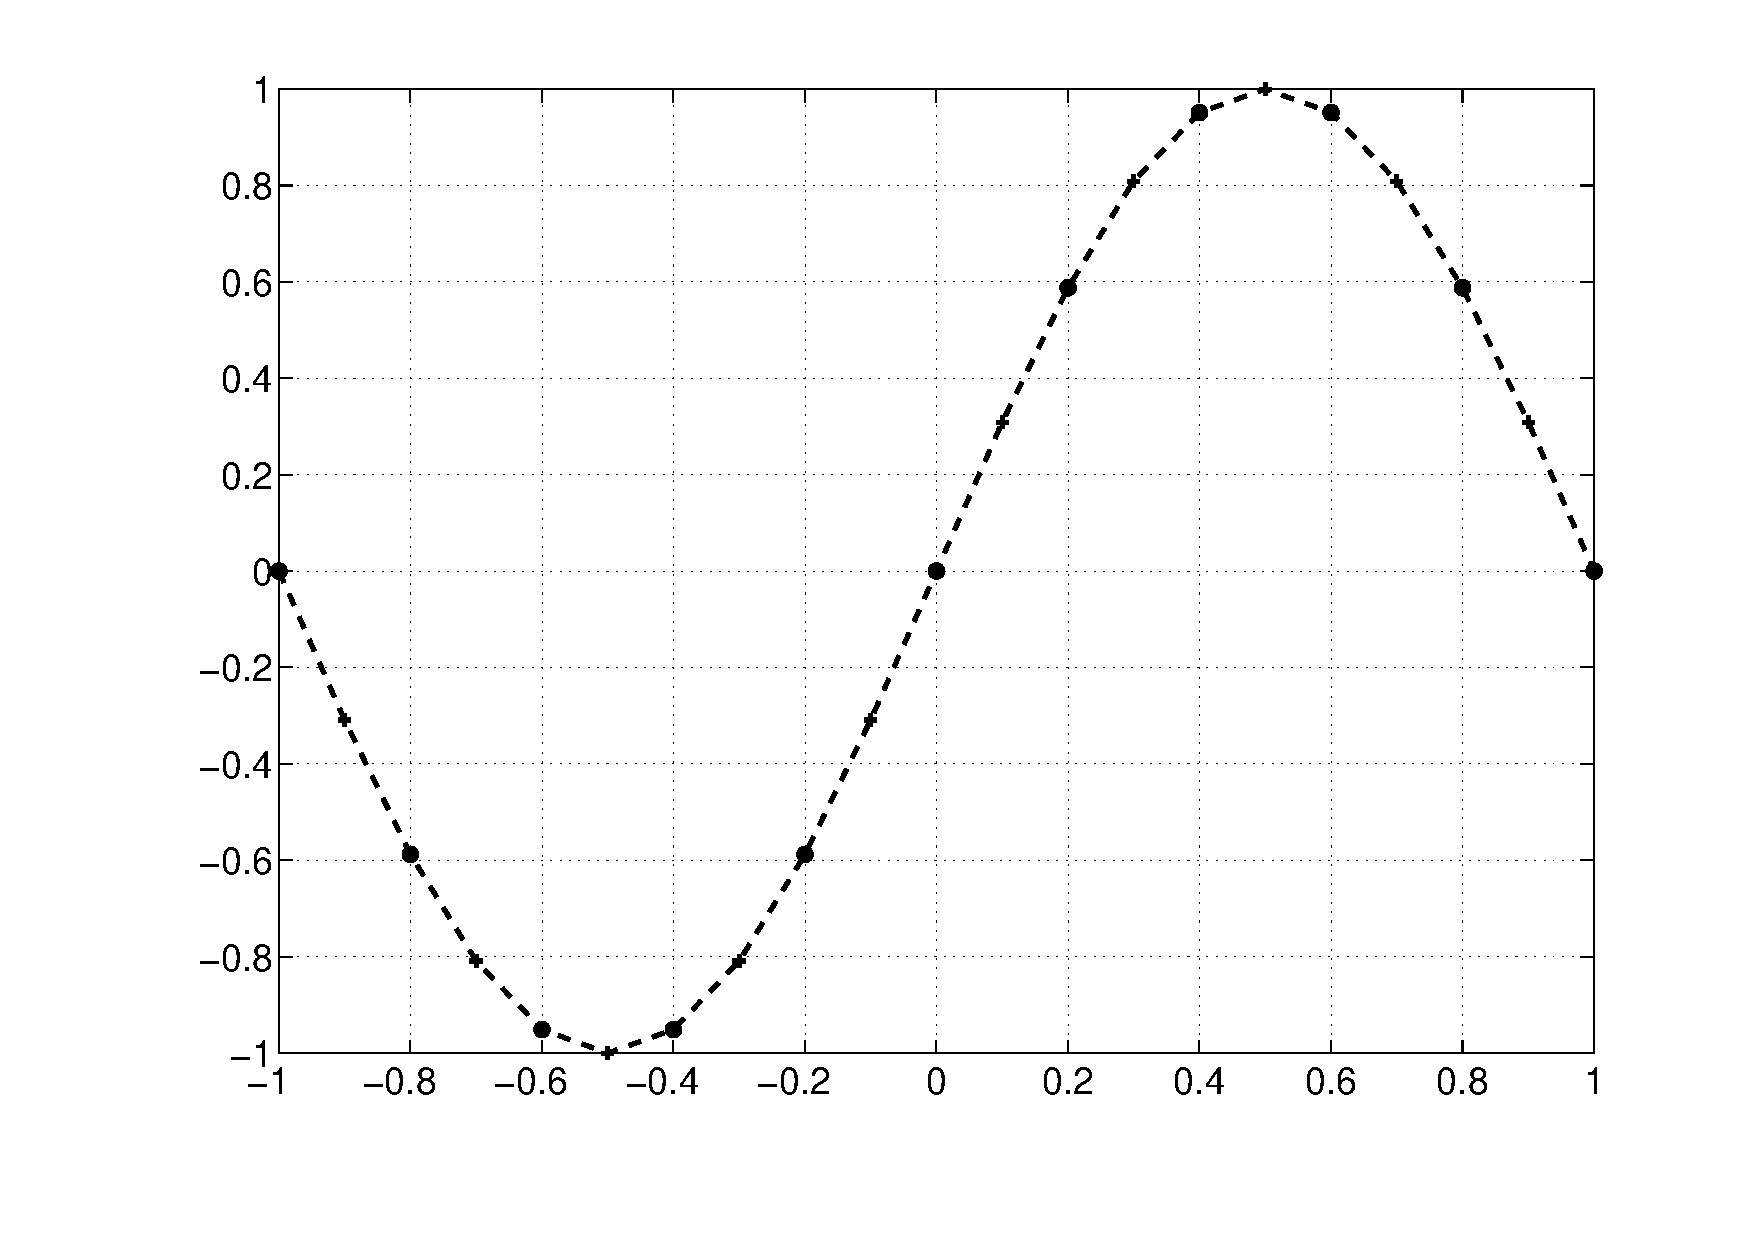
\includegraphics[scale=0.3, trim = 20mm 0mm 0mm 0mm, clip]{./Figures/1-HOFD/u_u.pdf}
\caption{$f(x)= sin(\pi x)$, uniform mesh. }
\end{figure}

\columnbreak

\begin{figure}[H]
\centering
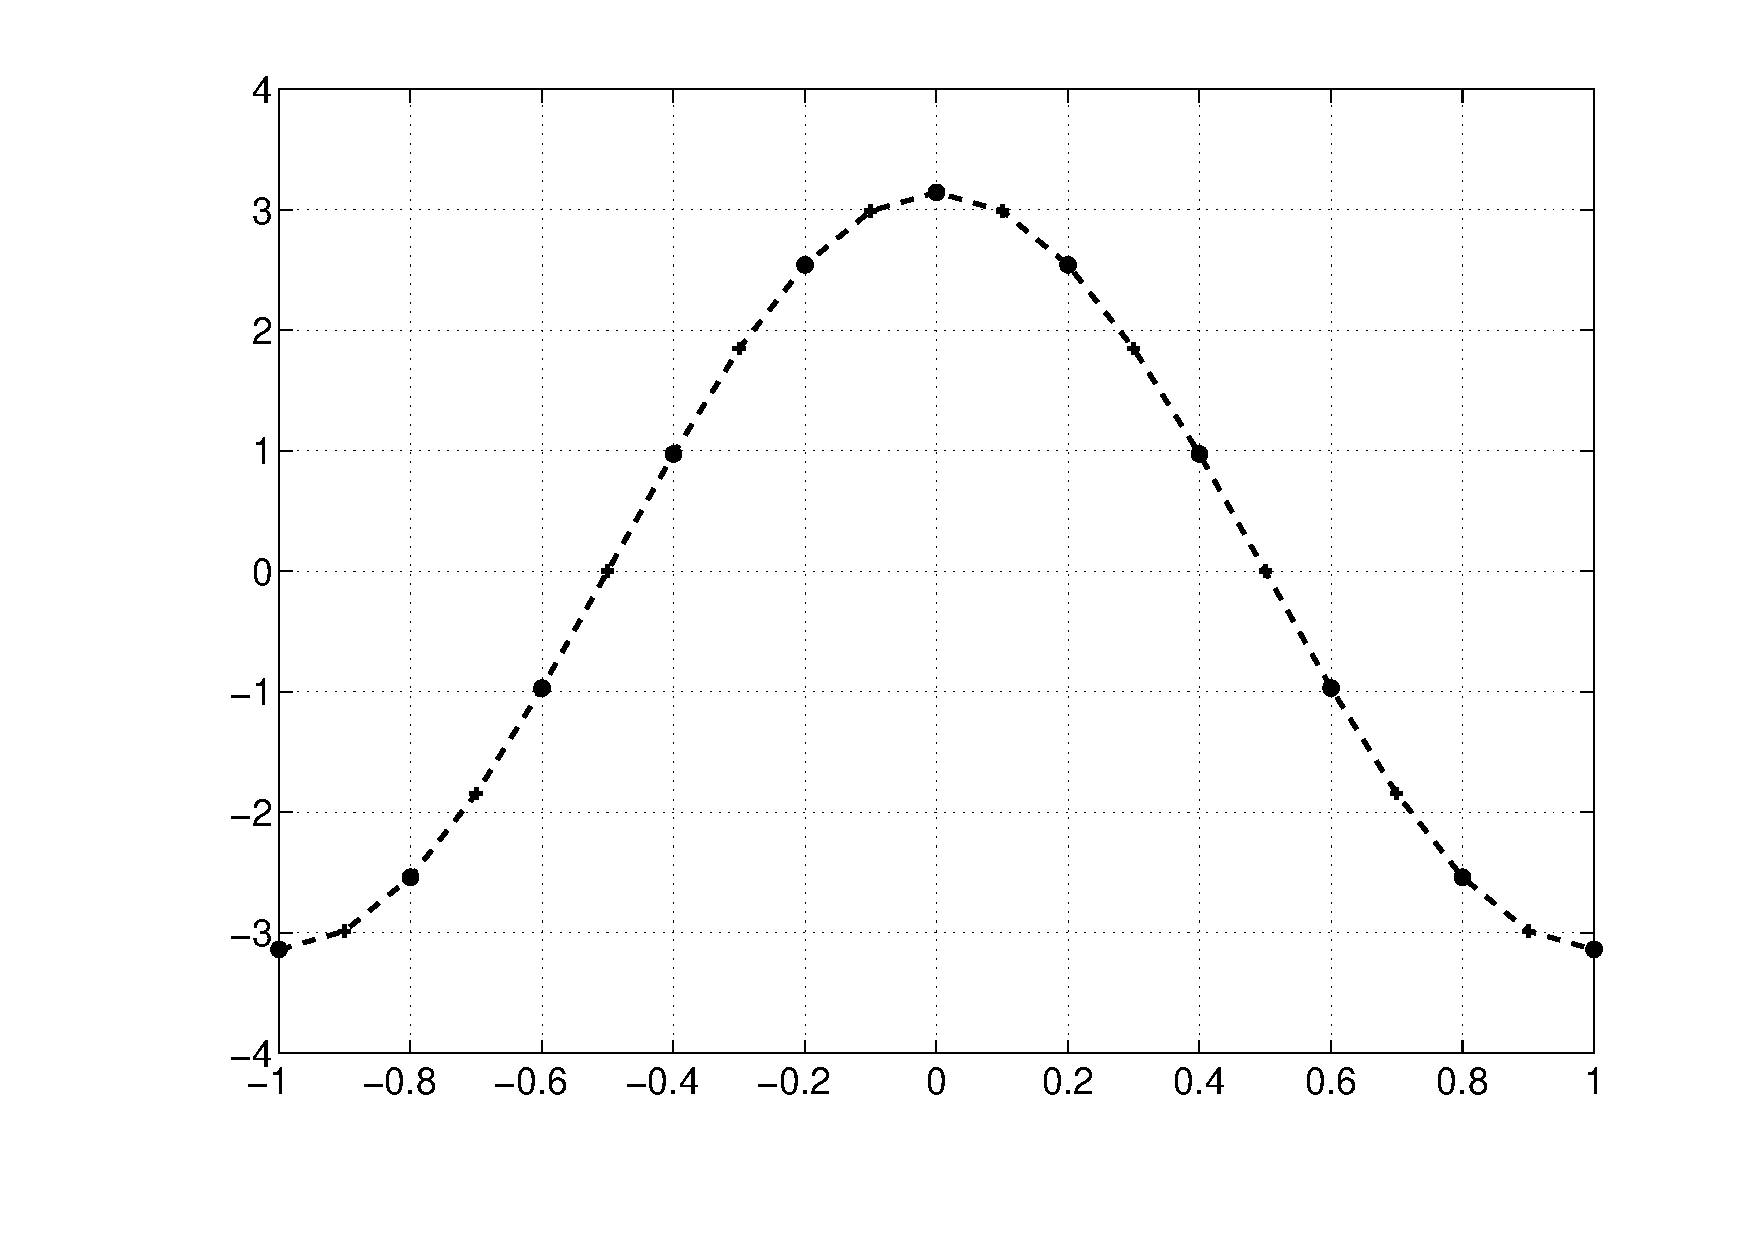
\includegraphics[scale=0.3, trim = 20mm 0mm 0mm 0mm, clip]{./Figures/1-HOFD/du_u.pdf}
\caption{$f'(x)$, uniform mesh. }
\end{figure}

\columnbreak

\begin{figure}[H]
\centering
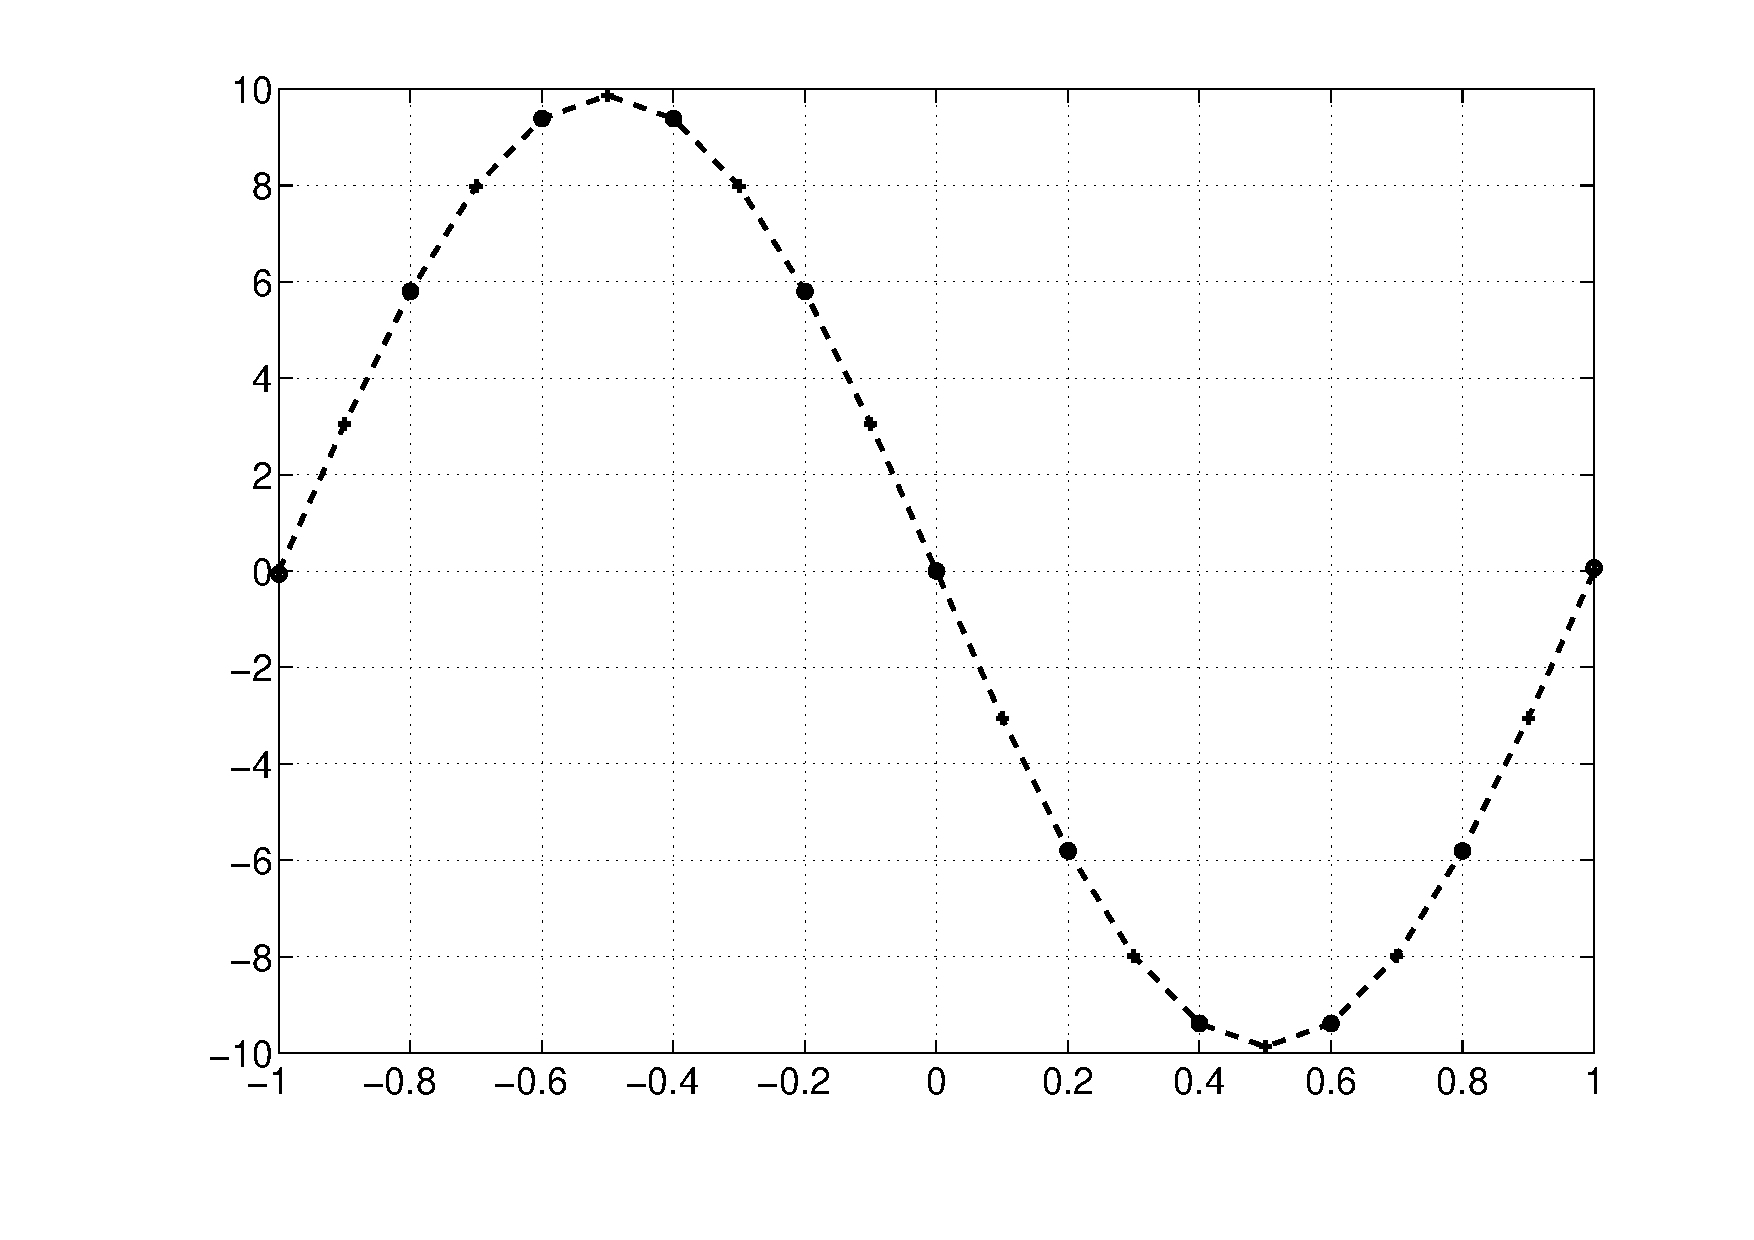
\includegraphics[scale=0.3, trim = 20mm 0mm 0mm 0mm, clip]{./Figures/1-HOFD/ddu_u.pdf}
\caption{$f''(x)$, uniform mesh. }
\end{figure}

\end{multicols}

\begin{multicols}{3}

\begin{figure}[H]
\centering
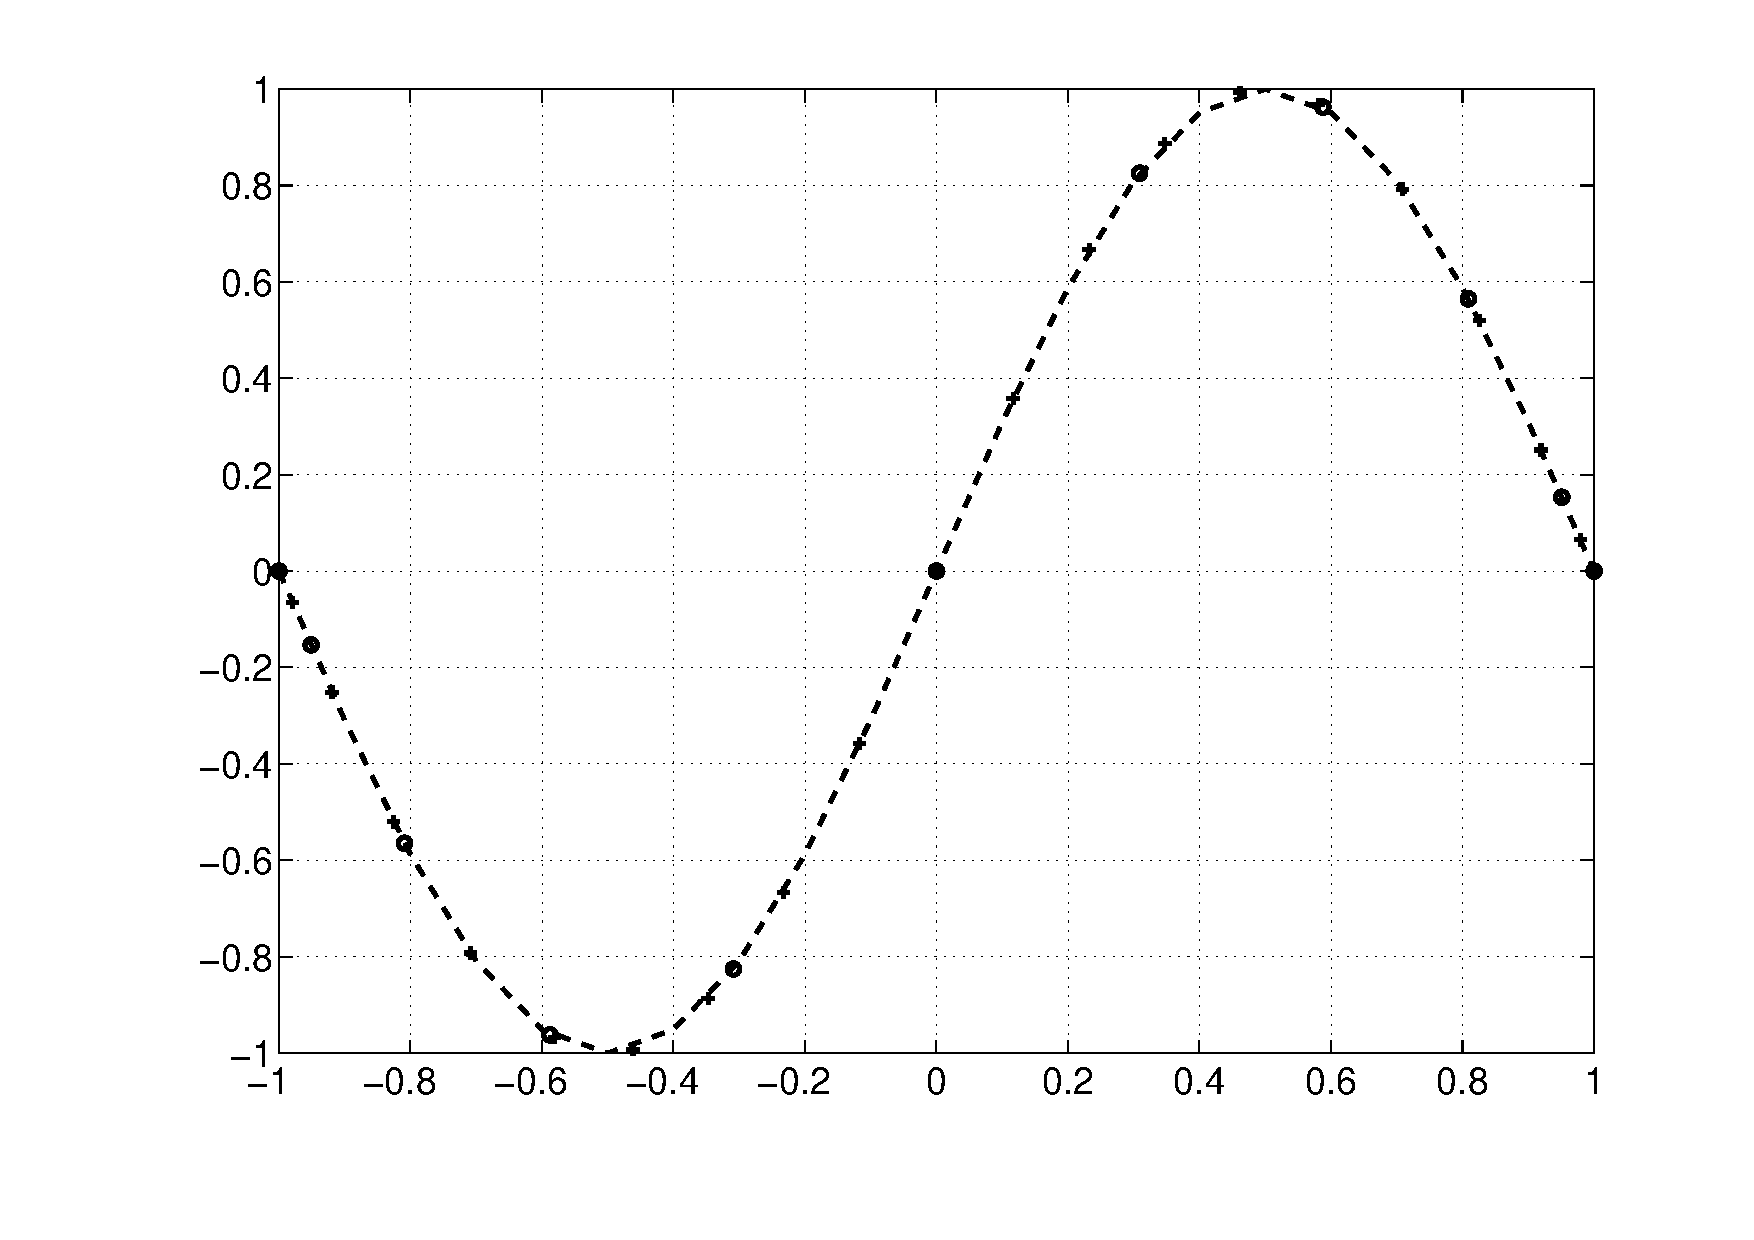
\includegraphics[scale=0.3, trim = 20mm 0mm 0mm 0mm, clip]{./Figures/1-HOFD/u_nonu.pdf}
\caption{$f(x)= sin(\pi x)$, non uniform mesh. }
\end{figure}

\columnbreak

\begin{figure}[H]
\centering
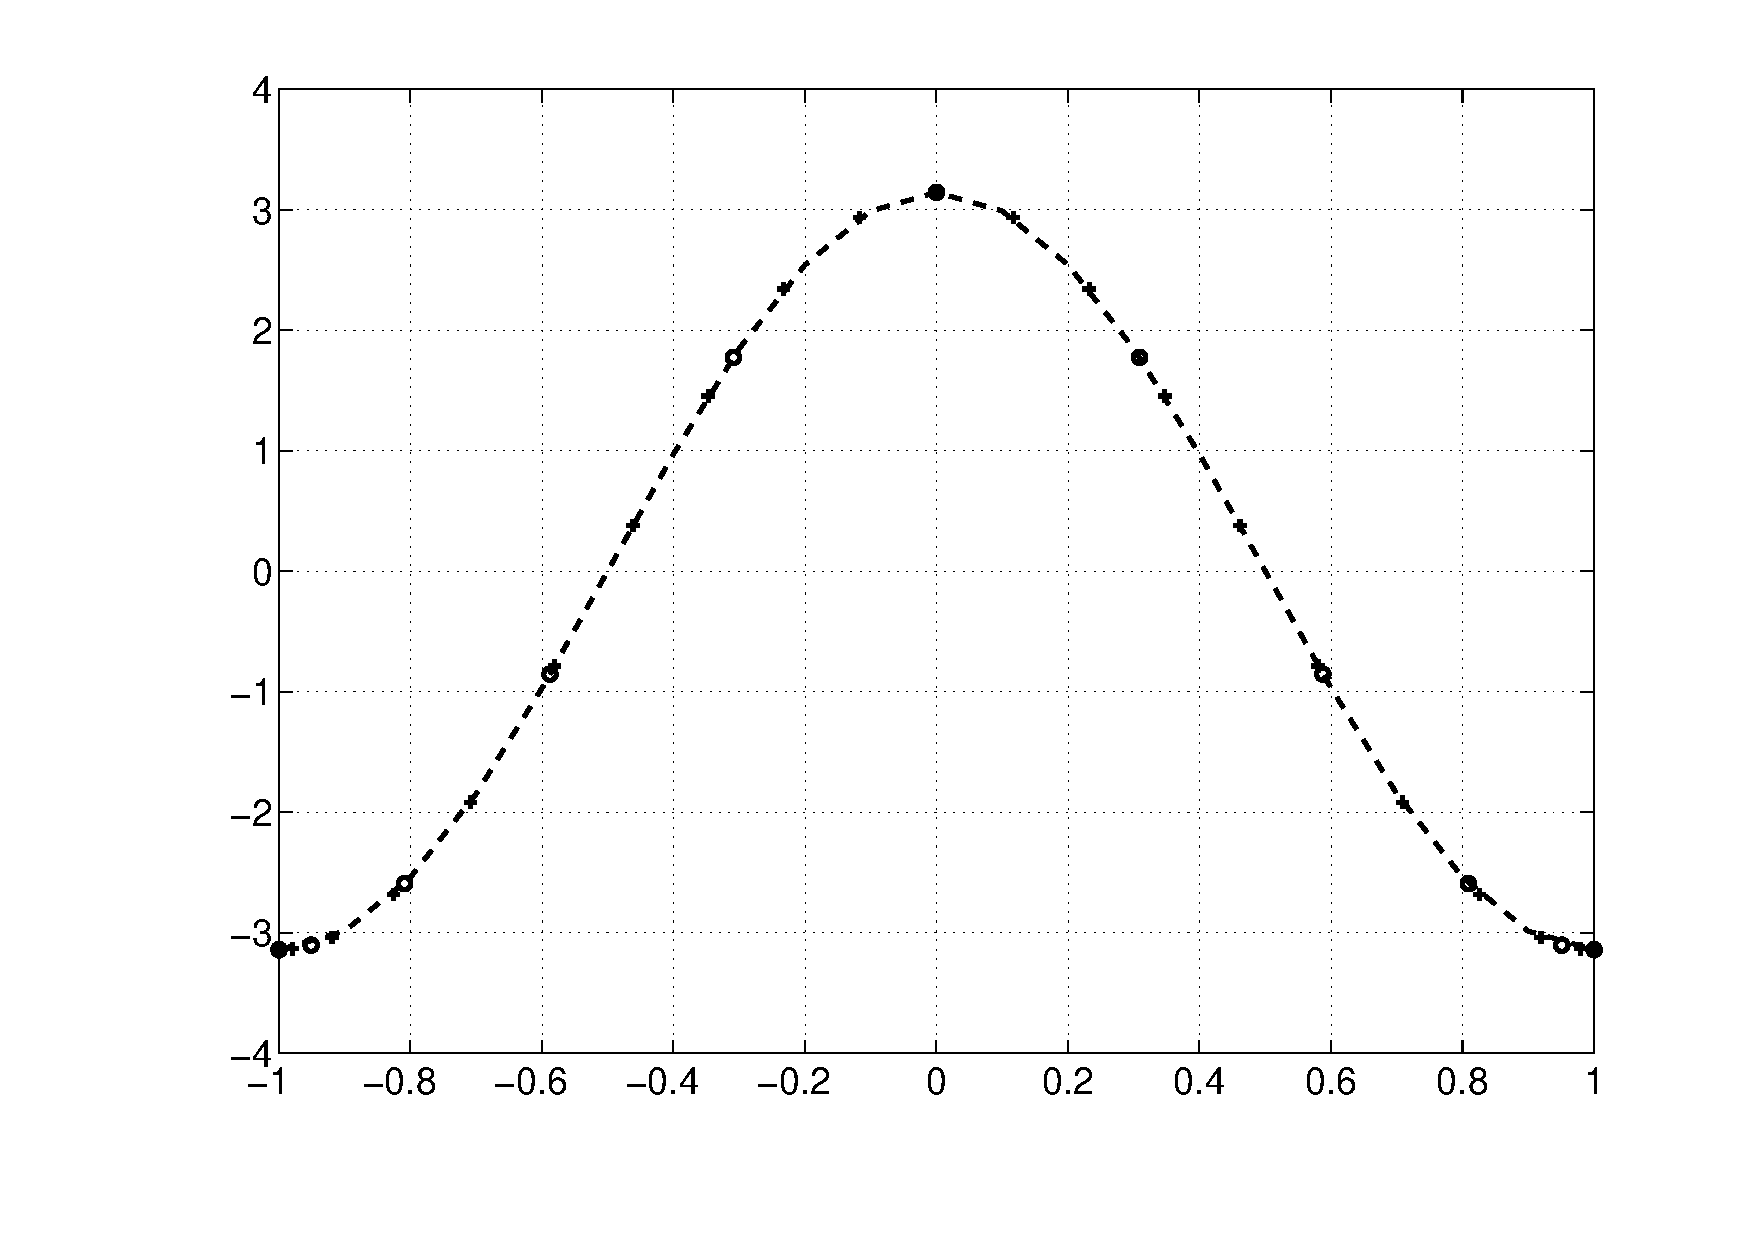
\includegraphics[scale=0.3, trim = 20mm 0mm 0mm 0mm, clip]{./Figures/1-HOFD/du_nonu.pdf}
\caption{$f'(x)$, non uniform mesh. }
\end{figure}

\columnbreak

\begin{figure}[H]
\centering
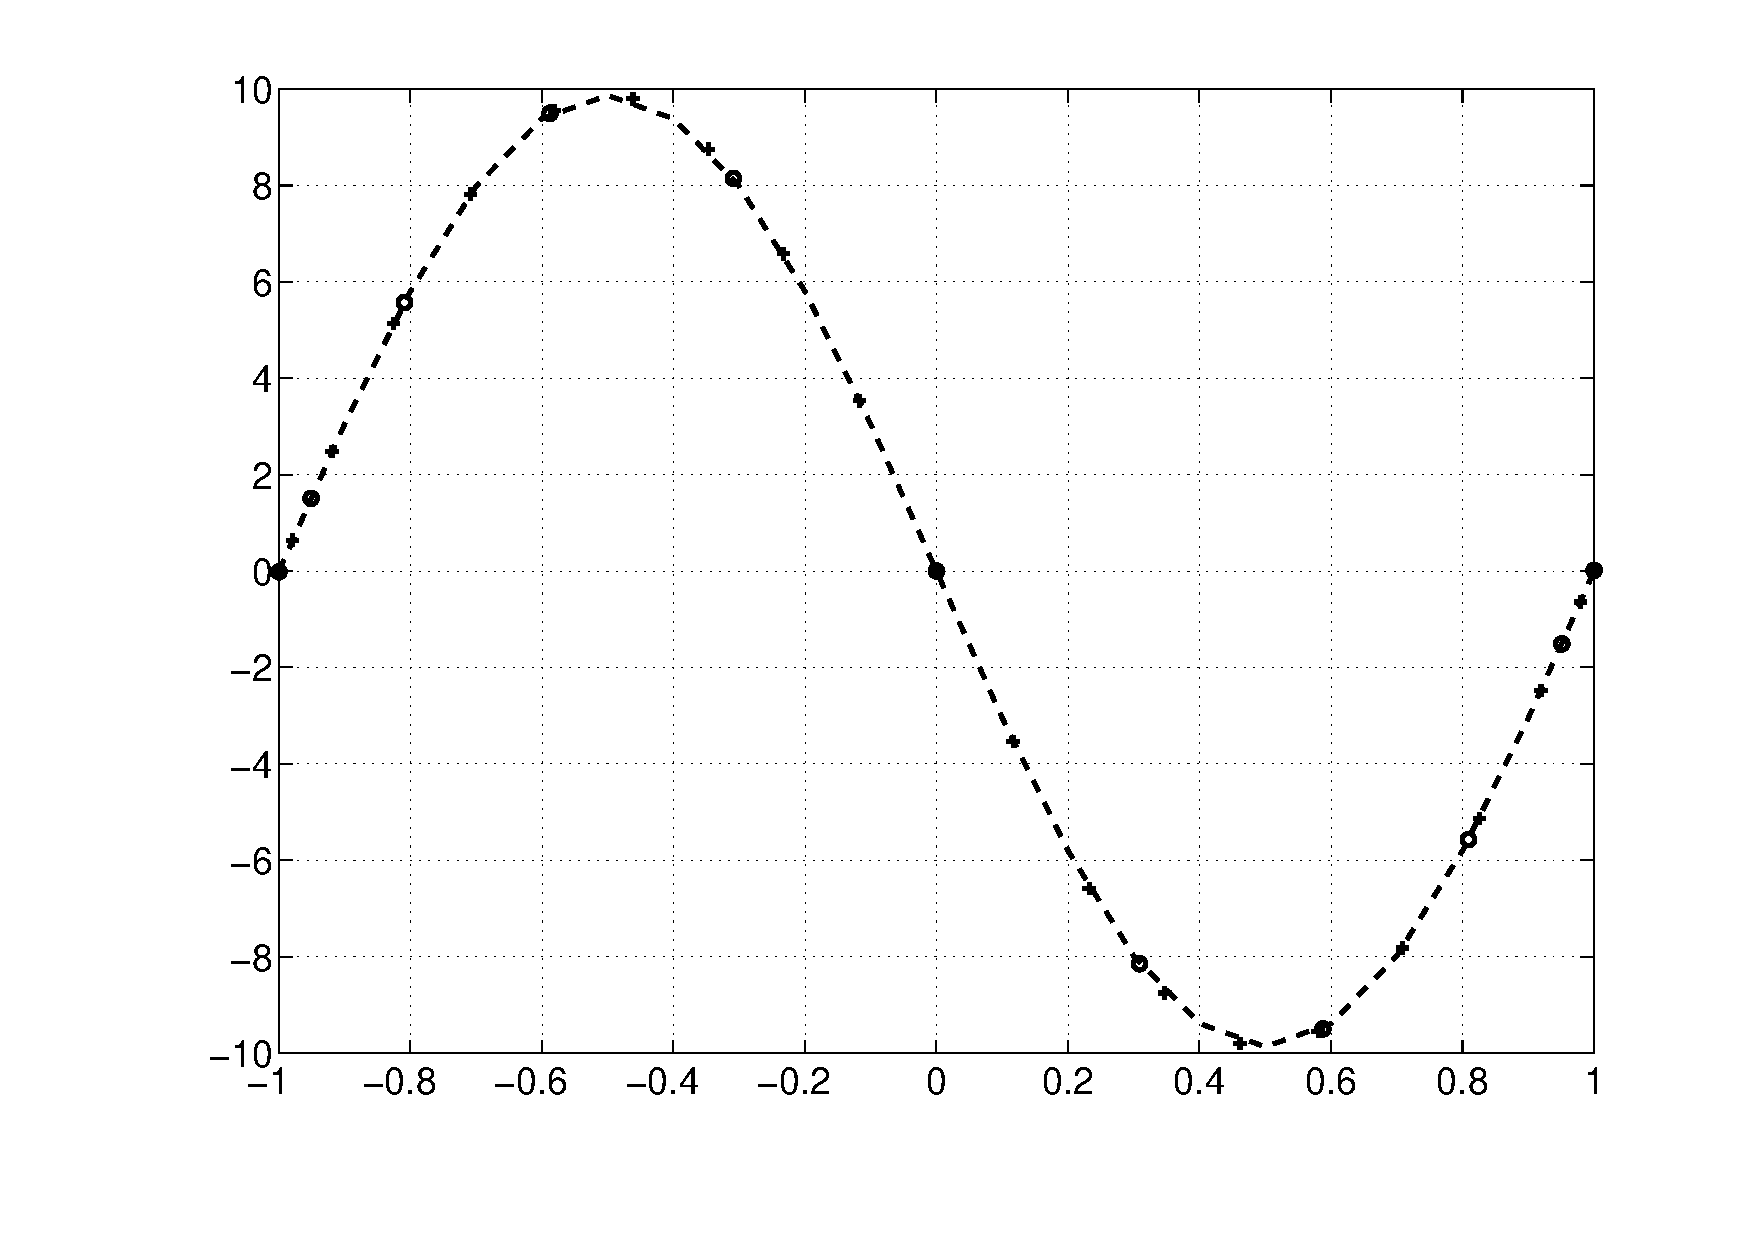
\includegraphics[scale=0.3, trim = 20mm 0mm 0mm 0mm, clip]{./Figures/1-HOFD/ddu_nonu.pdf}
\caption{$f''(x)$, nonuniform mesh. }
\end{figure}

\end{multicols}
\end{landscape}
\newpage

As we can see, the results are very accurate both using uniform and nonuniform
meshes. In the following figures the errors of the second derivative ($error=
u''_{exact}-u''_j$) are plotted:

\begin{multicols}{2}

\begin{figure}[H]
\centering
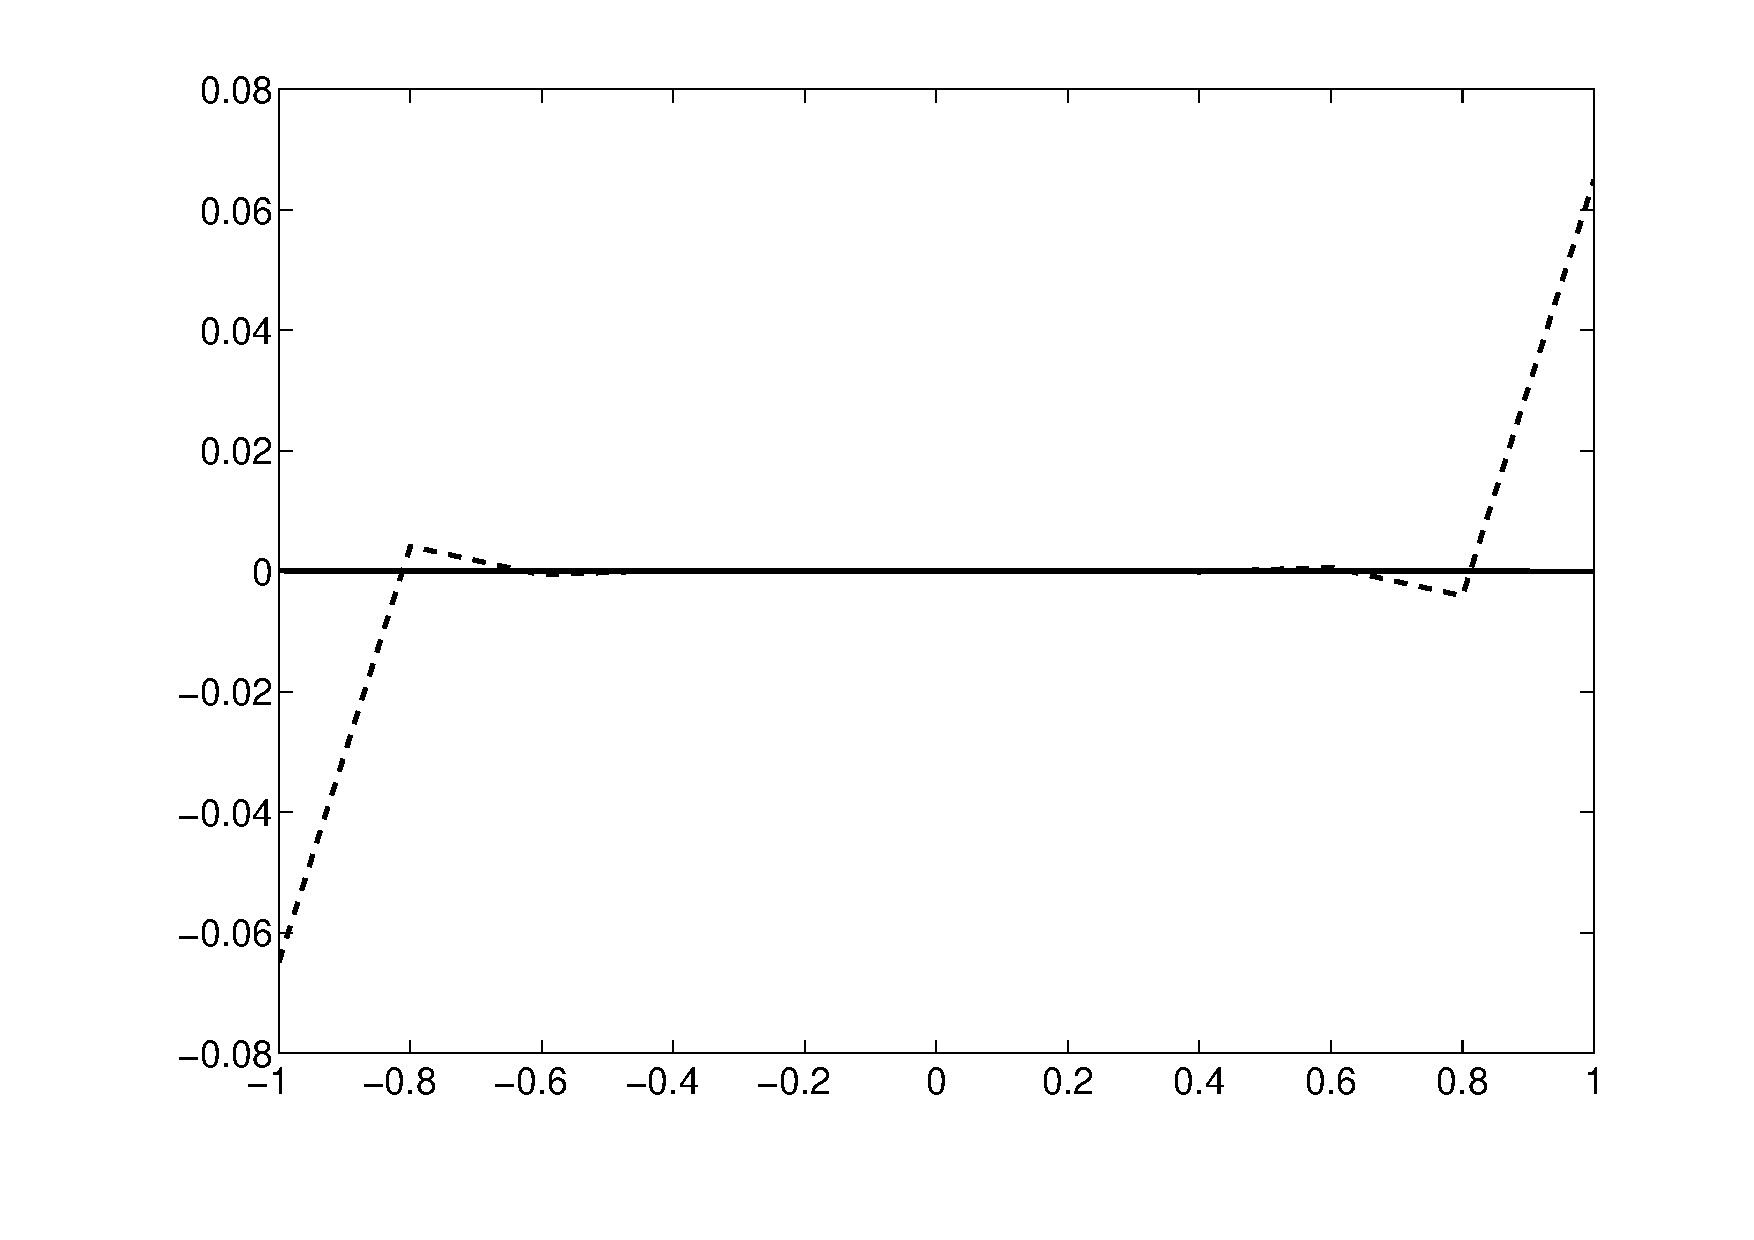
\includegraphics[scale=0.3, trim = 20mm 0mm 0mm 0mm, clip]
{./Figures/1-HOFD/error1.pdf}  \caption{Error of the uniform mesh using 10
(dashed) and 20 points (solid line).}
\end{figure}



\columnbreak

\begin{figure}[H]
\centering
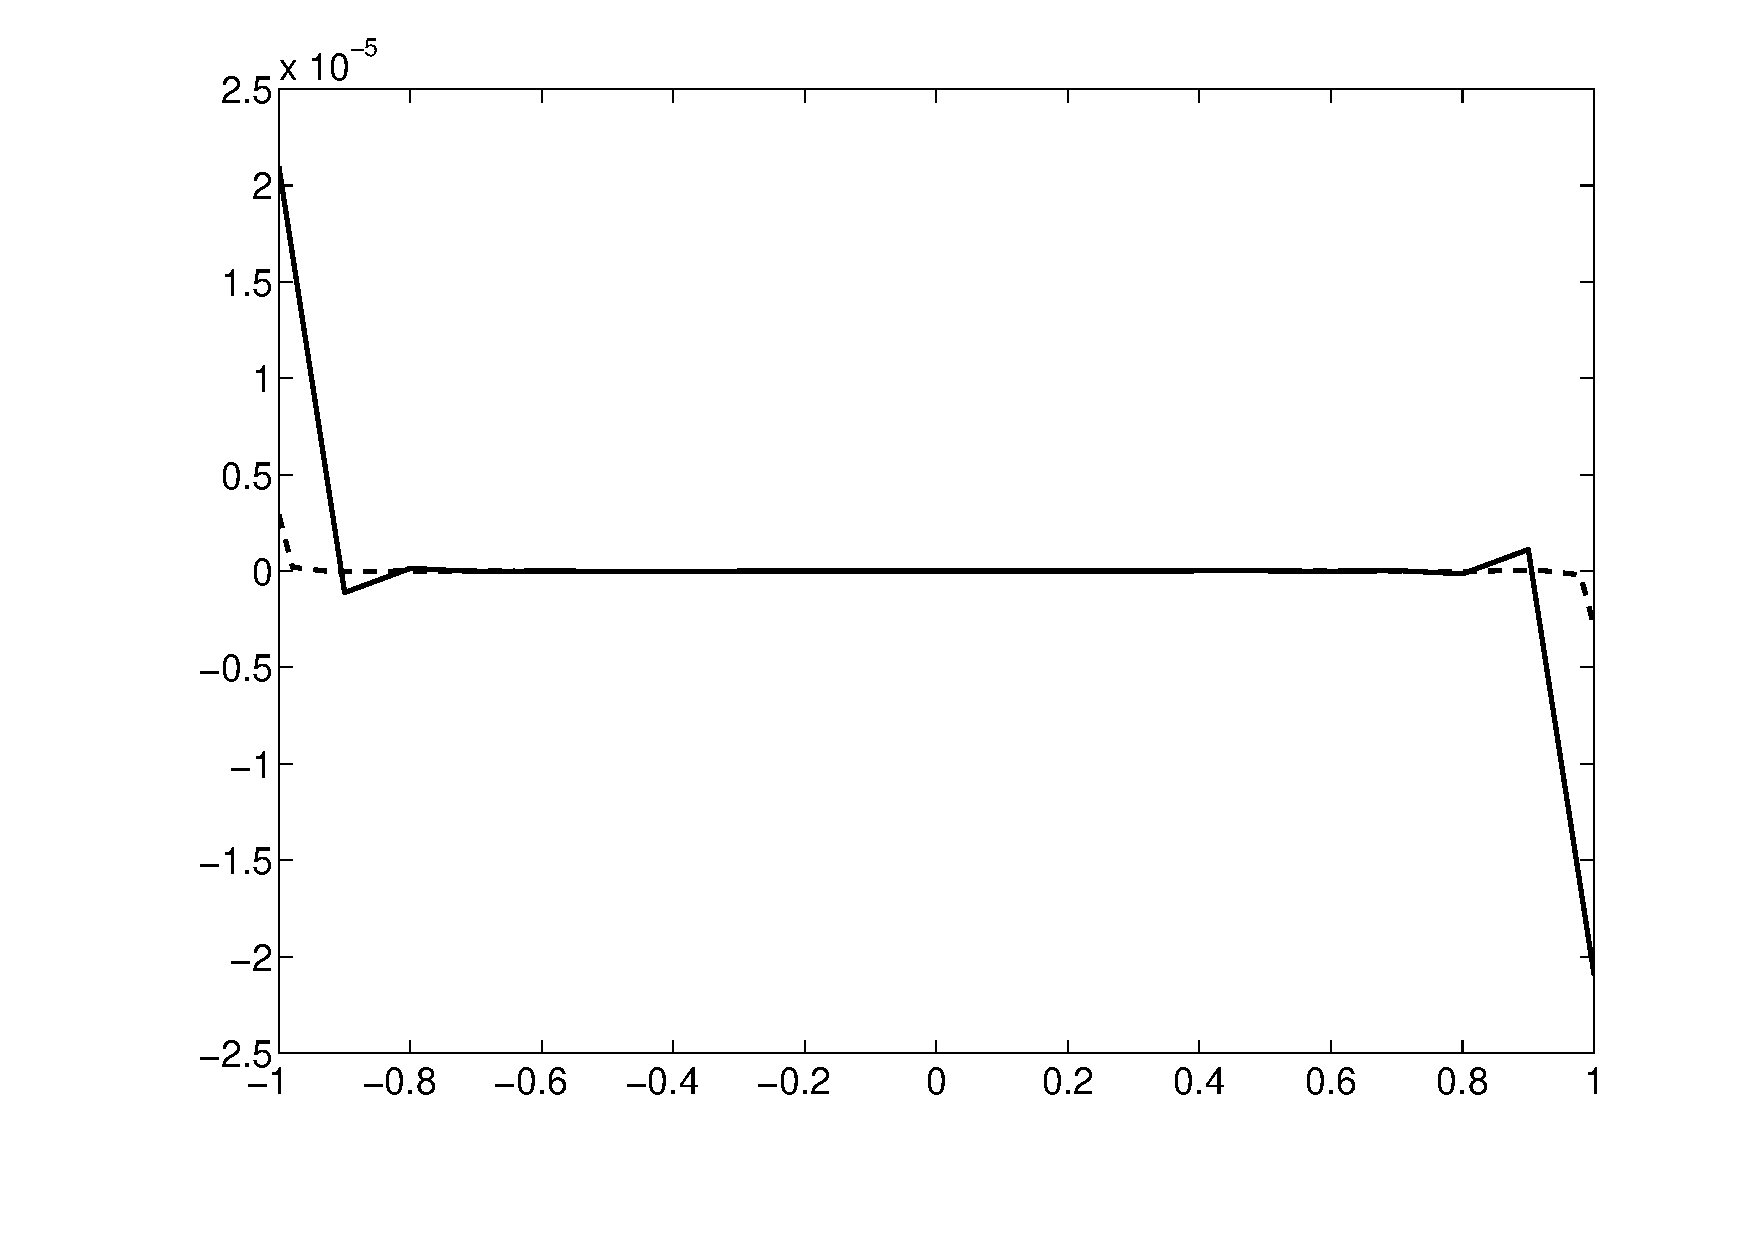
\includegraphics[scale=0.3, trim = 20mm 0mm 0mm 0mm, clip]{./Figures/1-HOFD/error2.pdf}
\caption{Error of the uniform mesh (solid line) and non uniform (dashed) using
20 points.}
\end{figure}

\end{multicols}

Besides the simplicity of this test case, we can see that the results obtained
are very good. Thus, we can extrapolate the functioning of this module to further applications. \\

\vspace{1cm}

In fact,  this program is able to calculate the derivatives of any
given 1D function $U=f(x)$ just changing the function definition line. The implications of this
simple method for such a complex procedure are many: 
\begin{itemize}
  \item The complexity is \textit{inside} the library. All that is seen from the
  API are some inputs and outputs arguments. 
  \item The syntax must be clear. In order to use the library, some rules must
  be regarded (in this case, the appropriate construction and arguments of the
  function \textit{Derivative}).
  \item The very same function is used for $x$ and $y$ derivatives, just
  changing the first input argument (\textit{Direction}).
\end{itemize}

The next example presents a 2D function. The idea is to show that the operations
are the same.\\

\newpage


\subsection{Laplacian of a function}
\label{laplacian}
% the \\ insures the section title is centered below the phrase: AppendixA
\begin{blueframed}
\begin{lstlisting}
program Laplacian

	use dislin
	use Finite_differences
	implicit none
	
	
  	integer, parameter :: N_x= 50, N_y= 50;!number of points
  	real ::  x(0:N_x), y(0:N_y)
	real:: U(0:N_x, 0:N_y)
	real:: Uxx(0:N_x, 0:N_y), Uyy(0:N_x, 0:N_y)
	real:: L(0:N_x, 0:N_y)
	integer :: Order = 20	!order of the interpolation
	integer :: i,j

	call Grid_Initialization( "uniform", "x", Order, x )
	call Grid_Initialization( "uniform", "y", Order, y )
	
	
	
	!function U=f(x,y)
	
	forall(i=0:N_x) U(i,:)=x(i)*x(i)+y*y ! an easy example
	
	 call Derivative( "x", 2, U, Uxx) 
	 call Derivative( "y", 2, U, Uyy) 

	 L=Uxx+Uyy
	 
	 ! Outputs (optional)
	  call scrmod('revers') 
	  call qplcon( L, N_x+1, N_y+1, 20);

end program
\end{lstlisting}
\end{blueframed}

The power of this library is clear with this example. Usually, computing the
\wk{Laplacian} of a function will involve a bunch of operations and a lot of
lines in our program. However, right now just one line is needed: $L=U_{xx}+U_{yy}$.\\

This procedure saves plenty of code lines with do-loops and complex
operations. The function assignment is written directly.\\

The next example continues with the higher complexity scale. The idea is to
prepare a program to perform the spatial discretization of the heat 1D
equation.\\

\newpage
\subsection{Heat equation (1D)}


We are going to deal with the following problem:

$$
\rho c_p \frac{\delta u}{\delta t}= k \frac{\delta^2 u}{\delta x^2};\;\;\;
+IC; \;\;\; +BC
$$

As we can see, this problem involves time and space. For now, we are just
interested in the \wk{spatial discretization}, so we are going to present the
operations for this purpose.\\

The idea is to transform the problem into something like: 

$$
\frac{\delta u}{\delta t}= \frac{k}{\rho c_p} \frac{\delta^2 u}{\delta
x^2};\;\Longrightarrow \frac{dU}{dt}= F(U,t)
$$

Also, the \wk{boundary conditions} must be discretized. Let's picture that the
boundary conditions are $u=T_0$ in $x=x_0$ and $\frac{\delta u}{\delta x}=0$ in $x=x_N$.\\

This is the example code for this application:

\begin{blueframed}
\begin{lstlisting}
subroutine heat_equation(t,U,F)

	real, intent(in) :: t
	real, intent(inout) :: U(:)
	real, intent(out) :: F(:)

	real :: alpha= 1., T0=1.
	real :: Uxx(0:Nx)
	
	integer:: Nx
	
	!Boundary conditions
	call Dirichlet ("x", 0, U, T0)
	call Newmann ("x", Nx, U, 0.0)

	!equation
	call Derivative("x",2,U,Uxx)
	
	F=alpha*Uxx
	
end subroutine
	
		
	
\end{lstlisting}
\end{blueframed}

Please, note that the program is not complete. There are some arguments that
have been supposed as knowns and some operations must be done before (meshing,
for example). Another module for the temporal discretization is needed in order to
solve the problem. However, the idea of this example is not to solve the
problem but to show the simplicity of the construction. The equation is written
the same way as it was when defining the problem:

$$
F(U,t)=\frac{k}{\rho c_p} \frac{\delta^2 u}{\delta
x^2} \Longrightarrow F=alpha*Uxx
$$






%%\end{document}


\newpage
\chapter{Cauchy Problem}

The aim of this paper is to serve as a manual for using the software application
given. With the aid of this manual, the reader should be prepared for solving
initial condition problems using high-order finite-difference schemes.\\

A whole and precise description of the subroutines and procedures joined under
the program structure is beyond the bounds of this work. The purpose of this text is
to familiarise the reader with the numerical approach to these problems and to
give the essential information in order to use the software.  \\

The most part of the effort will be dedicated to the description of the
\underline{application programming interface} of this software. An API is an
ensemble of procedures and subroutines which determines how a piece of the program interacts
with an other.  \\

After the read of this paper the user will understand the first
layer of the program, and will be able to write his/her problems
according to the API's structure. 



%1.==========================BODY==============================================
\newpage

\section{Introduction}

An initial-boundary value problem is one of the most generic structures in
mathematics. It can involve both temporal and spatial derivatives. Generally
speaking, we may find something in the shape of: 

\begin{Large}
$$\begin{cases} \frac{d \mathbf{U}}{dt}=   {\mathscr{L}}( \mathbf U,
	t, \mathbf x) \\[0.25cm]
	\hspace {0.25cm}+ IC \quad + BC
	\end{cases}$$
\end{Large}
\\

Where the $\mathscr{L}$ includes any mathematical operator, so the problem can
be an ordinary differential equation (\textit{ODE}) and also a partial
differential equation (\textit{PDE}). \\

The method for the numerical resolution of this problem involves the
transformation of the problem to an easier structure. \\

First of all the general problem should be reduced to an ODE. Usually, this step
involves the \underline{spatial discretization} of the problem. Once this
operations are finished, the equations should have the following structure: 


	$$\begin{cases} \frac{d \mathbf{U}}{dt}=  \mathbf F( \mathbf U, t)  \\[0.25cm]
	\hspace {0.25cm}+ IC 
	\end{cases}$$
	\\
	
This is known as \underline{Cauchy problem} in the mathematical bibliography.
There exist a huge collection of methods and procedures for solving problems
under this structure. The importance of this expression is that any
initial-boundary value problem can be reduced to this, so once the right part of
the assignment (the $\mathbf F( \mathbf U, t)$) is defined, the numerical
solution of the resulting equation implicates always the same steps. The idea of
the library is to hold the procedures so it can be launched for any given
problem.\\

The approach to the numerical solution of any given problem can be summarized in
the following chart: \\

\begin{framed}

\framebox[3cm]{\textbf{Physics}}% 
	\hfill
	\framebox[12cm]{\textbf{Mathematics}} \\
	
{\begin{small}	
	
\framebox[3cm]{$\begin{cases}\text{Equations}\\ 
+IC +BC\end{cases}$}%
$\: \Rightarrow  {\mathscr{L}}( \mathbf U,
	t, \mathbf x)\: \rightarrow$
\framebox[2.5cm]{$\begin{matrix} \text{Spatial}\\
\text{discretization}\end{matrix}$}%
$ \: \rightarrow \mathbf F( \mathbf U, t)\rightarrow$
\framebox[2.5cm]{$\begin{matrix} \text{Temporal}\\
\text{discretization}\end{matrix}$}
$\: \Longrightarrow \: \mathbf{U}(t)$

\end{small}}

\end{framed}

\vspace{1cm}

The idea of the software application is to hold the operations contined under
the label \textit{mathematics}. This way, the resolution of the problems will be
automatic, once the \textit{physics} are defined. \\

The advantage of proceding this way is that all the complex mathematical
operations are encapsulated inside the library \textbf{Cauchy\_Problem}, where
the routines and procedures have been carefully defined, tested and validated.
All the operations are structured in layers, and the effort of the user
is reduced to the definition of the higher one: the \underline{Application
Layer}, where the problem should be written according to the \textbf{API} of
the layers underneath.\\

The purpose of this manual is to help with the construction of the application layer, according to the specific rules and
procedures that the API fixes. \\

So, the software application has the following structure: \\

\begin{framed}

\begin{framed}
\centering 
{\Large \textbf{Application layer}}


\end{framed}

\begin{multicols}{2}
\centering
$\Uparrow \:API_{HOFD}\: \Downarrow$

\begin{framed}

\textbf{Spatial semi-discretization}

\begin{multicols}{2}
\begin{framed}
Grids\\
\end{framed}

\columnbreak

\begin{framed}
{{Finite\\ differences}}
\end{framed}

\end{multicols}

\begin{framed}
Lagrange interpolation
\end{framed}

\end{framed}

\centering
$\Uparrow \:\: \Downarrow$

\columnbreak 

\centering
$\Uparrow \:API_{Cauchy Problem}\: \Downarrow$

\begin{framed}
\textbf{Temporal semi-discretization}

\begin{framed}
Cauchy Problem
\end{framed}
\vspace{0.3cm}

\begin{framed}
Temporal schemes\\
\end{framed}

\end{framed}
\centering
$\Uparrow \:\: \Downarrow$


\end{multicols}

\begin{framed}
\centering Numerical recipes (linear/non linear algebra)
\end{framed}

\end{framed}

Where \underline{only the application layer} is to be changed, while all the
other modules are encapsulated inside the library. \\

%==================================

\newpage
\subsection{Examples of application}

In this section we are going to deal with three different problems in a higher
complexity scale. We will see how the problem can be transformed to something
in the shape of what he have been talking about.\\

 First of all, an ODEs problem is presented, the well-known
mass-spring-damper system. The advantage of this problem is that we will not
need the spatial discretization, since spatial derivatives are not included in
the problem's definition.\\

Then we will deal with Lorenz attractor. This is also an ODEs problem, this
time involving multiple dimensions.\\

Finally we will reach an intial value PDEs problem, whose numerical
resolution procedure involves all the actions we have described in this
section. \footnote{go to the appendices to check the software implementation
of these problems.}\\

\subsubsection*{Mass-spring-damper system}

The following problem is considered:
$$
M \ddot x + D \dot x + K x = P(t)
$$

With the initial conditions: 
$$
x(t=0)=x_0; \;\;\; \dot x (t=0)= \dot x_0
$$\\

First of all, the problem must be transformed into a first order derivative
(Cauchy problem structure).

For this purpose, a vector of unknown variables is defined:
$$
U=[x,  \dot x] \Longrightarrow \frac{d \mathbf{U}}{dt}= \mathbf{F}(\mathbf{U},t)
$$
$$
\frac{d}{dt}\begin{bmatrix}
U(1)\\
U(2)
\end{bmatrix}= 
\begin{bmatrix}
F(1)\\
F(2)
\end{bmatrix}
\Longrightarrow \mathbf{F}=\begin{bmatrix}
U(2)\\
\frac{1}{M}\cdot (P(t)-D\cdot U(2)-K \cdot U(1))
\end{bmatrix} 
$$\\

This function $F=F(U)$ is going to be named \underline{system} in the software
application.
As we can see, even in a simple example is a vector function.\\

Now that the Cauchy problem is defined, the program is able to continue with the
numerical resolution. Here, some opetions must be chosen (numerical scheme,
duration, time steps\ldots). For the shake of simplicity let's assume we want to
use an explicit Euler scheme:\\

\begin{framed}
$$
n=0,\;\; t=t_0, \;\; \mathbf{U}^0=[x_0, \dot x_0]
$$

\begin{framed}
$n \rightarrow$ \framebox[5cm]{$\mathbf{F}^n=\mathbf{F} (\mathbf{U}^{n})$}% 
	$\rightarrow$
	\framebox[5cm]{$\mathbf{U}^{n+1}=\mathbf{U}^n + \Delta t \cdot \mathbf{F}^n$}% 
	$\rightarrow$
	$\mathbf{U}^{n+1}$ \\
	$$\longleftarrow n=n+1 \longleftarrow$$
\end{framed}

\end{framed}

\subsubsection*{Lorenz attractor}

Now we are going to consider the following problem: 
{\large{
$$
\begin{cases}
\frac{dx}{dt}= a \cdot ( y - x ) \\
\frac{dy}{dt} =x \cdot ( b - z ) - y \\ 
\frac{dz}{dt} =x \cdot y - c \cdot z \\
\end{cases}
$$
}}
$$
x(t=0)=x_0;\;\; y(t=0)=y_0;\;\; y(t=0)=y_0
$$\\

As we can see, this is already a first order derivative problem. So, the
transformation is inmediate: 
$$
\mathbf{U}=[x,y,z] \longrightarrow \frac{d}{dt} \begin{bmatrix}
U(1)\\
U(2)\\
U(3)
\end{bmatrix}= 
\begin{bmatrix}
a \cdot ( U(2) - U(1) ) \\
U(1) \cdot ( b - U(3) ) - U(2) \\ 
U(1) \cdot U(2) - c \cdot U(3) \\
\end{bmatrix}=\begin{bmatrix}
F(1)\\
F(2)\\
F(3)
\end{bmatrix}
$$\\

The connection with the previous problem is evident, 
$$
\frac{d \mathbf{U}}{dt}= \mathbf{F}(\mathbf{U},t)
$$

Therefore, we can think of a first extrapolation: once we arrive to a
\textbf{Cauchy problem}, \underline{the solving procedure is the same}.\\

\newpage
If we assume we have a solver for this type of problems, the input arguments to
this program should be something like: \\

\begin{framed}
\textbf{Cauchy problem} \\

\hspace{1cm} Initial conditions ($\mathbf{U}^0$)

\hspace{1cm} System ($\mathbf{F}(\mathbf{U},t)$)

\hspace{1cm} Temporal scheme (Explicit Euler in the previous example)

\hspace{1cm} Time iteration ($n$)
\end{framed}

\vspace{1 cm}

With this structure both the previous (mass-spring-damper) and this program
(lorenz attractor) can be solved.\\

The importance of this structure is that the same piece of code will be useful
for solving a huge amount of problems, so a great deal of time and effort is
saved. Also, this method allows us to test the different modules separetely, in
order to assure its functionallity. Finally, but any less important, we can
change the resolution process (temporal scheme/time domain) with little effort.
This might be decisive when dealing with stability matters. \\

\newpage

Now, let's look how the Cauchy problem is written in the program: \\

\begin{blueframed}
{\small
\begin{lstlisting}
subroutine Cauchy_Problem_Solution( Domain,  Initial_C, System, 
				Scheme, Outputs) 
        
     procedure (Temporal_Domain)  :: Domain 
     procedure (Initial_Condition) :: Initial_C
     procedure (System_ODES) :: System
     procedure (Temporal_Scheme), optional :: Scheme
     procedure (ODES_Outputs), optional :: Outputs 
     
     ![...]
\end{lstlisting}
}
\end{blueframed}

\vspace{0.5cm}

We can see that this is pretty much the very same structure that the one shown
in the conceptual construction.\\

The subroutine needs the input arguments of time, system and initial conditions. The temporal
scheme is declared as optional: if there is not an specific choice, the program
will continue with the default procedure (Runge-Kutta RK4).
\\

The subroutine also includes another procedure which is used to extract
information from the resolution process (${ODES\_ Outputs}$), but it is
not necessary for the program to run (it has the label \textit{optional}).\\

Summarizing for fixing ideas: when dealing with problems, we are not
interested in developing a specific software for each equation. It is much
more efficient to generate a procedure which can be used equally for different
problems (\textit{interchangeability}).\\

With this two examples, we have seen how two different problems are solved with 
the same routine. Although the problems
were simple, the idea behind these examples is very powerful; and it will be
demonstrated with the next problem, which involves also spatial
discretization.\\

\subsubsection*{Heat equation 1D}

We are going to deal with the following problem:
$$
\rho \cdot c_p \frac{\delta u}{\delta t}= k \frac{\delta^2 u}{\delta x^2};\;\;\;
+IC; \;\;\; +BC
$$

The procedure for solving this equation can be divided in two groups of
operations as we have seen before: spatial semi-discretization and the
resulting Cauchy problem (as this problem is already a first-order derivative;
otherwise some other operations must be done).\\

\newpage
a) Spatial semi-discretization\\

\begin{figure}[h]
\centering
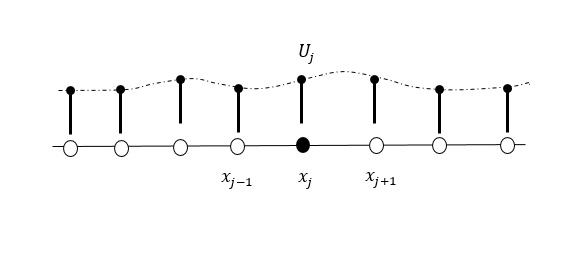
\includegraphics[scale=0.7, trim = 30mm 15mm 25mm 0mm,
clip]{./Figures/2-CauchyProblem/spatial_discretization.jpg}
\caption{Spatial discretization}
\end{figure}

$$
\frac{\delta u}{\delta t}= \frac{k}{\rho \cdot c_p } \frac{\delta^2 u}{\delta
x^2} \Longrightarrow \left(\frac{\delta^2 u}{\delta
x^2}\right)_{x=x_j} = f(U_{j-p},\ldots U_j \ldots U_{j+q})$$

$$
BC \Longrightarrow g(U_0,U_1,\ldots)=0;$$\\

For example, using equally-spaced second order interpolation, 
$$
x_j= a+(b-a) \cdot \frac{j}{m}; \;\;\; j\in [0,m]
$$
$$
\Delta x= x_j-x_{j-1}= \frac{b-a}{m}
$$

the spatial
discretization of the partial derivative $\frac{\delta^2 u}{\delta
x^2}$ will give: 

$$
\left(\frac{\delta^2 u}{\delta
x^2}\right)_{x=x_j} ={\Delta x^2} \cdot ( u_{j-1}
-2 \cdot u_{j} +u_{j+1}) \;\;\; j\in[1,(m-1)]$$\\

And assuming a boundary condition type Neumann at $x=a$ and type Dirichlet at
$x=b$, we have: 

$$
Neumann: \:\: \left(\frac{\delta u}{\delta
x}\right)_{x=a} =0; \Longrightarrow \frac{2}{\Delta
x}\cdot (3 \cdot u_0 -4 \cdot u_{1} + u_{2}) =0$$


$$
Dirichlet: \:\: u(x=b)=0; \Longrightarrow u_m=0
$$

\begin{figure}[h]
\centering
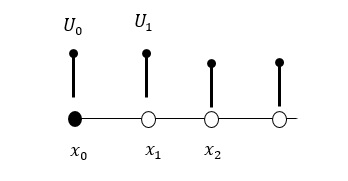
\includegraphics[scale=0.7, trim = 10mm 0mm 15mm 0mm,
clip]{./Figures/2-CauchyProblem/BC.jpg}
\caption{Boundary conditions}
\end{figure}

In a general way, any boundary condition can be written as: 
$$
F(u(x))=g;\;\; \text{if} \:\: x \in \delta\Omega \rightarrow u_0=f(u_1,u_2,
u_3,\ldots, g) $$

So, the problem has been transformed from a continuous function $u(x,t)$ to a
discrete distribution of values of this function $u_j(t)=u(x_j,t)$; which are
now the unknown quantities. Then, the problem has $m+1$ values to be
determined.\\

b) Cauchy problem \\

Once the spatial discretization is done we get a Cauchy problem: 

$$
\left(\frac{\delta u}{\delta t}\right)_j= \frac{k}{\rho \cdot c_p }\cdot {\Delta x^2} \cdot ( u_{j-1}
-2 \cdot u_{j} +u_{j+1})\\
$$

Or more generally, for any given interpolation order, $2p+1$: 

$$
\left(\frac{\delta u}{\delta t}\right)_j= f(u_{j-p},\ldots u_j, \ldots
u_{j+p})\\
$$

$$
+IC
$$

Where the unknown variables are the components of the vector $U=[U_0, U_1\ldots
, U_m]$. To continue from here, we can use the same routine as the one defined in the previous examples. \\


As we can see this process is not easy. However, using the appropriate software
tools the most part of the diffculty can be hidden. The combination of the
spatial discretization library \footnote{see High Order Finite Differences
manual (HOFD\_manual)} and the Cauchy Problem solver, complex problems can be
set to work.\\

\newpage

The process for solving a PDE problem can be summarized in the
following chart: \\

\begin{framed}
\textbf{\large PDE problem}\\
\small{

	\framebox[3.5cm]{Equations}% 
	$\rightarrow$
	\framebox[4cm]{Spatial \\ discretization}% 
	$\rightarrow$
	\framebox[1.8cm]{\textbf{System}} 
	$\iff$
	\framebox[3cm]{Cauchy problem}\\
	
	\framebox[3.5cm]{ $\begin{cases}
	\frac{d\mathbf U}{dt}={\mathscr{L}}( \mathbf U,
	t, \mathbf x)\\ 
	+IC; +BC
	\end{cases}$}% 
	$\rightarrow$
	\framebox[4cm]{ $ \begin{cases}
	 \mathbf{U}(x_j,t) \rightarrow u_j\\ 
	I_j = I_j (u_j, x) \end{cases}$}% 
	$\rightarrow$
	\framebox[1.8cm]{ $ \begin{cases}
	F(u_j,t)\\ 
	+BC
	\end{cases}$} 
	$\iff$
	\framebox[3cm]{ $\begin{cases}
	\frac{d\mathbf u_j}{dt}=F(u_j,t)\\ 
	+IC
	\end{cases}$} \\

}
\end{framed}


\hspace{5cm}

These examples show the strategy we need to follow in order to solve a
differential equation problem. The most important thing to remark is how the
described procedure can be used independently of the particular problem. This
way a whole set of subroutines and modules can be used, saving the effort of
developing special software for each application. \\

Another important characteristic of this method is that we can change the
current operation schemes without altering the whole project structure. For
example, we may want to vary the interpolating polynomials (and its order); but
it will not change the following operations, since the action is
\textit{encapsulated}. The same can be said about the temporal schemes: its
operations are held inside the Cauchy module, and this is the only thing that
our program \textit{needs} to \textit{see}.\\

\vspace{1cm}

So let's picture our program as a set of  inter-connected black boxes. Each box
is called with some input arguments, performs some operations inside and gives
some outputs. The \textit{boxes} are structured in layers as we have seen in the
chart in the third page. Each layer is independent to the others, has its own
internal procedures, inputs and outputs. The information does not travel
transverely, that is why each layer can work independently. \\

The API rules the information transference between layers, and each layer has
its own. In this manual we are focused in the Cauchy Problem API, but an API is
defined for any single layer.\\

The API is important in order to use the operators and procedures held
in the lower layers. To know the API is basic to write the application layer of
any code. 
\\

\newpage
\section{Software implementation}

In this section we are going to deal with the construction of the application
layer of the program.
Since some examples have already been presented, the objective right now is to describe the process in a generic
way.\\

Let's assume we want to solve the following PDE 2D problem: 
$$
\mathscr{L}\left(\frac{d^n \mathbf U}{dt^n}, \frac{d^{n-1} \mathbf
U}{dt^{n-1}}, \ldots, \frac{d^r \mathbf U}{dx^s dy^{r-s}}, \ldots,
\mathbf U, x, y, t\right)=0 \hspace{1cm} \forall(x,y)\in\Omega; \;\; t\geq t_0
$$

According to initial and boundary conditions, which in the most general case
can be arbitrary. \footnote{Dirichlet and Neumann conditions have already been 
implemented in the software application.

$$
Neumann: \:\: \left(\frac{\delta u}{\delta
x}\right)_{x=a} = P; \hspace{1cm} a\in \delta \Omega$$


$$
Dirichlet: \:\: u(x=a)=Q; \hspace{1cm}  a\in \delta \Omega
$$\\

Initial value problems with different boundary conditions that the ones described above 
these lines can as well be resolved using the software. However, a function should be included 
for solving the specific condition. 
We will deal with this a bit later. 
}\\

The solution of the problem is: 
$$ \mathbf U = \mathbf U(x, y, t) $$\\

However, the numerical solution is only known in some points (\textit{spatial discretization}) and in
some discrete instants (\textit{temporal discretization}).\\

Therefore, the solution will be something like this (it could vary depending on the problem's dimension):
$$ \mathbf U = \mathbf U_{ij}^n $$\\

Where $\mathbf{U}$ is a vector containing the unknown variables of the problem, which are now known
in every $(i,j)$ point, in the time step $n$. \\

This section will guide the reader throught the different actions that are
needed for the program to work propperly. Basically the information to give
the problem is: \\
\begin{itemize}
  \item The problem we want to solve. This is called {\bf{system}}.
  \item The initial conditions. 
  \item The time domain.
  \item The temporal scheme we want to use in order to solve the problem.
  \item The outputs and graphics we want the program to build. 
\end{itemize}

\newpage


\subsection{Cauchy Problem API}

The routine for the temporal integration of the problem is defined as seen in
the following box: \\

\begin{blueframed}
\begin{lstlisting}
subroutine Cauchy_Problem_Solution( Domain,  Initial_C, &
				System, Scheme, Outputs)
        
     procedure (Temporal_Domain)  :: Domain 
     procedure (Initial_Condition) :: Initial_C
     procedure (System_ODES) :: System
     procedure (Temporal_Scheme), optional :: Scheme
     procedure (ODES_Outputs), optional :: Outputs 
     
     
\end{lstlisting}
\end{blueframed}

So, these items have to be defined: \textbf{time}, \textbf{initial
condition}, \textbf{system}, \textbf{temporal scheme} (optional)
and \textbf{outputs}(optional), as we have seen in the
previous section. 
\\

\vspace{1cm}


Before continuing with the explanation of the API, a special remark should be
done in order to understand how the program works. \\

The first step in the process will be the transformation of the equation (or
equations) to a first-order temporal derivative form. We have already practised
this with the previous examples, however we are now going to apply the procedure
to an EDP problem. \\

For the program to work equally for any given problem (ODE, PDE: 1D, 2D ...),
all the unknown variables, and its temporal derivatives will be stored in a pointer on
the form:
$\mathbf{U}=\mathbf{U}(:)$ \footnote{In fact it is a vector but the definition
as a pointer will bring some advantages in terms of memory allocation and
access to the stored data}.
The advantage of proceeding this way is that there is no need to define different procedures depending on the problem's
dimension.\\

An example is proposed in order to bring some light to what we are talking
about: for the sake of simplicity, let us consider 1D wave
equation:

$$
\frac{d^2 \mathbf{X}}{dt^2}-c^2\cdot\frac{d^2 \mathbf{X}}{dy^2}=0
$$\\

Where $\mathbf{X}$ is a vector containing the function value in the points of
the discretization. Therefore: $$\mathbf{X}=\mathbf{X}(0:N_y)$$ \\

The transformation to a first order derivative form will give: 
$$
\frac{d}{dt}
\begin{bmatrix}
X\\
\dot X
\end{bmatrix}= \begin{bmatrix}
\dot X\\
c^2 \cdot X_{yy}
\end{bmatrix}
$$\\

The left hand of the equation is to be defined as a vector to fit with the usual
Cauchy problem definition: 
$$
\mathbf{U}=[\mathbf{X}(0:N_y) \:\: \mathbf{\dot X}(0:N_y)]; 
$$\\

So the vector $\mathbf{U}$ has dimension: $2\cdot(N_y+1)$.\\

\begin{framed}
$$
\mathbf U = [X \dot X]
$$
$$
\frac{d \mathbf U}{dt}= \mathbf F(\mathbf U) \longrightarrow 
\begin{cases}
F_1=\mathbf{U}(m+1:2\cdot m); \hspace{1cm} m=N_y+1\\
F_2=c^2\cdot X_{yy}
\end{cases}
$$
\end{framed}


This procedure can be generalized to n-th derivatives: 
$$
U(1:m)=\mathbf X 
$$
$$
U(m+1:2\cdot m) =\mathbf{\dot X}
$$
$$\ldots$$
$$
U \left(n\cdot m+1: (n+1)\cdot m \right)= \frac{d^n \mathbf X}{dt^n}
$$\\

The dimension of the vector $\mathbf{U}$ will be $(n+1)\cdot m$ where $n$ is the
order of the temporal derivative and $m$ depends on the problem dimension. For
an ODE, $m=1$, (go back to the mass-spring-damper example to clarify ideas);
while for a PDE we have:
$$ 1D: \:\: m=N_x+1 $$
$$ 2D: \:\: m=(N_x+1)\cdot (N_y+1)$$
$$ 3D: \:\: m=(N_x+1)\cdot (N_y+1) \cdot (N_z+1)$$\\

Generally speaking, $m$ is the total amount of unknown variables we have in our
problem. Then, the vector $\mathbf{U}=\mathbf{U}(:)$ is completed with its
temporal derivatives depending on the temporal order of the problem. \\

These operations must be done, usually by hand, before starting working with the
software.
It is important to keep this structure in mind in order to write the fortran file
properly, as it will be the key to the system definition and also the initial
condition statement should be written according to this syntax.\\

\newpage





\section{Application layer}

This section is the most important part of the manual. Here, the essential
information is presented for the program to use the procedures of the library.
The syntax and structure of the routines must be respected carefully. \\

The software we need to build in order to solve our problem is very simple in
terms of programming. We just need to define the system (described by an
equation or a set of equations), the time and space domain and the initial and
boundary conditions. The output information we want the software to build
can be also specified (otherwise the program will use the default settings). \\

The key of our software is the multi-layered structure. Therefore, specific
syntax and procedures must be used in order to use the program's modules
(contained in the lower layers).
\\

\vspace{1cm}

The software {\bf must} have the following structure according to the API of
the library:\\

\begin{blueframed}

\begin{lstlisting}
module [generic problem]

	!Declaration of needed modules
	use Cauchy_Problem
	use [...]  !spatial discretization, if needed
	
	!Declaration of variables
	implicit none
	private
		real:: ...
	
	public :: test_problem
	
	contains
	
		subroutine Time_Domain(Time)
			[...]
		end subroutine
		
		subroutine problem_IC (t0,U)
			[...]
		end subroutine
		
		subroutine System(t,U,F)
			[...]
		end subroutine
		
		subroutine outputs(t,U,S)
			[...]
		end subroutine
		
		subroutine Test
			[...]
		end subroutine

end module
\end{lstlisting}
\end{blueframed}

The system definition is compulsory (otherwise we do not have a problem). In a
Cauchy problem, time and initial condition must be declared. \\

The output subroutine is optional. If there is not a specific assignment the
program will use the default settings.
\\

Finally, the test subroutine must be included. This subroutine allows us to
launch the problem resolution and to get the results. Also, we can check the
results in order to validate the program.\\

\subsection{Variable declaration}

First of all we are going to declare all the variables that will be used
\textit{inside} the module. These variables will be declared after the
\textbf{private} statement. \\

As an example, the variables for a 2D generic problem might be: 

\begin{blueframed}
\begin{lstlisting}
 implicit none 
 private 

 	real, save :: t0 = 0., tf = 7.5 
 	integer, save :: Nx = 20, Ny = 20, Order = 8; 
 	real, save, allocatable :: x(:), y(:) 
 	integer, save :: N   !time steps
 	
 	!any other variables needed for the problem definition 
 	!or plotting the results
 
  public :: Test_2D
\end{lstlisting}
\end{blueframed}

Here we can see how the time limits are specified, also the number of spatial
divisions we want ($N_x$, $N_y$) and the interpolation order (set to $8$ in
this example, as we want to test high order schemes).\\

The $test$ subroutine is declared public. This way it can be called from
\textit{outside} the module. \\

The reason for remarking the difference between public and private arguments is
for the program not to become a mess if some variables interact between modules.
This way the information is classified and the access to the operators is
limited. \\

The save statement is used to keep the value of the variables after a function
call. Then the variable is initialized with its initial (saved) value. \\

\newpage



\subsection{Time domain}

The time must be specified as a pointer according to the following structure: \\

\begin{blueframed}
\begin{lstlisting}
subroutine Time_Domain( Time ) 
 real, pointer :: Time(:) 
 
    integer :: i 
    
     N = 6000      !Time steps 
     allocate ( Time(0:N) ) 

     !example
     Time = [ (t0 + (tf-t0)*i/(1d0*N), i=0, N ) ]  
 
end subroutine 

\end{lstlisting}

\end{blueframed}

An example has been included just to help the comprehension of this routine.
Please note that any other time partition can be made.\\

The $t_0$ and $t_f$ values have been specified  before in the variable
declaration.\\

\subsection{Initial condition}

This subroutine will assign the initial value of the components of the vector
$\mathbf{U}$.\\

\begin{blueframed}
\begin{lstlisting}
subroutine  problem_IC( t0, U)
   real, intent(in) :: t0 
   real, pointer :: U(:)

	 allocate( U((n+1)*m) )
	!initial value of the vector U 
	
end subroutine 
\end{lstlisting}

\end{blueframed}

Note that the vector should be allocated first. Its dimension will be
$(n+1)\cdot m$. When dealing with PDE problems ($m > 1$), the grid should be
initialized before giving values to $\mathbf{U}$.\\

\newpage 

A 2D example can be written this way: \\

\begin{blueframed}
\begin{lstlisting}
     integer :: M 
     
      M = (Nx+1)*(Ny+1); 

    allocate( x(0:Nx),  y(0:Ny), U(2*M) ) 

	call Grid_Initialization( "uniform", "x", Order, x )
	call Grid_Initialization( "nonuniform", "y", Order, y )
        
    call IC(Nx, Ny, U(1:M), U(M+1:2*M) ) 
\end{lstlisting}
\end{blueframed}

The routine {\textit{Grid\_Initialization}} has already been
described in the HOFD manual. Please remember that $x$ and $y$ are assumed in
the interval $[0,1]$. Any other space domain (square) can be defined multiplying
by the corresponding coefficients.\\

In the example a second subroutine ($\textit{IC}$) is used to assign the values
to the $\mathbf{U}$ vector components, but it is not compulsory to do it like
this (it can be assigned directly, but be careful with the assignment because
$\mathbf{U}$ contains the values $U(x,y,t)$ and sometimes also its derivatives, all sorted in a single row).
\\

\subsection{System definition}


\begin{blueframed}
\begin{lstlisting}
subroutine System(t,U,F)

	real, intent(in)  :: t
	real, intent(inout)  ::  U(:)
	real, intent(out) :: F(:)
	
	![the function assignment comes here]
	!F=f(U,t)
	
end subroutine
\end{lstlisting}
\end{blueframed}

Sometimes the system definition involves only ODEs (as examples, we have
already seen a mass-spring-damper system and the Lorenz attractor). These
problems do not involve the spatial discretization and the program can go
straight to the temporal discretization.\\

More generally speaking, we might need spatial discretization to solve our
problem. Go back to HOFD manual to check the tools and its syntax, if needed. \\

Please remark that $\mathbf{F}$ comes from: 
$$
\frac{d \mathbf{U}}{dt}= \mathbf{F}
$$

So it has the same structure and dimension as $\mathbf{U}$.\\

\subsection*{Examples}

Somes examples are going to be presented in order to clarify the ideas and show
how the system is to be defined.

\subsubsection*{ODE: mass-spring-damper}

\begin{blueframed}
\begin{lstlisting}
subroutine mass-spring-damper(t,U,F)

	real, intent(in)  :: t
	real, intent(inout)  ::  U(:)
	real, intent(out) :: F(:)
	
	real, parameter :: M=1.0, D=1.0, K=1.0
	real :: P
	
	P= 1.*sin(pi*t)  !example
	
	F(1)=U(2)
	F(2)=(P-D*U(2)-K*U(1))/M	
	
end subroutine
\end{lstlisting}
\end{blueframed}

A detailed example of this system is explained afterwards.\\

\subsubsection*{ODE: Lorenz attractor}

The following proposed example is the Lorenz attractor. The complexity is a
bit higher, as it is a non linear system, sometimes chaotic depending on the
model parameters.

\begin{figure}[H]
\centering
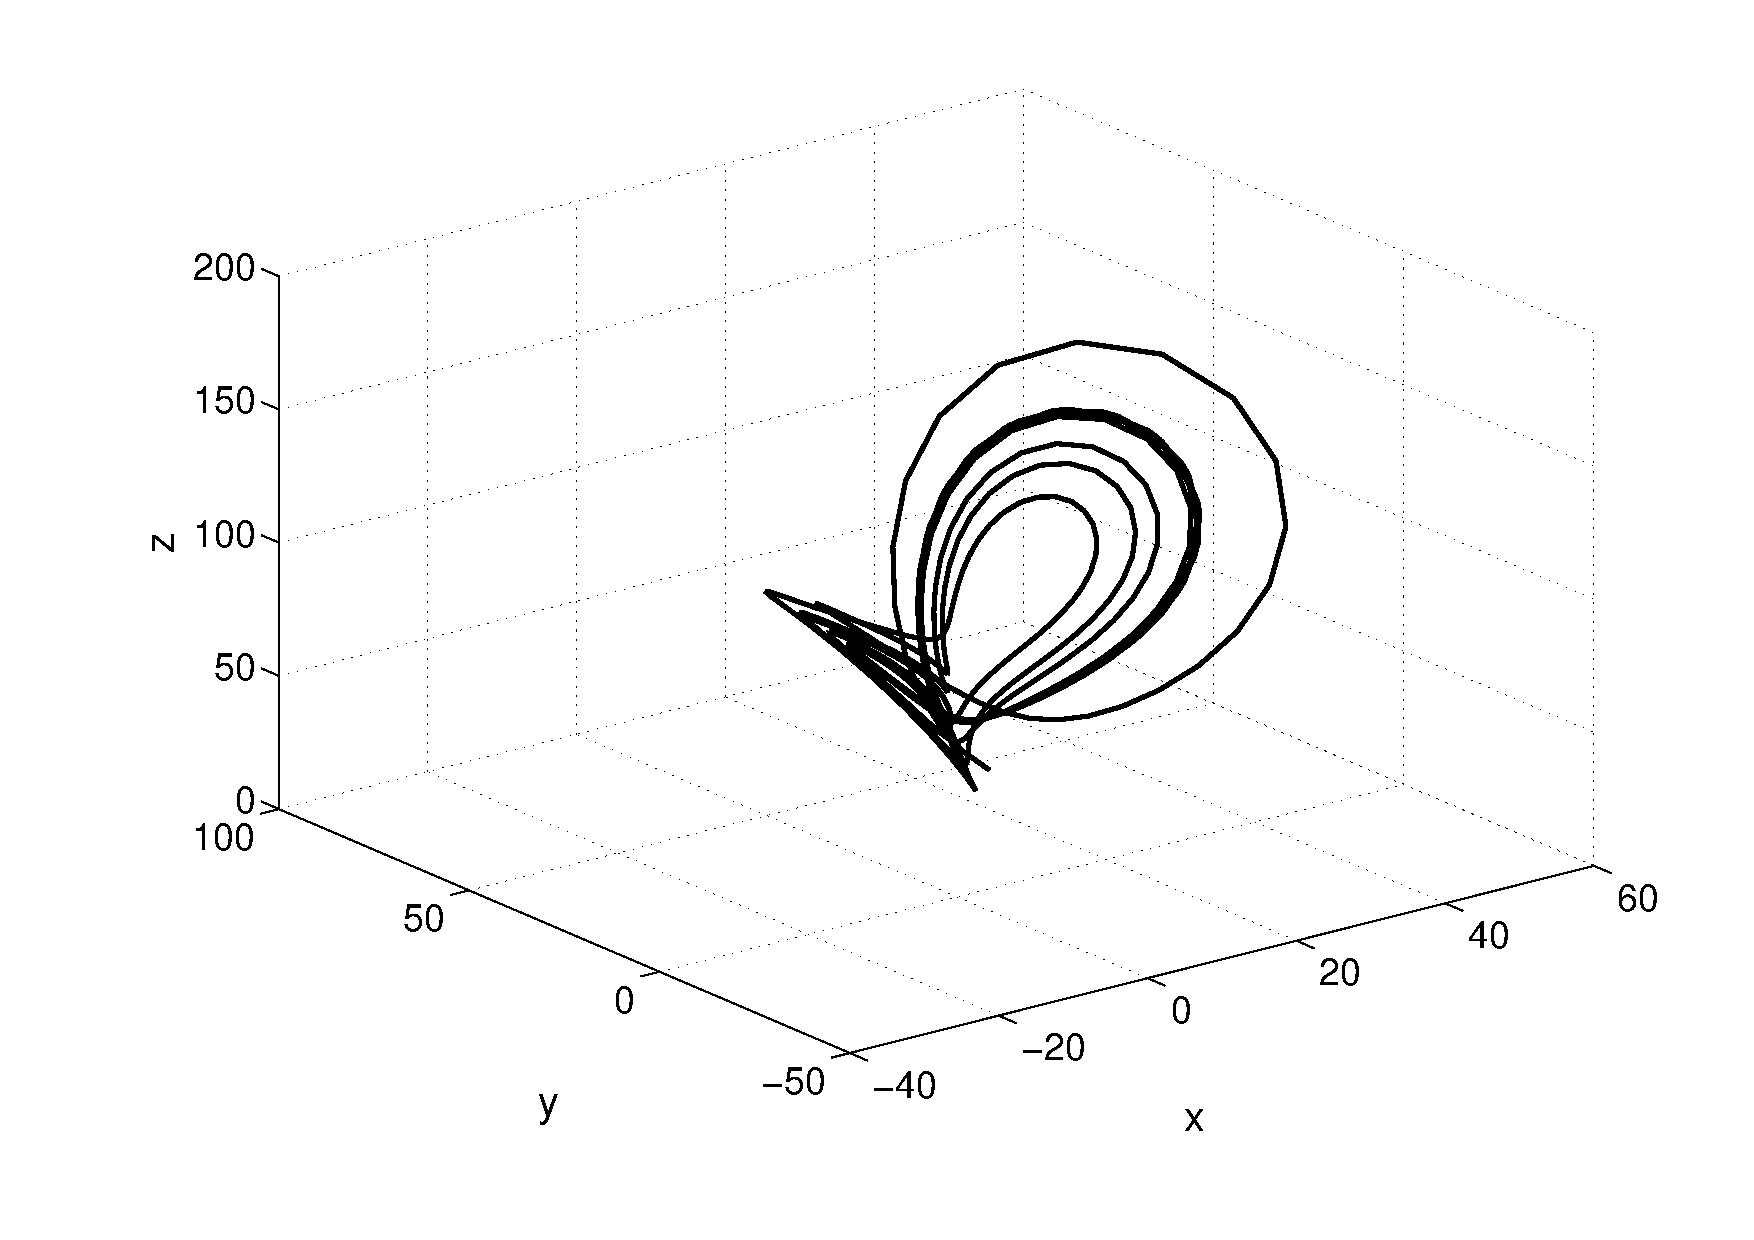
\includegraphics[scale=0.4, trim = 20mm 0mm 0mm 0mm, clip]
{./Figures/2-CauchyProblem/lorentz_3.pdf}
\caption{The Lorenz attractor.}
\end{figure}

The system routine for this problem should be written as follows: 

\begin{blueframed}
\begin{lstlisting}
subroutine  Lorenz_attractor(t, U,  F)        
    
     real, intent(in)  :: t
     real, intent(inout)  ::  U(:)
     real, intent(out) :: F(:)
      
     real :: x, y , z
	  
	 x = U(1); y = U(2); z = U(3)   

    	 F(1) =   a * ( y - x ) 
	 F(2) =   x * ( b - z ) - y 
	 F(3) =   x * y - c * z   

end subroutine 
\end{lstlisting}
\end{blueframed} 


As cuorisity, the following figures present the results of the system described
above. The results can be very different depending on the parameters ($a$, $b$,
$c$) of the system. 

\begin{multicols}{2}

\begin{figure}[H]
\centering
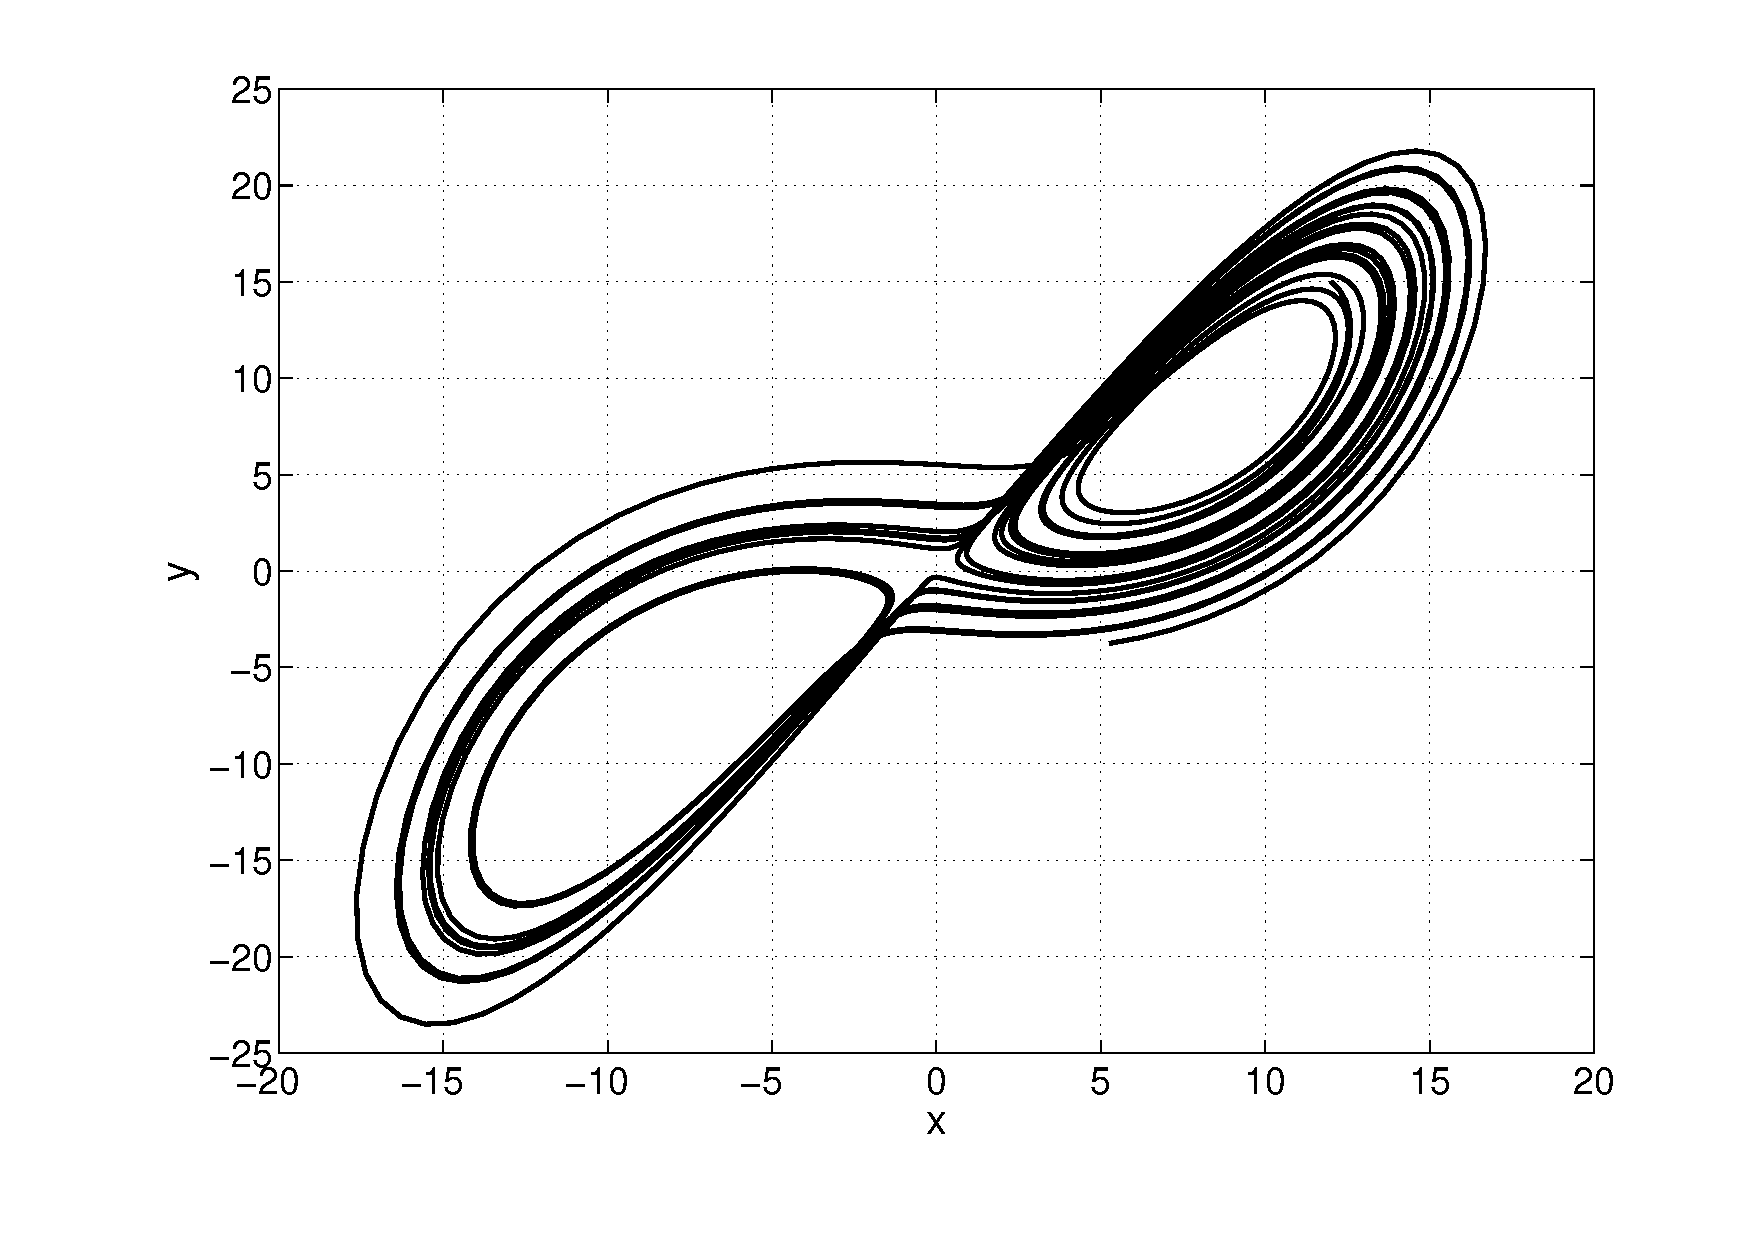
\includegraphics[scale=0.3, trim = 20mm 0mm 0mm 0mm, clip]
{./Figures/2-CauchyProblem/lorentz_xy.pdf}  \caption{2D plot ($x \:\: vs. \:
y$) of the Lorenz attractor with $a=10$, $b=28$ and $c=2.67$.} 
\end{figure}

\columnbreak

\begin{figure}[H]
\centering
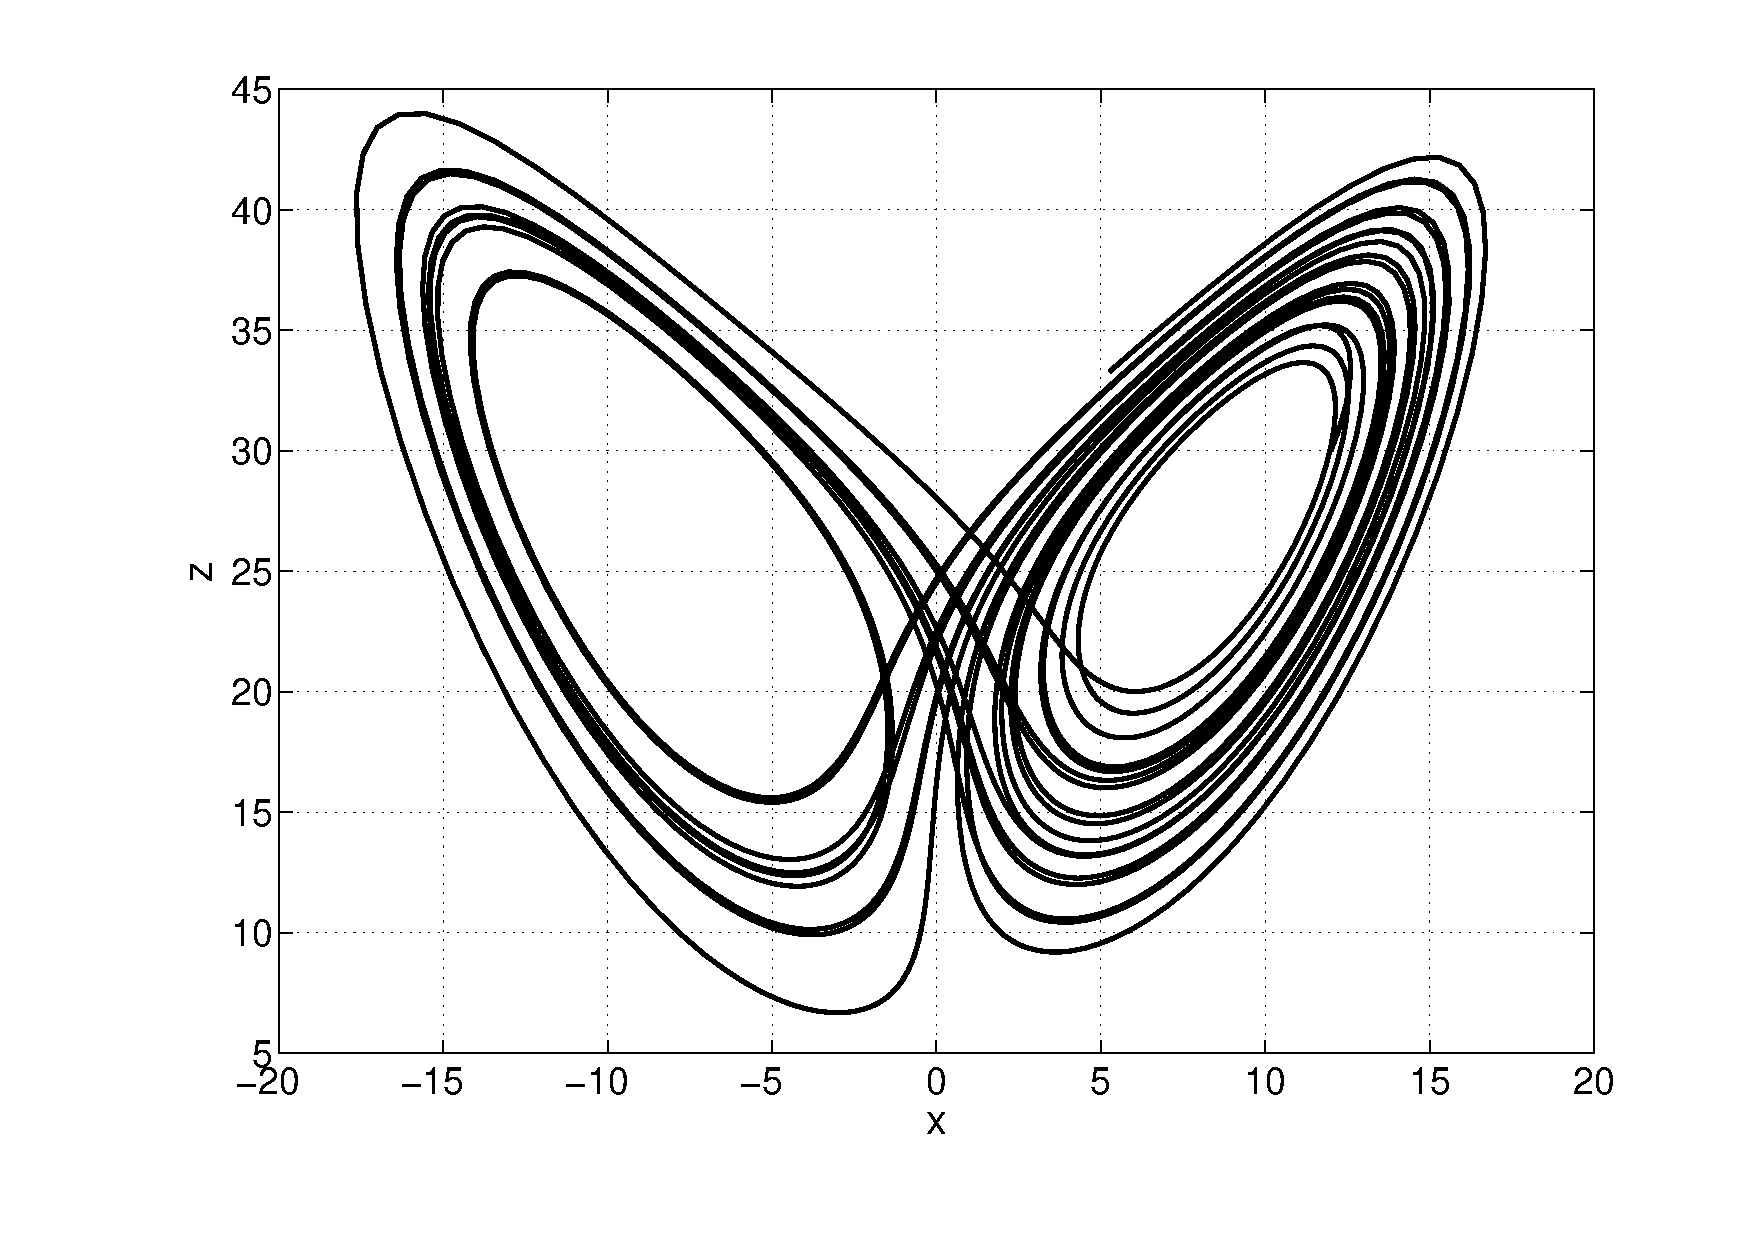
\includegraphics[scale=0.3, trim = 20mm 0mm 0mm 0mm, clip]
{./Figures/2-CauchyProblem/lorentz_xz.pdf}
\caption{2D plot ($x \:\: vs. \: z$) of the Lorenz attractor $a=10$,
$b=28$ and $c=2.67$.}
\end{figure}

\end{multicols}

\begin{multicols}{2}

\begin{figure}[H]
\centering
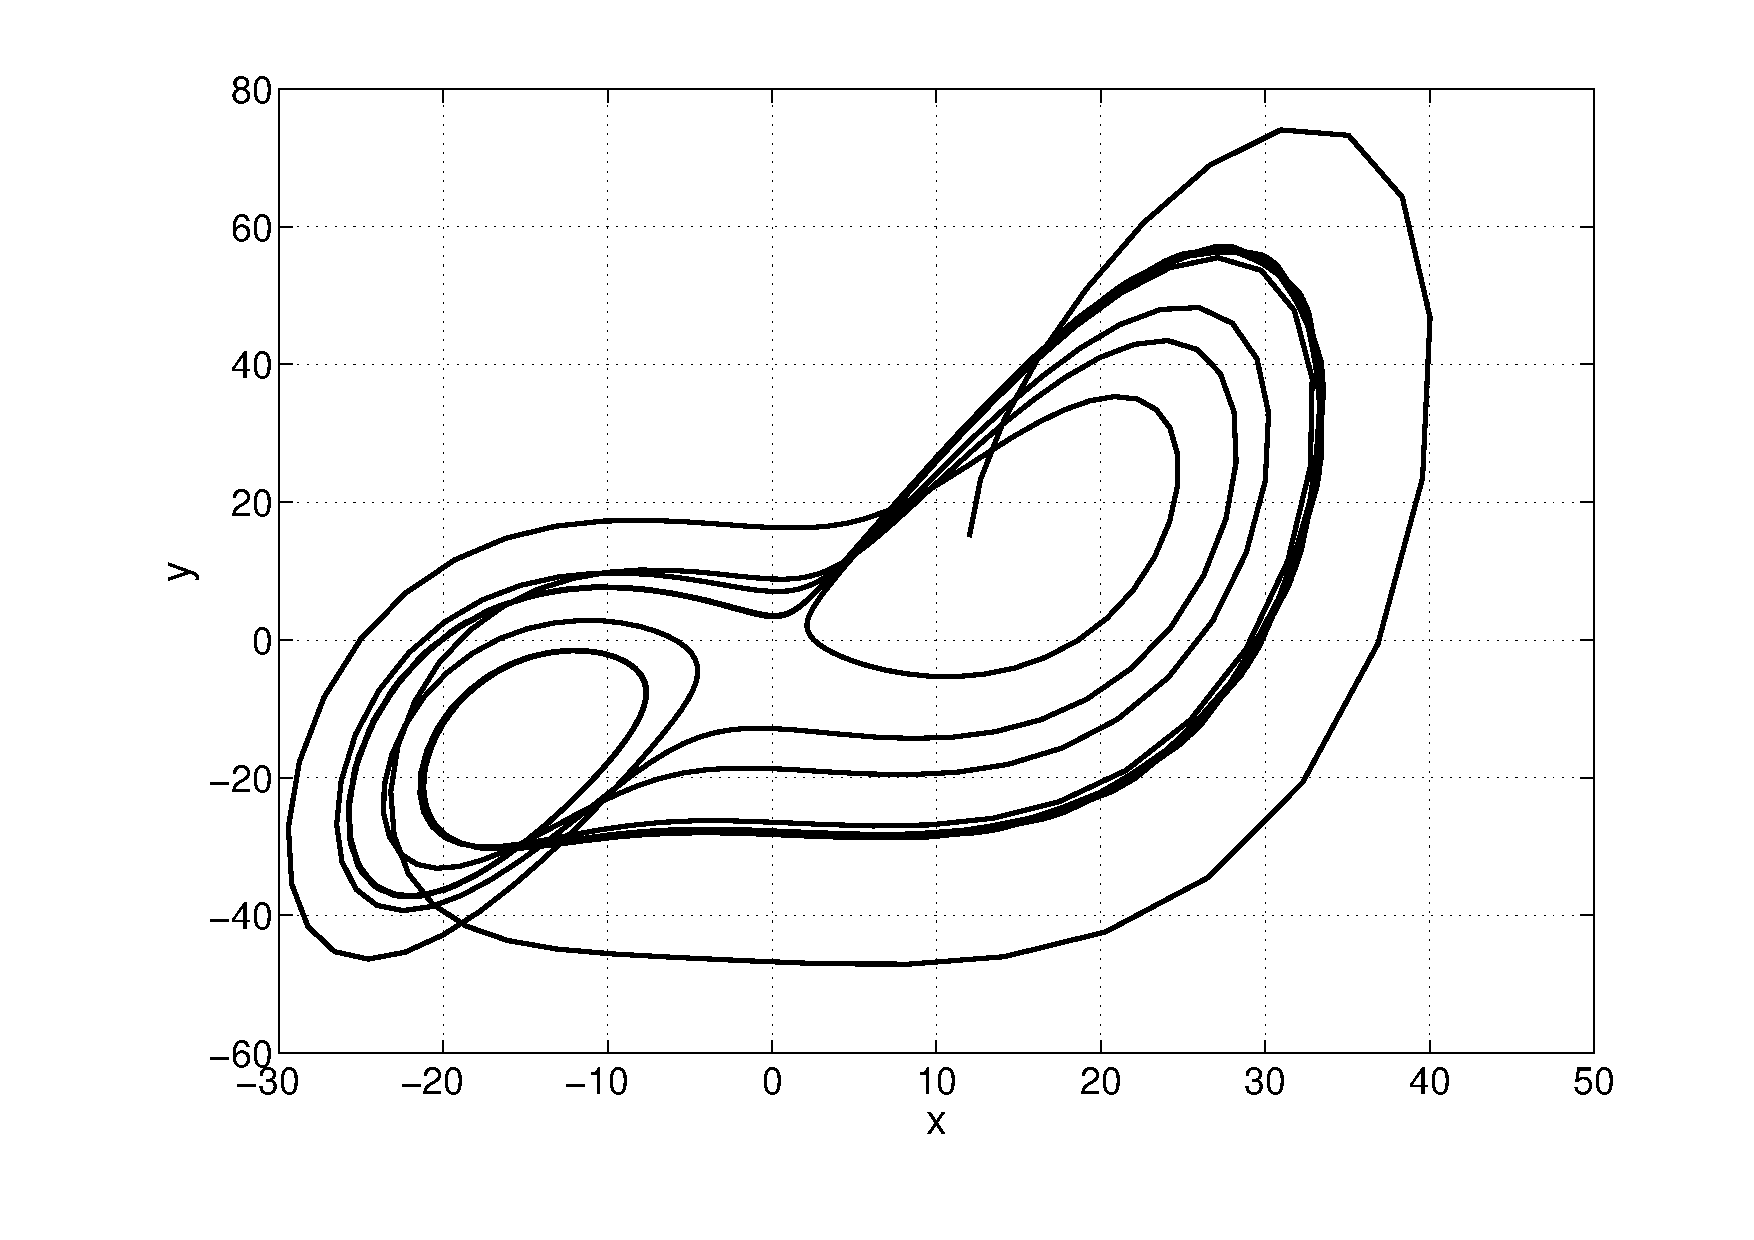
\includegraphics[scale=0.3, trim = 20mm 0mm 0mm 0mm, clip]
{./Figures/2-CauchyProblem/lorentz_xy2.pdf}
\caption{2D plot ($x \:\: vs. \: y$) of the Lorenz attractor with $a=10$,
$b=99.96$ and $c=2.67$.}
\end{figure}

\columnbreak

\begin{figure}[H]
\centering
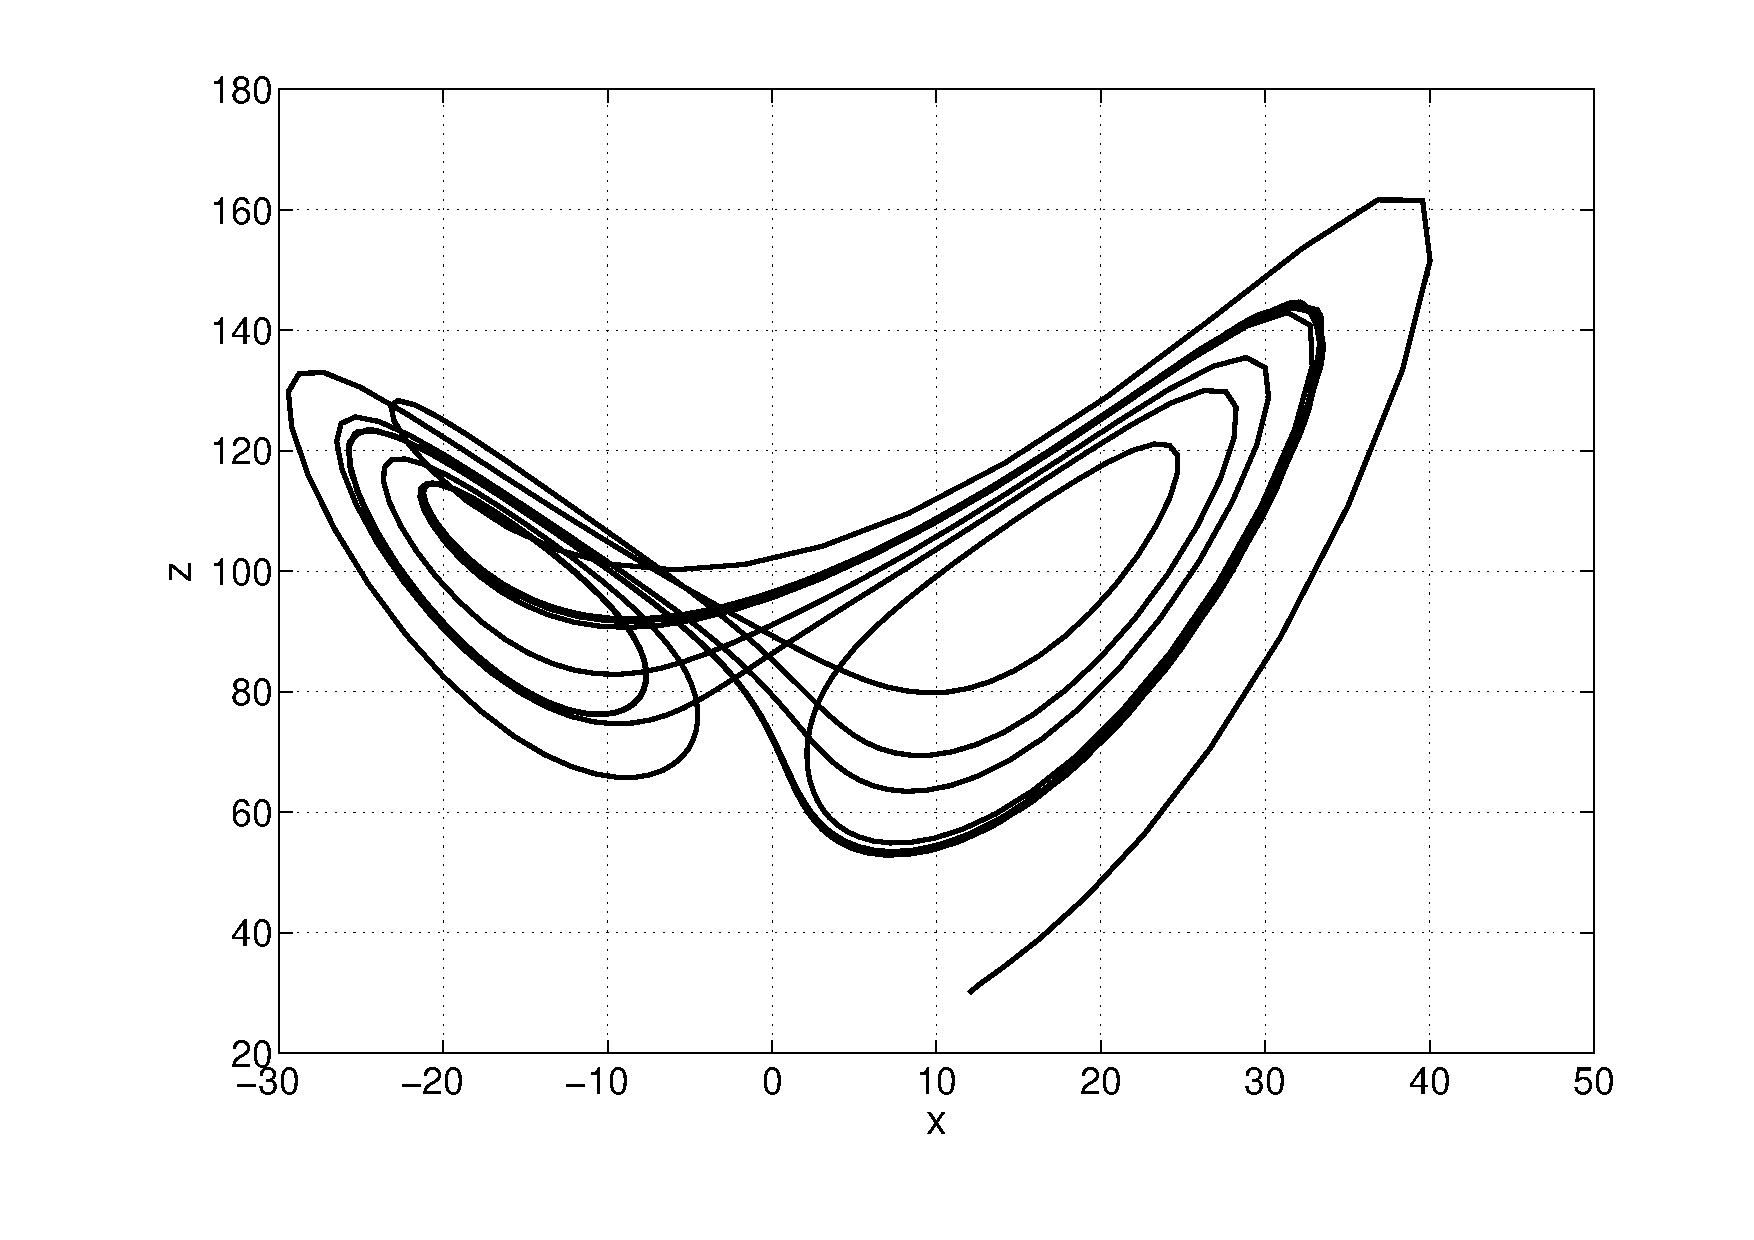
\includegraphics[scale=0.3, trim = 20mm 0mm 0mm 0mm, clip]
{./Figures/2-CauchyProblem/lorentz_xz2.pdf}
\caption{2D plot ($x \:\: vs. \: z$) of the Lorenz attractor $a=10$,
$b=99.96$ and $c=2.67$.}
\end{figure}

\end{multicols}

\newpage


\subsubsection*{EDP: Wave equation 2D}

\begin{blueframed}
{\begin{small}
\begin{lstlisting}
subroutine  Wave2D_equation(t, U,  F)            
              real, intent(in)  :: t
              real, intent(inout)  ::  U(:)
              real, intent(out) :: F(:)

  integer :: M 

  M = (Nx+1)*(Ny+1) 
 
  call Wave2D_equations(Nx, Ny, U(1:M), U(1+M:2*M), F(1:M), F(1+M:2*M)) 

contains 

	subroutine Wave2D_equations( Nx, Ny, P, W, Fp, Fw  ) 
	      integer, intent(in) :: Nx, Ny 
	      real, intent(inout) ::   P(0:Nx, 0:Ny),  W(0:Nx, 0:Ny) 
	      real, intent(out) :: Fp(0:Nx, 0:Ny), Fw(0:Nx, 0:Ny) 
	
	      real :: Pxx(0:Nx, 0:Ny), Pyy(0:Nx, 0:Ny) 
	
	 !** Boundary conditions 
	      call Newmann("x",0, P, 0.); call Newmann("x",Nx, P, 0.);
	      call Newmann("y",0, P, 0.); call Newmann("y",Ny, P, 0.); 
	
	  !** Wave equation
	      call Derivative( "x", 2, P, Pxx ) 
	      call Derivative( "y", 2, P, Pyy ) 
	
	      Fp =  W 
	      Fw =  4 * (Pxx + Pyy) 
	
	end subroutine 

end subroutine 

\end{lstlisting}
\end{small}}
\end{blueframed} 

\subsection{Temporal schemes}

The available temporal schemes are: 

\begin{itemize}
  \item Euler (\texttt{Euler})
  \item Leap frog (\texttt{Leap\_frog})
  \item Predictor-Corrector (\texttt{Predictor\_Corrector1})
  \item Adams-Bashforth (\texttt{Adams\_Bashforth} and
  \texttt{Adams\_Bashforth3})
  \item Crank-Nicolson (\texttt{Crank\_Nicolson})
  \item Runge-Kutta (\texttt{Runge\_Kutta4} and \texttt{Runge\_Kutta2})
  \item Inverse Euler (\texttt{Euler\_inverso})
\end{itemize}

The name between parenthesis is the name as it should be written in the
program in order to perform the procedure. If no procedure is specified, the
library will continue with \texttt{Runge\_Kutta4} by default. \\

For additional information about the different schemes, look into

 \textsc{\textbf{Juan A. Hern\'andez}, C\'alculo num\'erico en ecuaciones
 diferenciales ordinarias.}

\subsection{Outputs}

It is allowed to collect information from the resolution process using the
\texttt{Outputs} subroutine. \\

This procedure is called after every time step of the evolution problem, so a
great deal of data (both about the solution or the process) can be stored.\\

\begin {blueframed}
\begin{lstlisting}
subroutine Outputs(t,U,S)

             real, intent(in) :: t
             real, intent(inout) :: U(:)
             procedure (ODES_Outputs), optional :: S
             
             !...
             
end subroutine
\end{lstlisting}
\end{blueframed}

As we can see, the arguments to this routine are the time $t$ and the dependent
variable $U$. There is also an option to add a procedure, defined by the user,
to process the data. \\

As it has already been said, this routine is called after every time step of the
solving procedure, so the information can be taken (and plotted, if needed)
during the process or after the end of it. \\

Some useful commands for this routine are: 

\begin{itemize}
  \item \texttt{print*,} - It is useful in order to check the functionality of
  the process (sometimes the calculation is very long and, especially in the
  first stages of software development, we want to make sure that the program is
  working as expected, and waiting until the end of the process to check that
  something is not working might be a severe waste of time). \\
  \item DISLIN - this is a library which allows us to plot figures (quite
  rudimentary) directly from the code execution. It is useful in the same way as
  the \texttt{print} statement, but we are not going to use it for publishing
  results.

Some useful tools are \texttt{qplot( x, F, N )}, which represents N points of
the function $F=F(x)$ and \texttt{qplcon( F, Nx, Ny, NN);}, for plotting $NN$
isolines of a 2D function $F=F(x,y)$.\\

  \item \texttt{write(txt,fmt)} - this command allows the user to write the data
  in a \texttt{.txt} file that has to be defined. Also, one can choose
  the format (\texttt{fmt}) of the stored data. It is compulsory to open the
  file at the beginning:  \texttt{OPEN(UNIT=txt, FILE= 'results.txt',
  ACTION='write')} and close it (\texttt{close(txt)}), at the end. \\
  
\end{itemize}







\newpage

\subsection{Test}

The test routine is very simple: 

\begin {blueframed}
\begin{lstlisting}
subroutine test_mass_spring_damper

   call Cauchy_Problem_Solution( Domain = Time_Domain, & 
   				Initial_C =problem_IC,& 
   				System = mass_spring_damper, &
   				Scheme=Runge_Kutta4, &
    				Outputs=results)
end subroutine
\end{lstlisting}
\end{blueframed}

The \texttt{Cauchy\_Problem\_Solution} statement can be called as
well from the main program. However it is better to do it this way so the
program has its own checking tool and becomes independent from the main file. \\

If the purpose of the program is just to solve a given problem, the main file is
simple: 

\begin {blueframed}
\begin{lstlisting}
program main

    use example_mass_spring_damper

    implicit none


    call test_mass_spring_damper


end program
\end{lstlisting}
\end{blueframed}

However, for bigger structures where the resolution of the initial condition
problem is just a single step of the process, the main file might be a bit more
complicated. Anyway, the multilayered structure allows us to separate and to
work with this layer independently to the rest of the program construction.\\

\newpage

\subsection*{Results of the mass-spring-damper system}

The test case allows the validation of the routines.  The following figures
present the results obtained from two different simulations:  the conservative
system ($D=0$) and a damped system ($D=1$):

\begin{multicols}{2}

\begin{figure}[H]
\centering
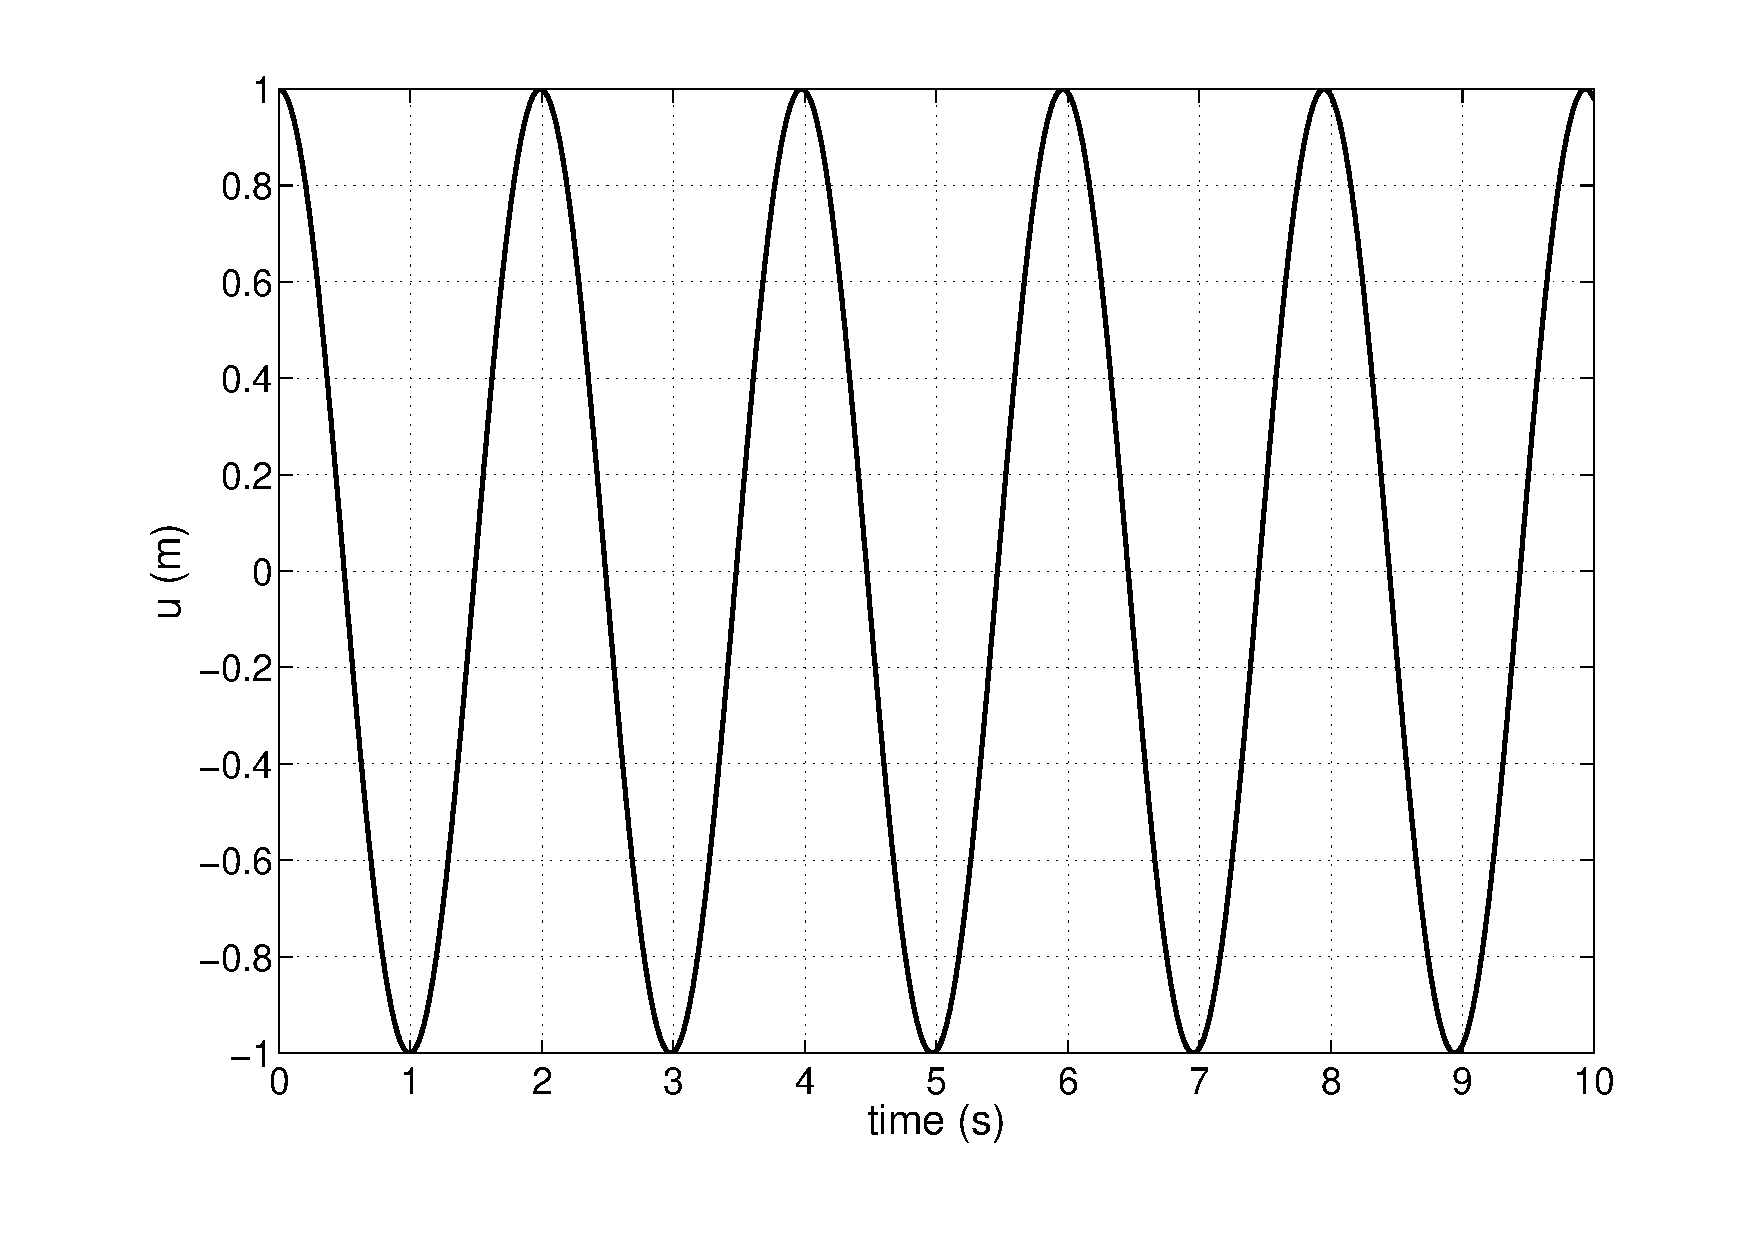
\includegraphics[scale=0.3, trim = 20mm 0mm 0mm 0mm, clip]
{./Figures/2-CauchyProblem/D=0.pdf}
\caption{Conservative system.}
\end{figure}

\columnbreak

\begin{figure}[H]
\centering
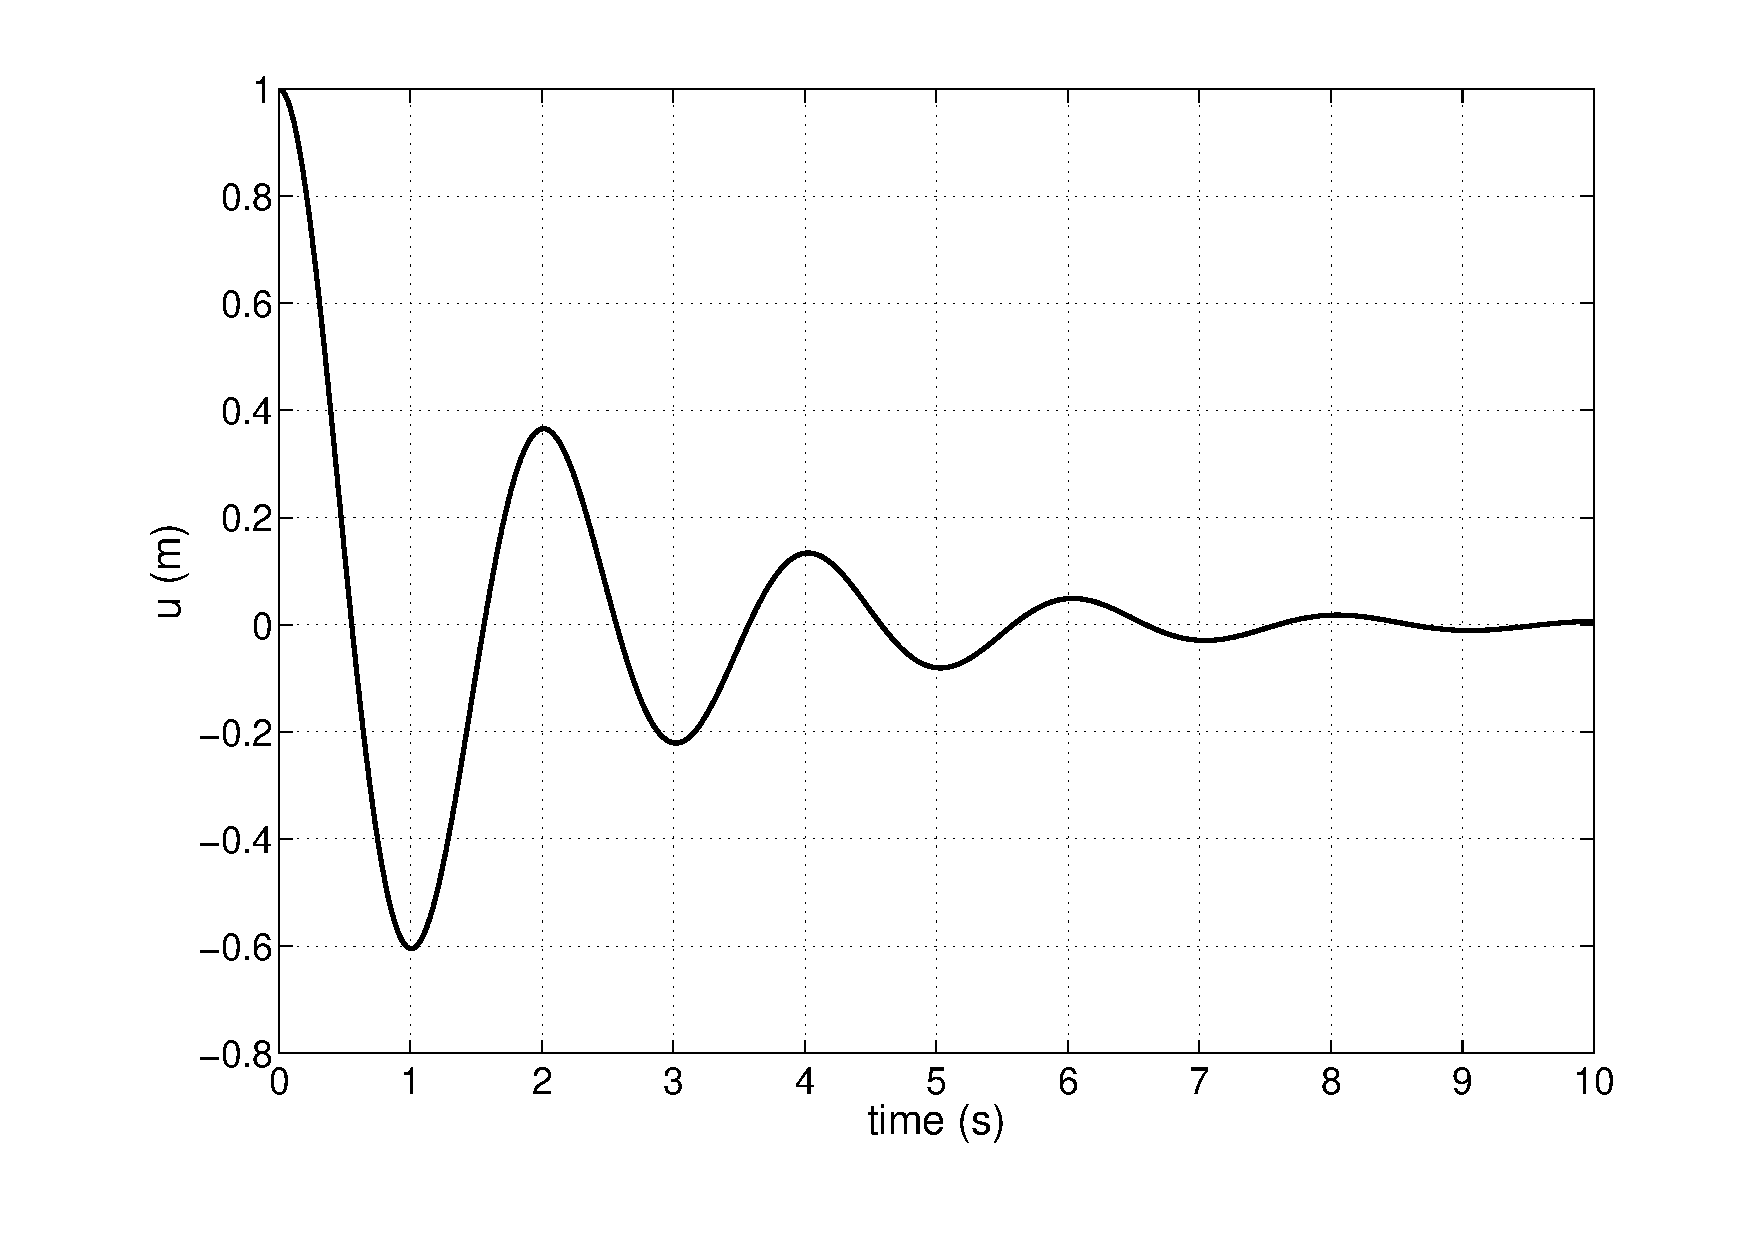
\includegraphics[scale=0.3, trim = 20mm 0mm 0mm 0mm, clip]
{./Figures/2-CauchyProblem/D=1.pdf}
\caption{Damped system.}
\end{figure}

\end{multicols}

\begin{multicols}{2}

\begin{figure}[H]
\centering
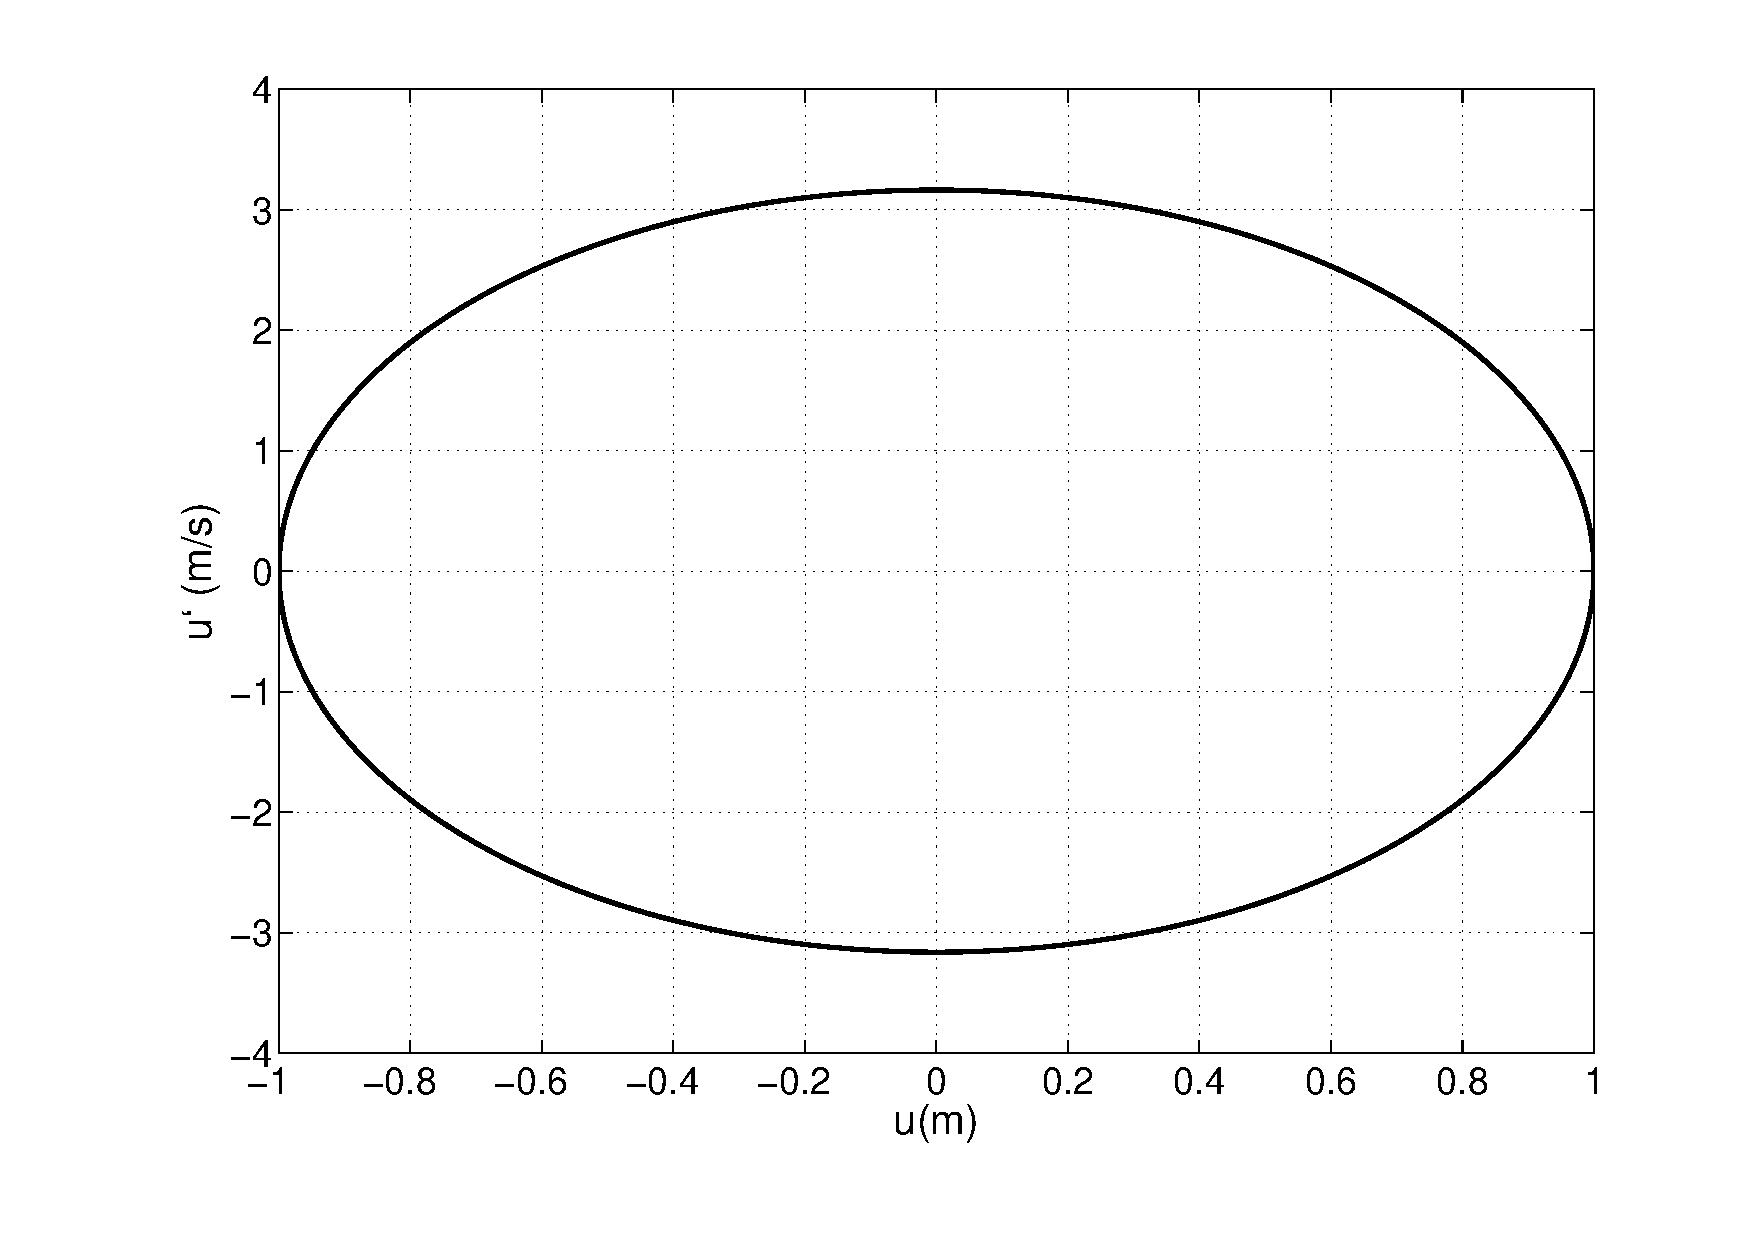
\includegraphics[scale=0.3, trim = 20mm 0mm 0mm 0mm, clip]{./Figures/2-CauchyProblem/D=0_uu.pdf}
\caption{Position ($u$) vs. velocity ($\dot{u}$) for the conservative system.}
\end{figure}

\columnbreak

\begin{figure}[H]
\centering
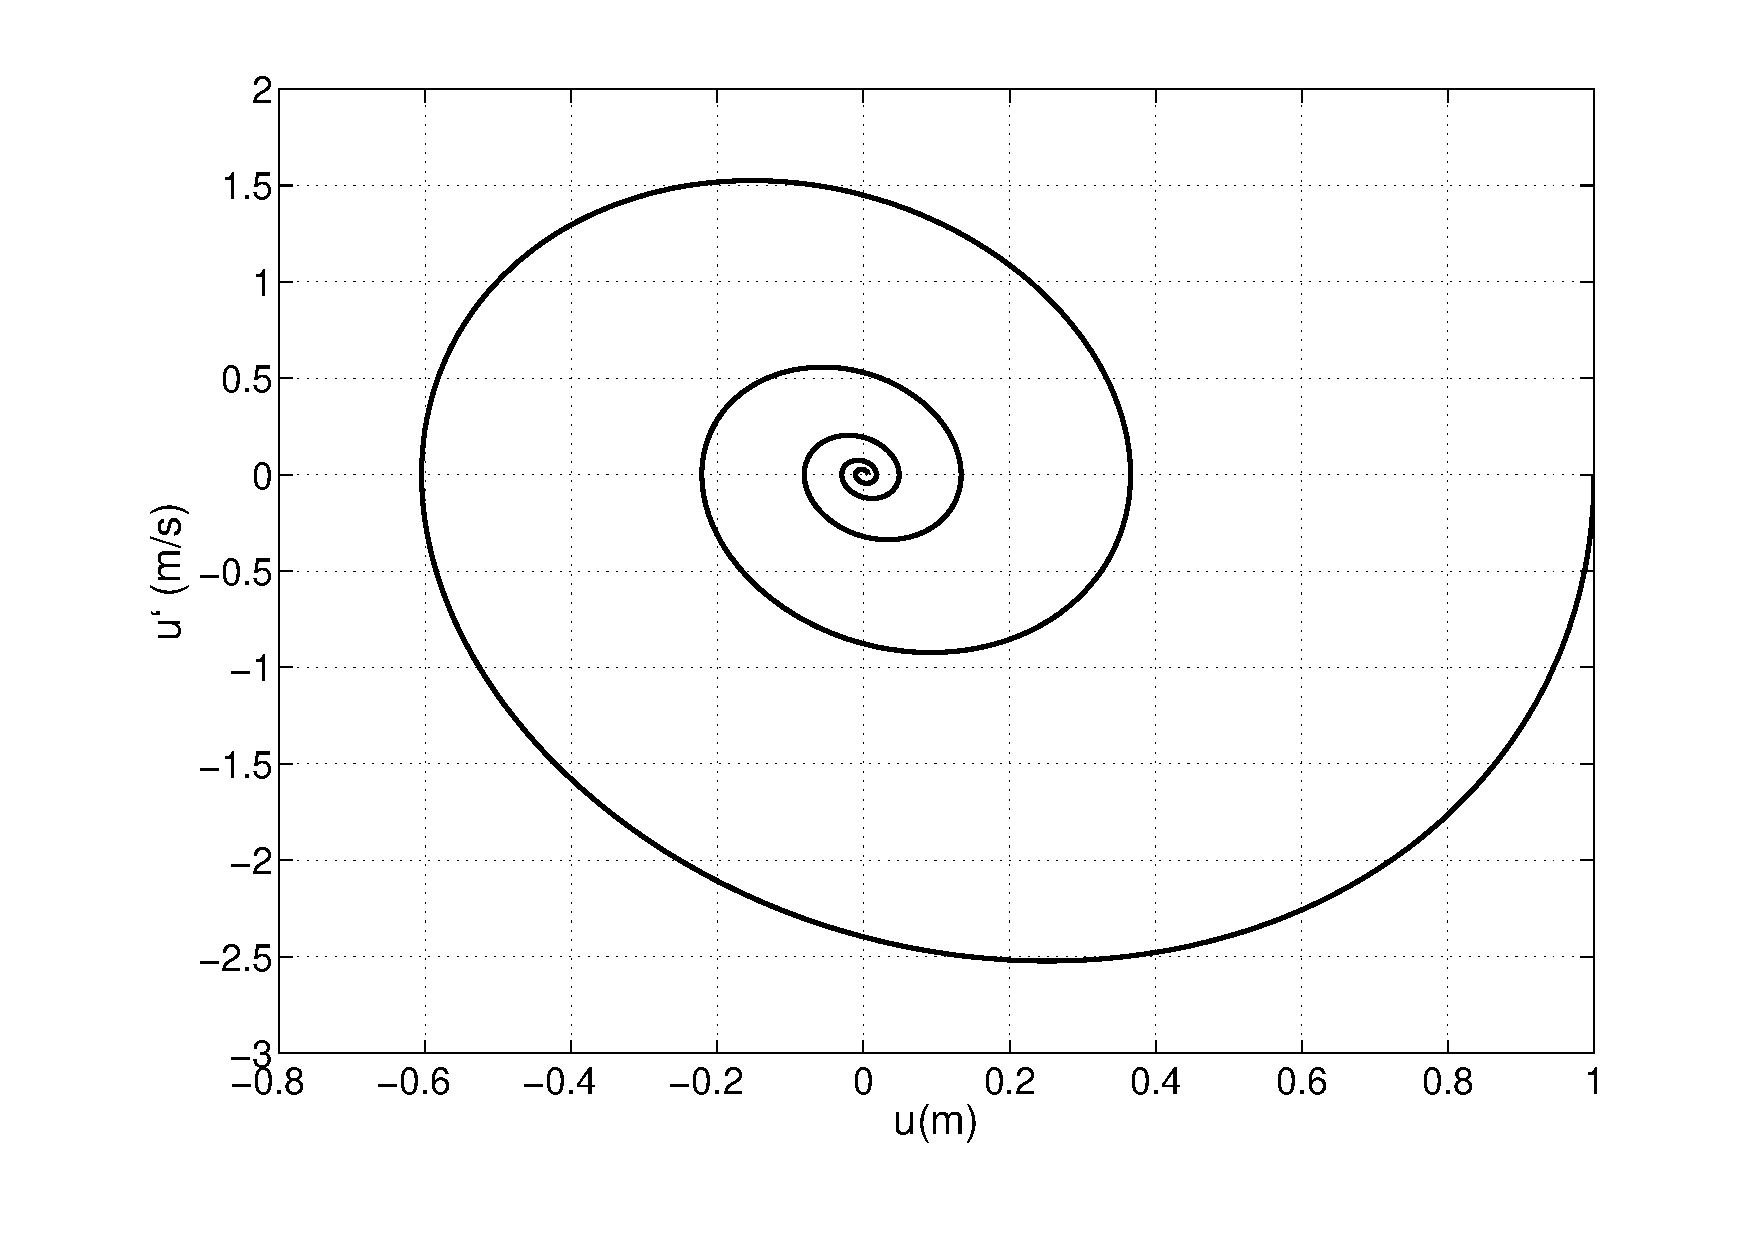
\includegraphics[scale=0.3, trim = 20mm 0mm 0mm 0mm, clip]{./Figures/2-CauchyProblem/D=1_uu.pdf}
\caption{Position ($u$) vs. velocity ($\dot{u}$) for the damped system.}
\end{figure}

\end{multicols}

This kind of easy examples are very useful for testing and validating the
software applications. Once again the results were successful, so the
functionality of the Cauchy module is assured. \\









\newpage
\chapter{Boundary Value Problem}

This paper holds the description of a software tool developed for
solving boundary value problems. This tool is prepared to be used as a black 
box where some inputs are given (equation, boundary conditions...) and the 
problem solution is obtained.
\\

With the aid of this manual, the reader should be able to build and solve a huge
variety of problems. \\

Specific syntax and procedures should be used in order to launch the solver
application for this problems. The rules and methods for these purposes
configures the Application Programming Interface (API) of this library. This
manual will help the reader with the commands and its functionality. 
\\

Please note that the theoretical explanation of Boundary Value Problems is
beyond the purposes of this brief manual. The idea is to give just the essential
information in order to \underline{use} this software tool. 
\\




%1.==========================BODY==============================================
\newpage

\section{Introduction}

A boundary value problem appears when a equation is to be solved inside a region
(space domain) according to some constraints which applies to the frontier of
this domain (boundary conditions). \\

First of all, we need to remember that, differently from the Cauchy's Problem,
where the initial condition ensures the uniqueness of the solution; a boundary
value problem has to be well written in order to find a unique solution. \\

Assuming that the problem is well posed, the software tool that we are
presenting here should be able to solve the equations. \\

This software is framed over the spatial discretization tool \footnote{Go to
\textbf{High Order Finite Difference API} to find further information.} and will
use specific procedures and methods from this library. The idea under the whole
project structure is to encapsulate the complexity so each problem would be easy
to solve using the appropriate level of this tree, calling the procedures
according to its API. \\

\begin{framed}


\begin{framed}
{\Large{\textbf {Application Layer}}}\\
\end{framed}

\begin{centering}

\begin{Large}
\hfill $\Downarrow \hspace{1cm} API_{BVP} \hspace{1cm} \Uparrow$ \hfill
\end{Large}
\end{centering}

\begin{framed}
{\large{\textbf {Boundary Value Problem ($BVP$)}}}\\

\begin{multicols}{2}

\begin{framed}
Linear Boundary Value Problem
\end{framed}

\columnbreak

\begin{framed}
Non Linear Boundary Value Problem
\end{framed}


\end{multicols}

\end{framed}

\begin{centering}

\begin{large}
\hfill $\Downarrow \hspace{1cm} API_{HOFD} \hspace{1cm} \Uparrow$ \hfill
\end{large}
\end{centering}

\begin{framed}
{\large{\textbf {High Order Finite Difference Library ($HOFD$)}}}\\

\begin{multicols}{2}

\begin{framed}
{\large{\textbf{Grids}}}\\

\hspace{0.5cm} Grid \hfill \framebox[3cm]{Grid initialization}\\

\end{framed}

\begin{centering}

\begin{large}
$\Updownarrow$
\end{large}

\end{centering}

\columnbreak

\begin{framed}
{\large{\textbf{Finite differences}}}\\

\hspace{0.5cm} Derivatives \hfill \framebox[3cm]{Derivatives}\\

\end{framed}

\begin{centering}

\begin{large}
$\Updownarrow$
\end{large}

\end{centering}

\end{multicols}


\begin{framed}

\begin{centering}

{{\textbf{Lagrange interpolation}}}

\end{centering}

\end{framed}



\end{framed}

\end{framed}


Any particular problem is to be written in the higher layer of this structure.
The call to the boundary value problem is to be declared
(respecting its API, $API_{BVP}$) in this level. The key of this philosophie is
that we just need to include this call in order to solve the problem. As we do
not need to calculate derivatives or grids when defining the problem, we
do not include these operators.\\

Then, when solving the problem, the \textit{box} $BVP$ will use the layers
underneath and return the solution of the problem. In the process we have not
written any routine for discretizing, meshing, differentiation\ldots  as the
operators are already configured in the lower layers, we just need to define
the problem and call the solver. \\

For the solver, there are two tools available: \textit{linear} and \textit{non
linear}. The linear problem is easier in terms of programming and computing, so
a specific procedure is developed. Please note that both the equation and the
boundary conditions \underline{must} be linear.\\

For more general purposes, the non linear solver has to be used.\\




\section{Linear Boundary Value Problems}

The linear boundary value problem is something in the shape of: 

\begin{Large}


$$\begin{cases}
\mathscr{L}(\mathbf{u})=0\\

+BCs
\end{cases}
$$\\

\end{Large}

where $\mathscr{L}$ is a linear operator. Thus, it can be transformed to the
usual linear problem appearance: 

$$[A]\cdot \{\mathbf{u}\}+\{\mathbf{b}\} =0 $$ 		

The solution then is simple if the matrix $[A]$ is not singular. 

$$\{\mathbf{u}\}=-[A]^{-1}\{\mathbf{b}\} $$ 	\\

This procedure is encapsulated in the solver subroutine, and the only thing that
is needed is the proper definition of the problem, according to the following
structure:\\


\begin{blueframed}
\begin{lstlisting}
call Linear_Boundary_Value_Problem(  x_nodes = x, Order = N, &
                     Differential_operator = Equation, &
                     Boundary_conditions = BCs, Solution = U )

\end{lstlisting}
\end{blueframed}

The arguments of this assignment must be written regarding the problem's API. In
the following pages we are going to focus on the explanation of these items.
Some remarks would be added concerning the solver operation, however, a deep
explanation of the procedure is not the point of this manual. \\

\newpage


\subsection{Application programming interface}

Two routines have been implemented for solving 1D and 2D linear boundary value
problems. Both problem must be called equally with the sentence \texttt{call
Linear\_Boundary\_Value\_Problem(\ldots)} and the solver will choose the
appropriate procedure (1D or 2D), depending on the input arguments. \\

For the shake of simplicity, let's begin with the explanation of procedure for
1D problems.
The extension for 2D problems will be pretty much the same, taking into account some
particularities. However, \textit{from the user point of view}, the only
remarkable difference would be found in the inputs arguments when writing the
\texttt{call} statement. \\

The solver for 1D problems will need the spatial region where the program is to
be solved, the problem definition and the boundary conditions. Additionally, the
order of interpolation is needed (use high order interpolation for a better
approximation of derivatives). \\

Basically, the solver does the transformation of the problem to the
linear operator seen in the previous page. This structure holds both the
equation and the boundary conditions, that are assumed to be linear too
(otherwise, check the following section for non linear problems). \\

Once the problem is transformed, the solver executes a LU factorization in order
to find the solution. If the problem is well defined, the matrix $[A]$ will not
be singular, so an unique solution exists.\\

Finally, the solver returns the solution.\\

Regarding the software, all this procedure is held inside the following
subroutine: \\

\begin{blueframed}
\begin{lstlisting}
subroutine Linear_Boundary_Value_Problem1D( x_nodes, Order, &
 				Differential_operator, &
 				Boundary_conditions, Solution)
        
     real, intent(inout) :: x_nodes(:)
     integer, intent(in) :: Order
     procedure (DifferentialOperator) :: Differential_operator
     procedure (BC) ::  Boundary_conditions
     real, intent(out) :: Solution(:) 

\end{lstlisting}

\end{blueframed}


All the input arguments must be defined as none of them is declared with the
\textit{optional} label. The syntax is very clear and logical, however some remarks need to
be clarified, so let's look at them in the following pages. \\

\newpage

\subsubsection{Space Domain}

The space domain is to be defined as a vector variable ($x(:)$). As it is an
\texttt{inout} argument, it must be allocated \textit{before} calling the
solver. \\

Once imported to the solver, first of all the subroutine will check if the
vector has already a value. By default the program will assign a space domain
$x \in [-1,1]$; but it can be changed if needed just giving a value to the
$x_{nodes}$ vector before calling the solver. This way, when the routine checks
the vector, if it has already been given a value it performs the mesh and then
transforms the domain according to the upper and lower bound of the initial
vector. \\

By default, the mesh will be \texttt{nonuniform} but it can be changed if
needed. \\

Please be careful with the space domain definition, because the program will not
work if the upper and lower bound of $x_{nodes}$ do not match the points
where the boundary conditions are applied. \\

For 2D problems two separate arguments will be included instead of one:
$x_{nodes}$ and $y_{nodes}$, matching the following structure: \\

\begin{blueframed}
\begin{lstlisting}
subroutine Linear_Boundary_Value_Problem2D( x_nodes, y_nodes, &
 				Order, Differential_operator, &
 				Boundary_conditions, Solution)

\end{lstlisting}
\end{blueframed}

However the sentence to call the solver from the user's application layer is the
same as we have already seen in the previous pages: \\

\begin{blueframed}
\begin{lstlisting}                    
call Linear_Boundary_Value_Problem(  x_nodes = x, y_nodes = y, & 
                  Order = N, Differential_operator = Equation, &
                  Boundary_conditions = BCs, Solution = U )

\end{lstlisting}
\end{blueframed}

\subsubsection{Interpolation order}

The interpolation order is an input argument which has to be an integer for
obvious reasons. Also, it must be greater than two and lower than the number of
points of the discretization:

$$
N \text{points, then } \mathbf{x\_nodes}(0:N) \text{, thus, \textbf{order}} \le
N-1 $$\\

This order will be used to compute the interpolating polynomials and the
derivatives, using the module \texttt{finite\_differences}. \\

\newpage

\subsubsection{Differential operator}

The differential operator will be the equation of the problem that is to be
solved. This must be declared as a function: 

\begin{blueframed}
\begin{multicols}{2}
\hfill $\mathscr{L}(u)=0  \Longrightarrow$

\columnbreak
\begin{lstlisting} 
function Equation(x,u,ux,uxx)
\end{lstlisting}

\end{multicols}
\end{blueframed}

Let's bring some light to this point with an easy example. Imagine the following
problem:

$$ \frac{\delta u}{\delta x}+ x\cdot u = sin(x)
$$


$$ \text{So: }\mathscr{L}(u)= \frac{\delta u}{\delta x}+ x\cdot u - sin(x)
=0$$\\

The function should be written as follows: 

\begin{blueframed}
\begin{lstlisting} 
real function Equation(x,u,ux,uxx)
		real, intent(in) :: x, u, ux, uxx 
    
		Equation = ux + x*u - sin(x)
		
end function

\end{lstlisting}
\end{blueframed}

Very easy: as it can be seen it is written \underline{just the same} as in the
papers and there is no need to worry about derivatives or discretization as the
solver will give the values when calling the equation (they are input arguments to this
function). This is the most powerful characteristic of our software.\\

For 2D problems, the input arguments to the function will be also the $y$
derivatives: 
\begin{blueframed}
\begin{lstlisting} 
real function Equation(x, y, u, ux, uy, uxx, uyy, uxy) 

\end{lstlisting}
\end{blueframed}

Please, remark the order in which the arguments are specified because the solver
will call the procedure with this structure. Also, even if the $uxy$  derivative (for
example) is not needed for your problem, include it anyway because the
solver will call the equation although some arguments might be useless.\\

 An other option is to change the root file \texttt{Boundary\_value\_problems }
 in order to customize it to particular problems.
However I will not recommend that unless the user is completely sure of what to
do. \\

\newpage

\subsubsection{Boundary conditions}

The philosophy for the boundary conditions is the same. There is no need to
specify \textit{Dirichlet} or \textit{Neumann} conditions, just write the
statement as usual. For example: 

$$ BCS: \begin{cases} u(x=a)=0;\\ \frac{\delta u}{\delta x}|_{x=b}=0 \end{cases}
$$\\

These boundary conditions should be written as follows: 

\begin{blueframed}
\begin{lstlisting}
real function BCs(x, u, ux) 
	real, intent(in) :: x, u, ux 
           
	if (x==a) then
                      BCs = u 
	elseif (x==b) then
                      BCs = ux 
	endif
end function  
\end{lstlisting}
\end{blueframed}

Once again, it is important to respect the arguments of the function for the
same reasons as the ones listed previously.\\

\subsubsection{Solution}

The solution of the problem is a vector containing the function value in the
points of the discretization: $U=U(0:N)$. \\

For 2D problems, the solution is an array which dimension is: $U=U(0:N_x,
0:N_y)$. \\

\subsection{Test Linear Boundary Value Problem}

After the definition of this arguments, the solver is launched as follows. \\

\begin{blueframed}
\begin{lstlisting}
call Linear_Boundary_Value_Problem(  x_nodes = x, Order = N, &
                     Differential_operator = Equation, &
                     Boundary_conditions = BCs, Solution = U )

\end{lstlisting}
\end{blueframed}

In the following page an example is presented.\\


\newpage
\subsection*{Example: rod of variable cross section}

\begin{blueframed}
\begin{lstlisting}
module example_rod

	use Boundary_value_problems

	implicit none

	contains

	subroutine test_rod

  		 use dislin


   		 implicit none

		integer, parameter :: N=10
		real :: x(0:N), U(0:N)
	
		real :: x0=0d0 , xf=1d0
		integer :: i

       	 	x = [ (x0 + (xf-x0)*i/N, i=0, N) ]

  		 call Linear_Boundary_Value_Problem( x, &
  		 			4, Equation, BCs, U )

	!plots
       	call scrmod('revers')
       	call qplot(x, U, N+1)

    	contains


            subroutine area(x, A, dA)

                real, intent(in) :: x
               real, intent(out) :: A, dA

              real, parameter :: A0=1.
              real :: L
              	L=xf-x0

                A=A0*exp(-x/(1d0*L))

               dA= -A0/(1d0*L)*exp(-x/(1d0*L))

            end subroutine

   	 	real function Equation(x, u, ux, uxx)

           real, intent(in) :: x, u, ux, uxx

           real :: A, dA

           call area(x, A, dA)

           Equation = uxx + ux*dA/(1d0*A)

    end function

    real function BCs(x, y, yx)

           real, intent(in) :: x, y, yx

           real, parameter :: E = 1. , P=1.
           real :: A, dA


         if (x==x0) then
                      BCs = y

         elseif (x==xf) then

                     call area(x, A, dA)
                      BCs = yx - P/(1d0*E*A)
         else
             write(*,*) "Error_BCs_x=", x
             write(*,*) "a,b=", x0, xf
             read(*,*)
         endif

    end function

end subroutine

end module example_rod


program main

  use example_rod

  implicit none

	call test_rod

end

\end{lstlisting}

\end{blueframed}

\newpage

\section{Non Linear Boundary Value Problems}

The tool for non linear problems follows the same philosophy as the one
presented before. The idea is to be as simple as possible. \\

There are only two remarkable differences: 

\begin{itemize}
  \item The variable \texttt{Solution} was an output argument to the linear
  subroutine. This time it is an \texttt{inout} argument. 
  \item A non linear solver is needed.
\end{itemize}

The subroutine structure is presented under these lines. A 2D extension is also
available. We will talk about it a bit later. 

\begin{blueframed}
\begin{lstlisting}
subroutine Non_Linear_Boundary_Value_Problem1D( x_nodes, Order,&
					Differential_operator, &
					Boundary_conditions, &
					Solver, Solution)

     real, intent(inout) :: x_nodes(0:)
     integer, intent(in) :: Order
     procedure (DifferentialOperator) :: Differential_operator
     procedure (BC) ::  Boundary_conditions
     procedure (NonLinearSolver), optional:: Solver
     real, intent(inout) :: Solution(0:)

\end{lstlisting}

\end{blueframed}

\subsection{ Non linear solver and solution}

A non linear solver is needed in order to perform the iteration. It is declared
as an optional argument, so if no method is declared, the program will use one
by default. \\

Basically, the operations that the subroutine
\texttt{Non\_Linear\_Boundary\_Value\_Problem} performs can be summarized as
follows: 

\begin{itemize}
  \item Meshing. With the idea explained before: if a region is declared the
  mesh bounds will match those points; otherwise the program will assume
  $[-1,1]$.
  \item Boundary conditions discretization. 
  \item Discretization of the system equations.
\end{itemize}

After these operations, an extrapolation of the problem can be done \footnote {In the linear case,
the problem is reduced to $A\cdot U + B=0 $, and the solution is immediate.}: the
problem is reduced to something in the shape of $F(U)=0$. This is to say
that for any given $U$ a value of $F(U)$ is obtained; where the operator $F$
holds the system equations and the boundary conditions. \\

Then, the nonlinear solver is applied to this function, attemping to find the
$U$ that makes $F(U)=0$. For this purpose, an initial point should be given and
that is whay the argument \texttt{Solution} is declared as \texttt{inout}. If
\texttt{Solution} has been given a value, then this value will be taken as
initial point; otherwise, the initial point will be $U_j = 0$.  \\

First of all let's look to how the function $F$ is obtained: 

 \begin{blueframed}
 \begin{lstlisting}
 
 ! subroutine non_linear_boundary_value_problems
    contains

        subroutine System_BVP(U, F)
                real, intent (in) :: U(:)
                real, intent (out) :: F(:)

                call Difference_equation(x_nodes, U, F)

        end subroutine


        subroutine Difference_equation(x, W, F)
                real, intent(in) :: x(0:), W(0:)
                real, intent(out) :: F(0:)

                real :: Wx(0:N), Wxx(0:N)

                integer :: k

                call Derivative( "x", 1, W, Wx)
                call Derivative( "x", 2, W, Wxx)

               !  ***  boundary conditions
                F(0) = Boundary_conditions( x(0), W(0), Wx(0) )
                F(N) = Boundary_conditions( x(N), W(N), Wx(N) )

               !  *** inner grid points
          do k=1, N-1
            F(k) = Differential_operator( x(k), W(k), Wx(k),&
            					 Wxx(k) )
          enddo
               
         end subroutine


end subroutine
 
 \end{lstlisting}
 
 
 \end{blueframed}

There are two levels: in the first level we just declare the $F=F(U)$, while in
the second level the assignments of equations and boundary conditions are done.
\\


$$ \mathbf{U} \Longrightarrow \boxed{System\_BVP} \Longrightarrow \mathbf{F}$$
$$ \hfill \Updownarrow $$
$$ \boxed{difference\_equations}$$\\

Proceeding this way, a single variable function is obtained. Thus, any procedure
for solving nonlinear functions (Bisection, Secant, Newton-Raphson \ldots ) can be
used to find the solution.\\

The interface to this procedure is: 

\begin{blueframed}
\begin{lstlisting}
       subroutine  NonLinearSolver(Function, x)
       use system_interfaces
          procedure(System_BVP) :: Function
         real, intent(inout) :: x(:)
       end subroutine  NonLinearSolver
\end{lstlisting}
\end{blueframed}

So any method can be applied if it matches this structure. \\

As the solver is declared as an \texttt{optional} argument to the subroutine, if
no method is specified, the program will continue with the one by default (a
Broyden method is already implemented). However, there is the possibility of
adding any other procedure just declaring it when lauching the problem
initialization. 

\begin{blueframed}
\begin{lstlisting}
call Non_Linear_Boundary_Value_Problem( x_nodes = x, Order=4, &
                             Differential_operator= Equation, &
                             Boundary_conditions= BCs, &
                             !(Solver = user_defined, &)
                             Solution = U)
\end{lstlisting}
\end{blueframed}

Usually, the convergence of non linear methods depends on the initial point of
iteration. It can be changed giving a different value for $U$ before the
\texttt{call} statement. \\

The discussion about convergence, algorithms and methods for finding the roots
of nonlinear expression is beyond the purposes of this paper. Here, only a brief
explanation of the software is presented in order to use it and also in order to
know the possibilities and options that this tool provides. \\

\subsection{ 2D non linear problems}

2D problems will be treated the same way as 1D. In fact, the most part of the
code is interchangeable. \\

As we have said, the boundary value problem, the equations and its boundary
conditions, is reduced to an expression $F=F(U)$. Then, following the same
philosophy, the procedure is going to be the same, just taking into acount that
the number of variables is increased. \\

As we have said when dealing with linear problems, the solution will be an array
holding the value of the target function in the points of the discretization.
Then: 

$$
U(x,y) \Longrightarrow U_{ij}; \:\:\: i \in (0,N_x) \:\:\: j \in (0,N_y)
$$\\

The idea is to hold all the unknown variables in a vector, so the same methods
as the ones explained before could be used. This operation is encapsulated
inside the subroutine. \\

\begin{multicols}{2}


From $U=U(:)$ to $UU=UU(:,:)$:\\

\begin{blueframed}
\begin{lstlisting}
UU = reshape(U, [Nx+1, Ny+1])
\end{lstlisting}
\end{blueframed}

\columnbreak

From $FF=FF(:,:)$ to $F=F(:)$:

\begin{blueframed}
\begin{lstlisting}
F=reshape(FF, [ M ]);
\end{lstlisting}
\end{blueframed}

\end{multicols}

So, the algorithm can be summarized as follows: 


$$ \mathbf{U} \Longrightarrow \boxed{\hspace{2cm}System\_BVP\hspace{2cm}}
\Longrightarrow \mathbf{F}$$ 
$$ \hfill UU=reshape(U)\Downarrow  \hspace{2cm} \Uparrow F=reshape(FF) \hfill$$
$$ \boxed{difference\_equations}$$\\

And, as we have said, the nonlinear solver will just \textit{see} the function
\texttt{System\_BVP}, so the routines are the same as the ones for 1D problems.
\\


However, from the user's point of view, this procedure is hidden. The only
important thing will be the argument declaration in the function call: 

\begin{blueframed}
\begin{lstlisting}
call Non_Linear_Boundary_Value_Problem(x_nodes = x, y_nodes =y,&
		         Order = 5, &
                         Differential_operator = Equation,  &
                         Boundary_conditions = BCs,&
                         !Solver=user_defined,&
                         Solution = U )
\end{lstlisting}
\end{blueframed}

Where $x$ and $y$ should be vectors and $Solution$ is an array
of dimension $(0:N_x,0:N_y)$. The functions \texttt{Equation} and
\texttt{BCs} should be written the same way as they have been written when
dealing with linear problems.\\

In the following pages an example is presented in order to highlight the most
important ideas. \\


\newpage

\subsubsection* {Example of application}

The following problem is proposed: \\

$$ u\cdot \left(\frac{\delta^2 u}{\delta x^2}+\frac{\delta^2 u}{\delta
y^2}\right)=0$$

With the boundary conditions: 

$$ u(x=0,y)=0; \;\; u(x=1,y)=y $$
$$ u(x,y=0)=0; \;\; u(x,y=1)=x $$

The problem is useful as proof of concept because an analytic solution can be
obtained:

$$u(x,y)=x\cdot y$$

The following figures present the results obtained using two different meshes
with $10$ and $15$ points (left and right figures). In both cases one can see
the accuracy of the solution, which is enough to prove that this module is working as expected. 

\begin{multicols}{2}

\begin{figure}[H]
\centering
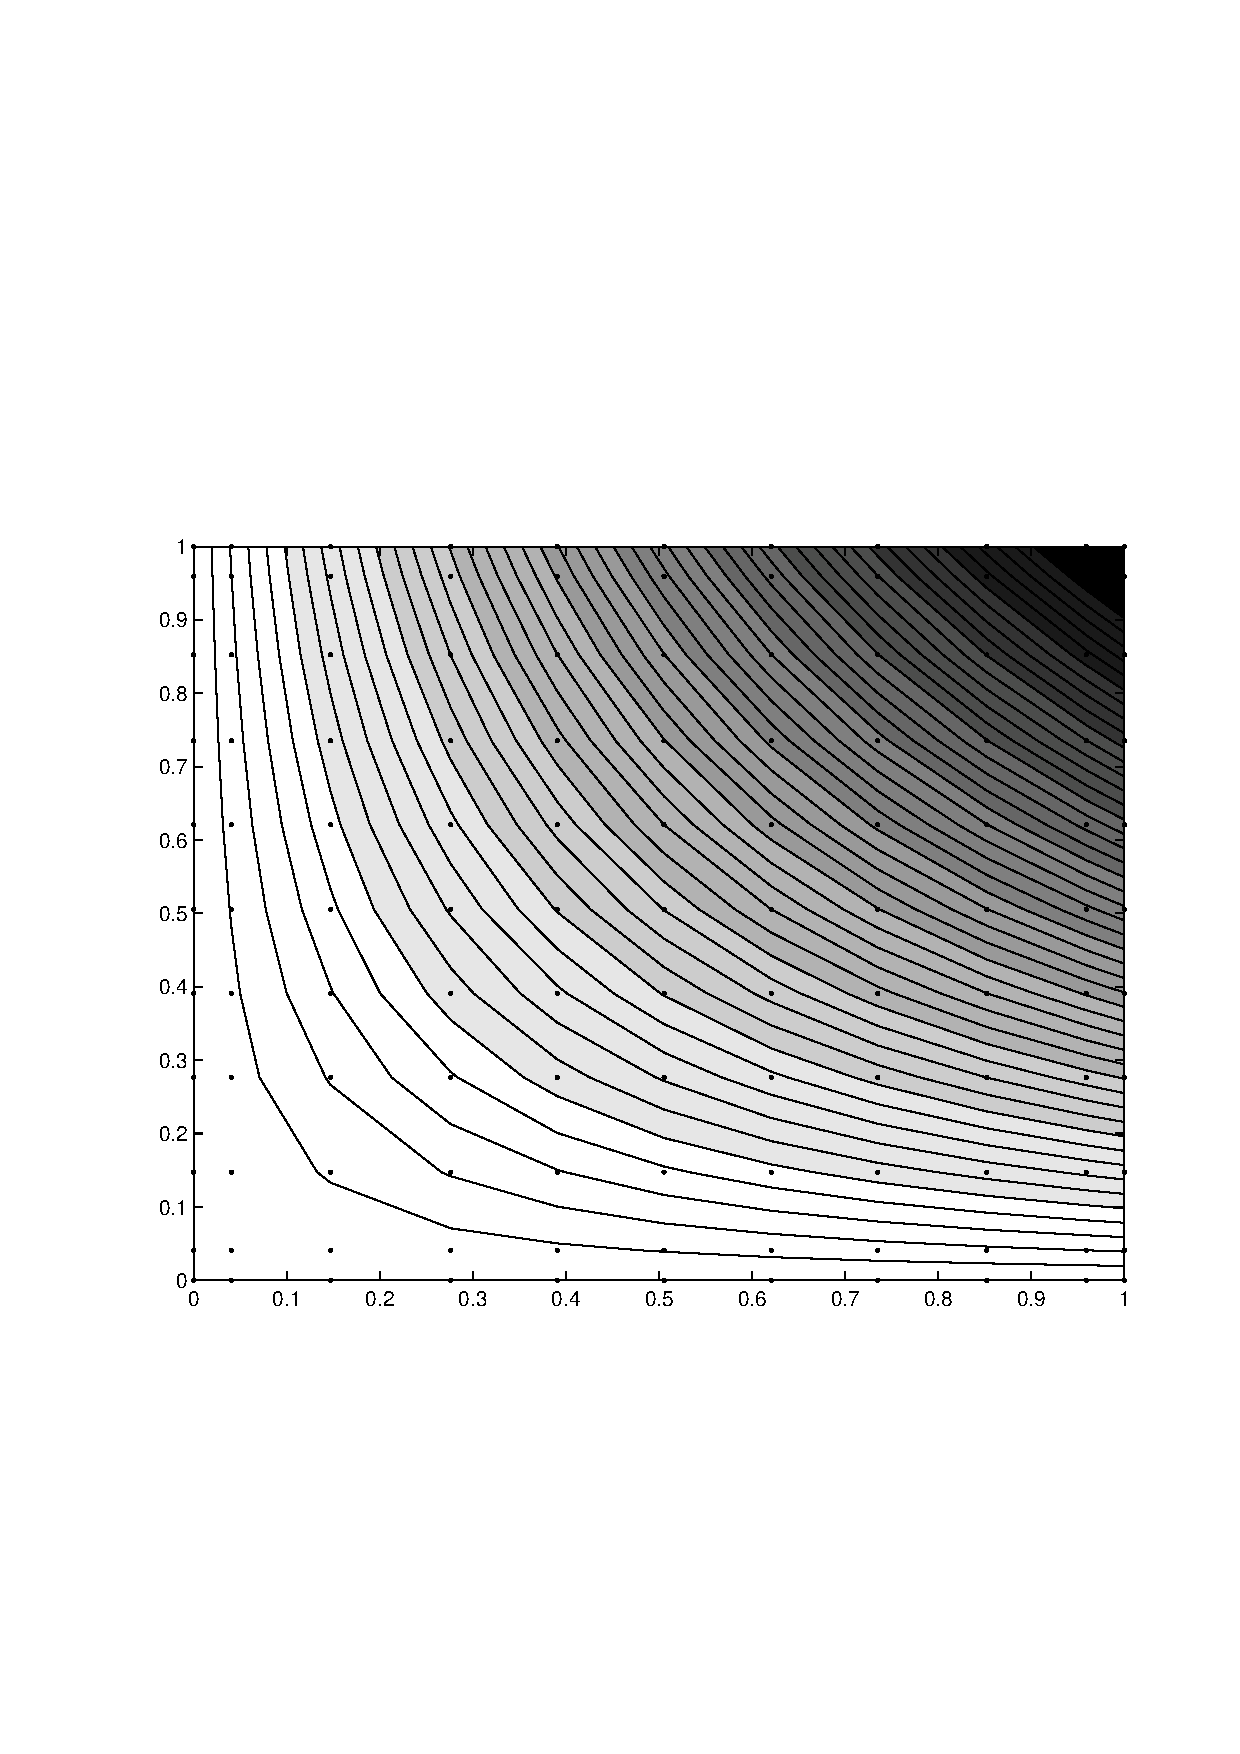
\includegraphics[scale=0.45, trim = 30mm 75mm 15mm 80mm, clip]{./Figures/3-BVP/results_10.pdf}
\caption{Isolines of the $u$ function in the square domain [0,1]x[0,1], 10x10
points.
}
\end{figure}


\columnbreak

\begin{figure}[H]
\centering
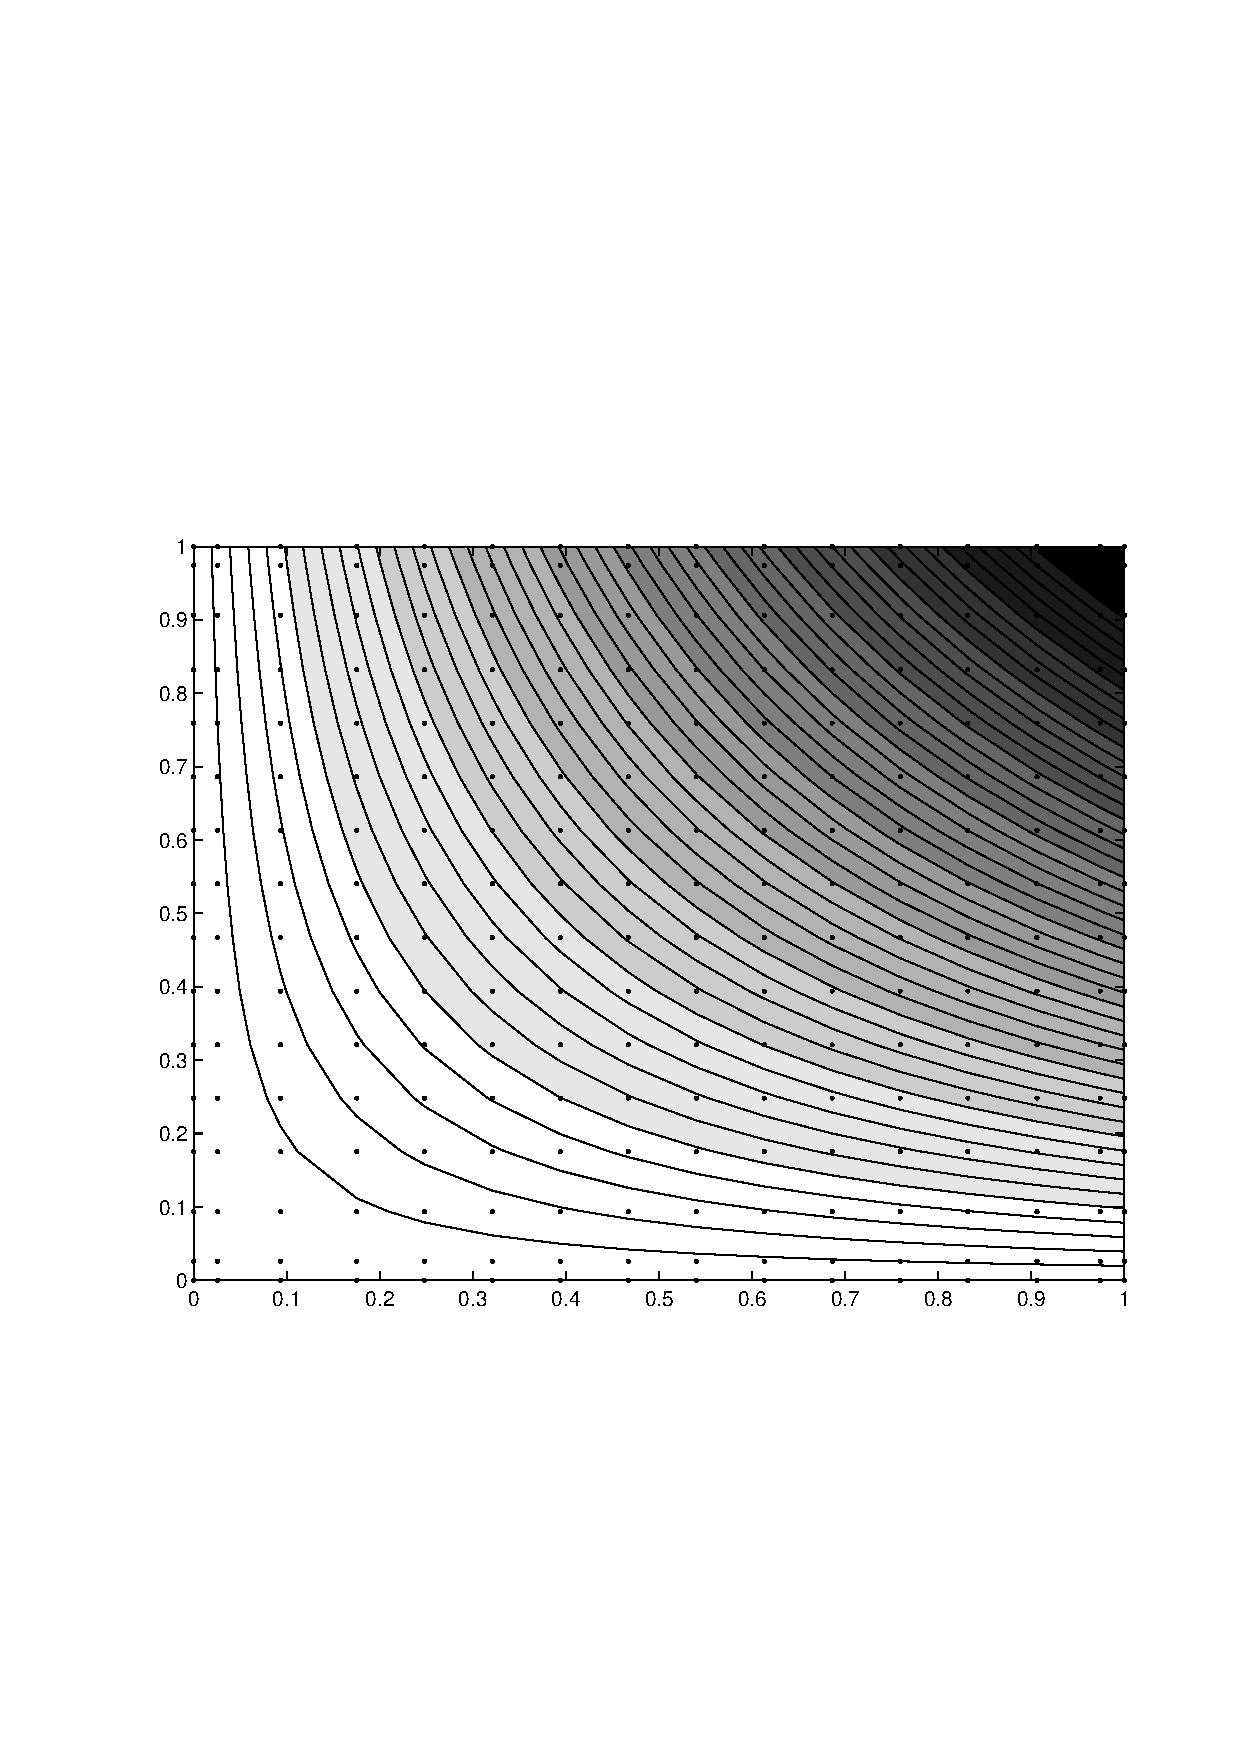
\includegraphics[scale=0.45, trim = 30mm 75mm 15mm 80mm, clip]{./Figures/3-BVP/results_15.pdf}
\caption{Isolines of the $u$ function in the square domain [0,1]x[0,1], 15x15
points. }
\end{figure}

\end{multicols}

\begin{multicols}{2}

\begin{figure}[H]
\centering
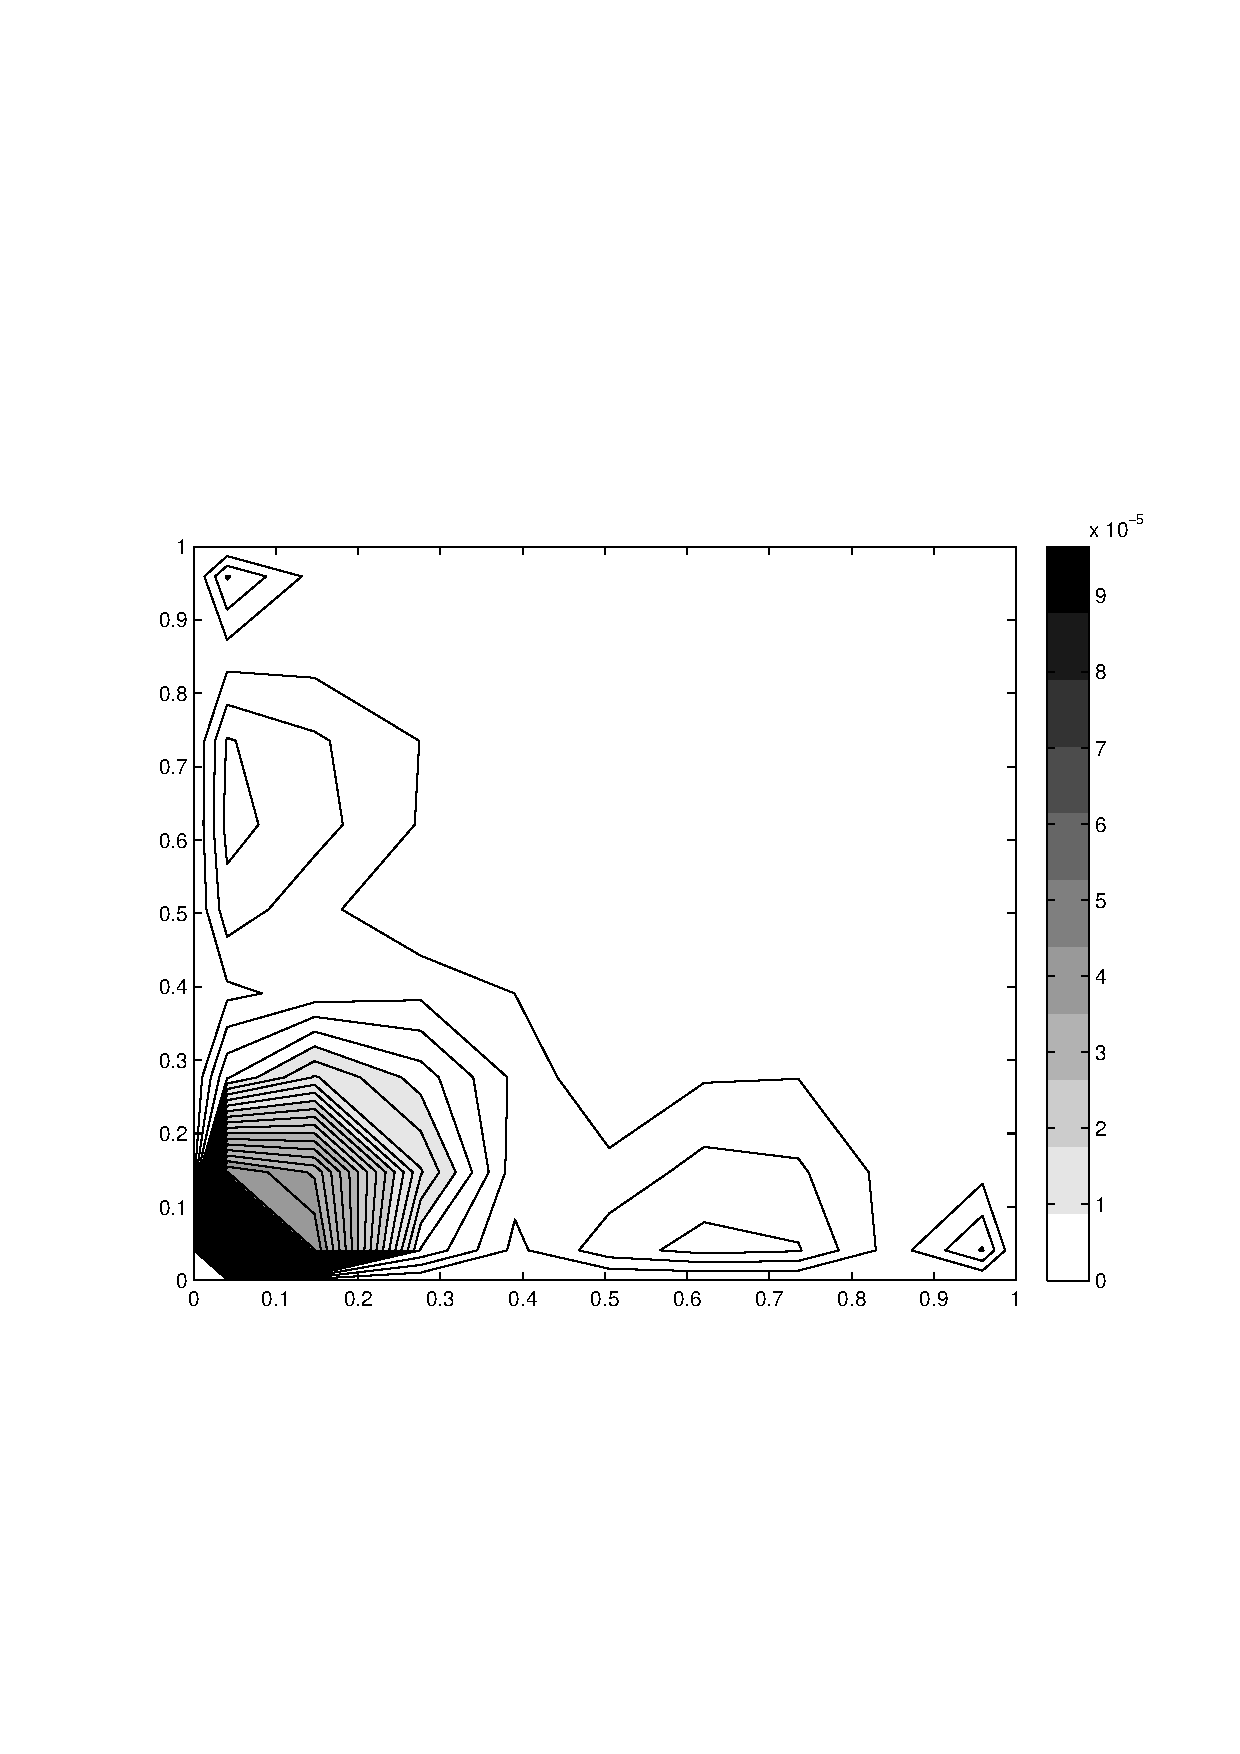
\includegraphics[scale=0.45, trim = 30mm 75mm 15mm 70mm, clip]{./Figures/3-BVP/error_10.pdf}
\caption{Comparison with the exact solution $Error=u_{ij}-x\cdot y$, 10x10
points.}
\end{figure}


\columnbreak

\begin{figure}[H]
\centering
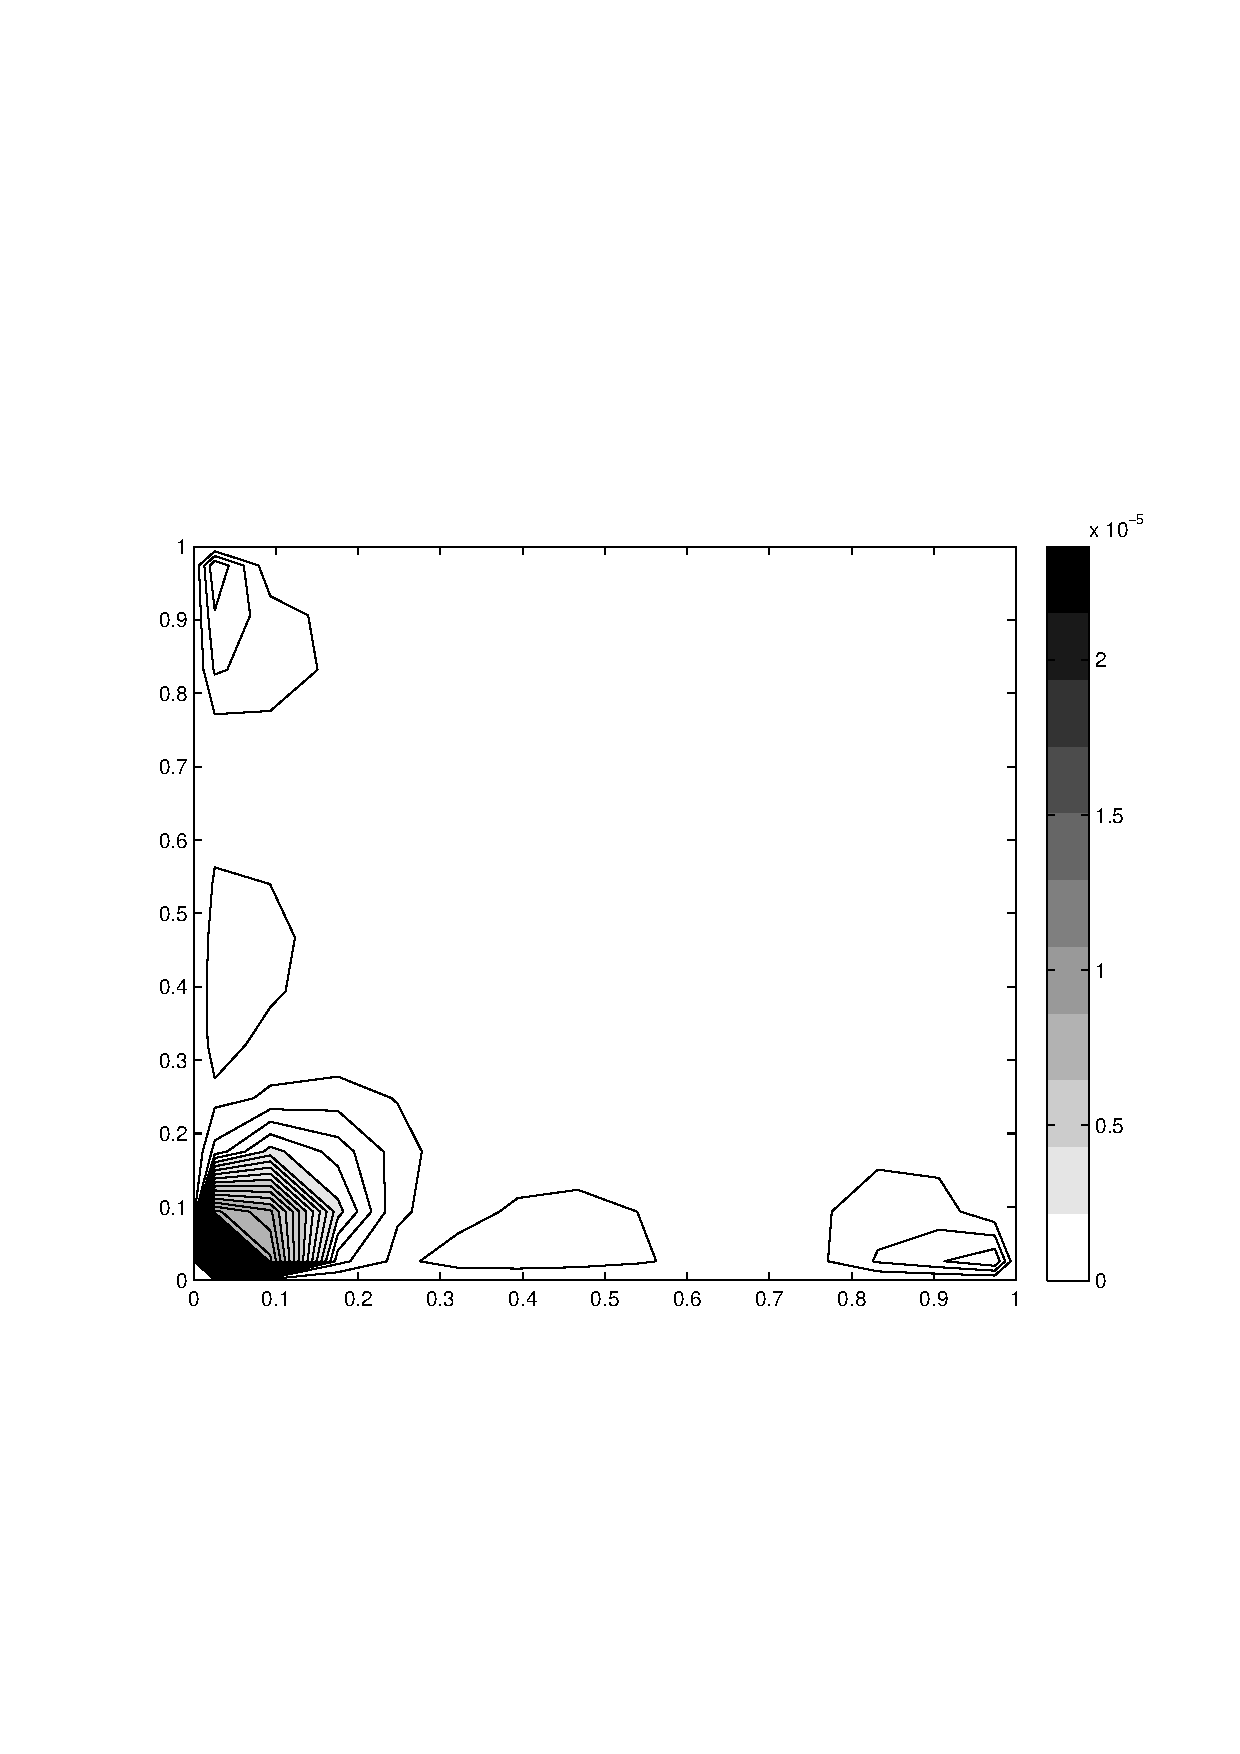
\includegraphics[scale=0.45, trim = 30mm 75mm 15mm 70mm, clip]{./Figures/3-BVP/error_15.pdf}
\caption{Comparison with the exact solution $Error=u_{ij}-x\cdot y$, 15x15
points. }
\end{figure}

\end{multicols}



The software application for this problem is presented now. A good practise
could be to check the solution of the numerical application with different
initial points for the iteration (or even using a different solver defined by
the reader).\\

\begin{blueframed}
\begin{lstlisting}
subroutine Test_non_linear_BVP_4

       use dislin

       integer, parameter :: Nx = 10, Ny = 10
       real :: x(0:Nx), y(0:Ny), U(0:Nx, 0:Ny), err(0:Nx, 0:Ny)

       integer :: i, j
       real :: a=0, b=1
       real :: pi = 4 * atan(1.0)


       x = [ (a + (b-a)*i/Nx, i=0, Nx) ]
       y = [ (a + (b-a)*j/Ny, j=0, Ny) ]

       
        do i=0, Nx
           U(i,:) = 1
     	enddo



      call Non_Linear_Boundary_Value_Problem( x_nodes = x,&
       y_nodes = y, Order =5, Differential_operator = Equation,&
       Boundary_conditions = BCs, Solution = U )

       write(*,*) " maxval, minval y =", maxval(y), minval(y)
       write(*,*) " maxval, minval x =", maxval(x), minval(x)
       write(*,*) " maxval, minval U =", maxval(U), minval(U)
       
       do i=0, Nx
        err(i,:) = x(i)*y(:)-U(i,:)  !numerical vs. analytical
     enddo


       call scrmod('revers')

       call qplcon( U, Nx+1, Ny+1, 20);
        call qplcon( err, Nx+1, Ny+1, 20);

contains

real function Equation(x, y, u, ux, uy, uxx, uyy, uxy)
           real, intent(in) :: x, y, u, ux, uy, uxx, uyy, uxy

        real :: pi = 4 * atan(1.0)

           Equation = (uxx+uyy)*u

end function

real function BCs(x, y, u, ux, uy)
           real, intent(in) :: x, y, u, ux, uy


   if (x==a) then
                      BCs = u
   elseif (x==b) then
                      BCs = u-y
   elseif (y==a) then
                      BCs = u
   elseif (y==b) then
                      BCs = u-x
   else
        write(*,*) " Error BCs x=", x
        write(*,*) " a, b=", a, b
        read(*,*)
   endif

end function

end subroutine

\end{lstlisting}
\end{blueframed}








\newpage
\chapter{Initial Value Boundary Problem}

The previous documents have enlightened how to deal with differential
equation problems, from ordinary to partial derivatives. The idea of this last
document is to go one step further on this scale and give the reader an example
of a mixed problem (it can also be found in the bibliography as 'Initial Value
Boundary Problem'). \\

A mixed problem combines the complexity of Cauchy's and Boundary Value problems,
so one may use the tools and applications described before in order to implement
the software for the new purposes. \\

The description of this problem is presented with an example. Once the example
is understood, one should be able to develop any other problem applying the same
logic and using the software tools available. \\


%1.==========================BODY==============================================
\newpage

\section{Introduction}

The Initial Value Boundary Problem is composed by equations in partial
derivatives which change with time. Usually there is one (or more) parabolic
equation and at least one elliptical equation. Then, the complexity of this
problem mixes the resolution scheme of a Cauchy problem (in order to solve the
temporal evolution) with the procedure for solving a Boundary Problem whose
unknowns change in every time iteration. \\

So, the problem can be written as follows: 

$$\begin{cases}
\frac{d \mathbf{U}}{dt}= \mathbf{F}(\mathbf{U},\mathbf{V}, t) \hspace{1cm} +ICs,
+BCs\\

\mathbf{H}(\mathbf{U},\mathbf{V})=0 \hspace{1.6cm} +BCs\\
\end{cases}
$$

where $\mathbf{U}$ are the unknown variables of the problem with explicit
temporal derivatives and $\mathbf{V}$ are the others (which certainly change
with time but the derivative is not explicit in the equations).
\\

The resolution problem can be summarized as follows: 

Beginning with the initial condition ($\mathbf{U} (t=0)= \mathbf{U_0}$),
$\mathbf{V}$ is calculated from the elliptical equation
$\mathbf{H}(\mathbf{U},\mathbf{V}, t)=0 $. Once $\mathbf{V}$ is known, with the
initial values of $\mathbf{U}$ and $\mathbf{V}$ we are able to evaluate
$\mathbf{F}(\mathbf{U},\mathbf{V})$ and advance one time step using any temporal
scheme. Then the process is restarted with the new $\mathbf{U}$ that has been
calculated. \\

\begin{framed}

\framebox[3cm]{$\begin{array}{c} 
\text{Inital condition},\\
\mathbf{U} (t=0)= \mathbf{U_0} \end{array}$}

\hspace{1.5 cm}$\Downarrow$

\framebox[3cm]{$ \hspace{0.2cm} \begin{cases}
\mathbf{H}(\mathbf{U^n},\mathbf{V})=0
\\
+BCs
\end{cases}$}  
 $\Rightarrow \mathbf{V^n} \Rightarrow $
\framebox[4cm]{$ \hspace{0.2cm} \begin{cases}
\frac{d \mathbf{U}}{dt}= \mathbf{F}(\mathbf{U^n},\mathbf{V^n}, t^n)
\\
+BCs
\end{cases}$}  
 $\Rightarrow \frac{d \mathbf{U^n}}{dt} \Rightarrow $
 \framebox[4cm]{ $\begin{array}{c} 
 
 \text{Temporal scheme}, \\
 
 \mathbf{U^{n+1}}=\mathbf{F}(\mathbf{U^n},\frac{d \mathbf{U^n}}{dt})
 \end{array}$}\\
 
  \hspace{1.5 cm}$\Uparrow$ \hspace{10.5cm} $\Downarrow$
 
\framebox[3cm]{$\mathbf{U^n}$}  \hspace{0.5cm} $\Leftarrow$
\hspace{0.5cm} 
\framebox[4cm]{$t^n = t_0 +n\cdot \Delta t$} 
\hspace{0.5cm} $\Leftarrow$ \hspace{0.5cm}
\framebox[4cm]{$n=n+1$}

\end{framed}

\vspace{1cm}

In order to understand the procedure to solve this kind of problems an example
is presented: the flow inside a square cell, with different temperatures in the
walls. One will see the numerical method (as presented in the chart above) and
some details and particularities which may be interesting in order to show the
capabilities of the software.\\

 In the following section, the problem is presented and then the numerical
 approach to it is explained. \\


\newpage

\section{Convection cell}

The problem presented as example is known in the bibliography as 'Convection
cell'. There is a fluid inside an square box, let's assume the fluid is
incompressible; and the walls may have different boundary conditions. Let one
wall be 'hot' ($T_{hot}$), the opposite one 'cold' ($T_{cold}$) and the two
remaining, adiabatic ($\frac{\delta T}{\delta n}=0$).\\

\begin{figure}[h]
\centering
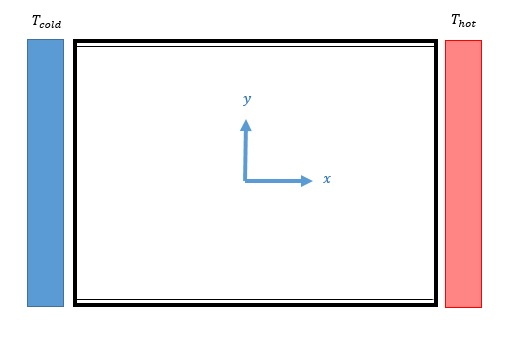
\includegraphics[scale=0.8, trim = 5mm 0mm 0mm 0mm, clip]{./Figures/4-IVBP/figure_0.jpg}
\caption{The convection cell}
\end{figure}

The equations for this problem are: 

\begin {equation} \label{cont}
\nabla \cdot \mathbf{v}= 0
\end{equation}

\begin {equation} \label{cdm}
\rho \cdot \left( \frac{\delta \mathbf {v}}{\delta t} + \mathbf{v} \cdot
\nabla \mathbf{v}\right)= -\nabla P + \mu \cdot \nabla^2 \mathbf{v} + \rho g
\beta T (-\mathbf{j})
\end{equation}

\begin {equation} \label{ener}
\rho c_p \cdot \left( \frac{\delta T}{\delta t} + \mathbf{v} \cdot
\nabla T\right)= k \cdot \nabla^2 T + q
\end{equation}

The first difficulty to solve this problem is the boundary condition in the
pressure field ($P$), which is not evident. An alternative path to this problem
is working in terms of the stream function \ref{stream_function} and
vorticity \ref{vorticity}. \\

\begin {equation} \label{stream_function}
u=\frac{\delta \Psi}{\delta y}, \hspace{0.5cm} v=-\frac{\delta \Psi}{\delta x},
\end{equation}

\begin{equation} \label{vorticity}
\omega= \nabla \times \mathbf{v}
\end{equation}

Then, the equations \ref{vorticity} and \ref{cdm} can be written as follows
\footnote{The continuity equation is no longer needed because the stream function ensures its compliance.}:

\begin {equation} \label{cont2}
\omega= - \nabla^2 \Psi
\end{equation}

\begin {equation} \label{cdm2}
\rho \cdot \left( \frac{\delta \omega}{\delta t} + \mathbf{v} \cdot
\nabla \omega\right)=  \mu \cdot \nabla^2 \omega - \rho g
\beta \frac{\delta T}{\delta x}
\end{equation}

With this new approach, the unknown functions of the problem are scalar
fields (in fact the vorticity is vectorial but in a 2D problem only the normal
component plays a roll in the flow), the boundary conditions can be imposed on
the stream function and temperature and the pressure is hidden in this
formulation. \\

A second difficulty appears however, once again concerning the boundary
conditions. As we are to solve the problem inside a closed box, the velocity of
the fluid is assumed zero for the fluid in contact with the walls. These
boundary conditions lead to eight equations in the stream function ($u=v=0$ in
$\delta \Omega$, that is to say in each of the four walls), while there is no
boundary condition in the vorticity. This difficulty will be dealed later when
explaining the numerical approach to the problem. \\

\vspace{1 cm}

So, for this problem three equations are needed \ref{cont2}, \ref{cdm2},
\ref{ener}, for the three scalar fields $\Psi$, $\Omega$ and $T$. Plus, one
can also compute the velocity from the definition of the stream function
\ref{stream_function}, but this is not essential. \\

Now, as usual when working with fluids, let's transform the equations to
non-dimensional variables. \\



\subsection{Non-dimensional equations}

First of all some magnitudes are to be defined: 

\begin{itemize}
  \item Characteristic dimension: the length of the walls $2a$: $x=(2a)\hat x$, 
  $y=(2a)\hat y$.
  \item Characteristic velocity $u_c$ \footnote{Sometimes, in this kind of problems the
  characteristic velocity is written as $u_c= \frac{k}{\rho c_p (2a)}$, which
  is useful for simplifying  the problem.}: $u= u_c \cdot \hat u$, $v=
  u_c \cdot \hat v$ .
  \item Temperature $\theta= \frac{T-T_{cold}}{T_{hot}-T_{cold}}$.
  \item Time $t= \frac{(2a)}{u_c} \hat t$
\end{itemize}

and three characteristic numbers appears: 

\begin{itemize}
  \item Reynolds $Re \sim \frac{\rho u_c (2a)}{\mu}$ \footnote{If $u_c=
  \frac{k}{\rho c_p (2a)}$, then $Re \sim 1/Pr$}.
  
  \item Prandtl $Pr \sim \frac{\mu c_p}{k}$.
  \item Rayleigh $Ra \sim \frac{g \beta (T_{hot}-T_{cold})}{\frac{\mu}{\rho}
  \frac{k}{\rho c_p}}\cdot (2a)^3$
\end{itemize}

So the equations are: 

\begin {equation} \label{cont3}
\omega= - \left( \frac{\delta^2 \Psi}{\delta x^2} + \frac{\delta^2
 \Psi}{\delta y^2} \right)
\end{equation}

\begin {equation} \label{cdm3}
 \frac{\delta \omega}{\delta t} = -u \cdot \frac{\delta \omega}{\delta x} -v
 \cdot \frac{\delta \omega}{\delta y} +
 \frac{1}{Re} \cdot \left( \frac{\delta^2 \omega}{\delta x^2} + \frac{\delta^2
 \omega}{\delta y^2} \right) - \frac{Ra}{Pr \cdot Re^2}
\frac{\delta \theta}{\delta x}
\end{equation}

\begin {equation} \label{ener3}
 \frac{\delta \theta}{\delta t} =  -u \cdot \frac{\delta \theta}{\delta x} -v
 \cdot \frac{\delta \theta}{\delta y}+ \frac{1}{Re \cdot Pr} \cdot \left(
 \frac{\delta^2 \theta}{\delta x^2} + \frac{\delta^2 \theta}{\delta y^2} \right)
\end{equation}


Where all the variables are non-dimensional ( $\hat{\phi}$ has been omitted for
simplifying the writing).

\subsection{Boundary conditions}

We have pointed that there is a difficulty concerning the boundary conditions.
As we have said, eight boundary conditions applies to the stream function while
no condition is applied to the vorticity. \\

The conditions for the stream function comes from assuming zero velocity of the
fluid in contact with the walls. Then, 

\begin{equation}
u(x,y)=v(x,y)=0, \hspace{1cm} (x,y)\in \delta \Omega
\end{equation}

\begin{equation}
\frac{\delta \Psi}{\delta y} (x,y)= \frac{\delta \Psi}{\delta x} (x,y)=0,
\hspace{1cm} (x,y)\in \delta \Omega
\end{equation}

It can also be written as follows: 

\begin{equation}
\frac{\delta \Psi}{\delta \mathbf{s}} (x,y)= \frac{\delta \Psi}{\delta
\mathbf{n}} (x,y)=0, \hspace{1cm} (x,y)\in \delta \Omega
\end{equation}

Where $\mathbf{s}$ and $\mathbf{n}$ are the coordinates along the wall and
normal to it, respectively.\\

The boundary conditions for the temperature can be arbitrary. One can choose
two walls with different temperatures and the remaining ones, adiabatic:

\begin{equation}
T=T_{cold} \rightarrow \theta=0, \hspace{1cm}
(x,y)\in(-a,y)
\end{equation}

\begin{equation}
T=T_{hot} \rightarrow \theta=1, \hspace{1cm}
(x,y)\in(+a,y)
\end{equation}

\begin{equation}
\frac{\delta T}{\delta \mathbf{n}}=0 \rightarrow \frac{\delta \theta}{\delta
\mathbf{n}}=0, \hspace{1cm} (x,y)\in(x,\pm b)
\end{equation}\\ 

\begin{figure}[h]
\centering
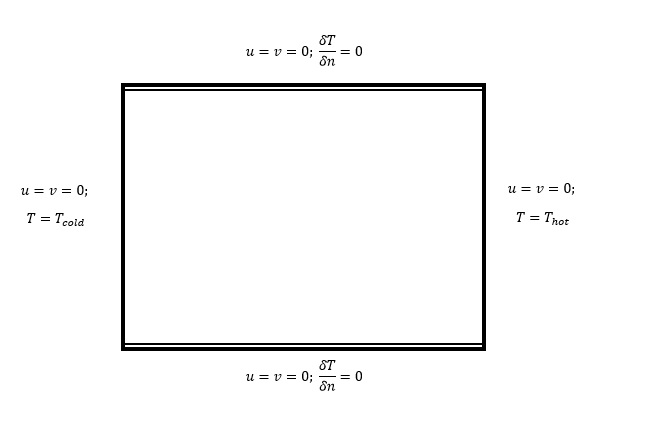
\includegraphics[scale=0.8, trim = 5mm 10mm 0mm 10mm,
clip]{./Figures/4-IVBP/figure_1.jpg}
\caption{Spatial domain and boundary conditions}
\label{BC_figure}
\end{figure}

The boundary conditions for the vorticity will be taken from the equation
\ref{cont3} once the stream function is known. The solving process can be
summarized as follows: 

\begin{itemize}
  \item Assuming the vorticity is known in the interior points of the domain (at
  the beginning from the initial condition and then from the previous time step), the stream function is
  calculated with \ref{cont3}: 
$$ \omega= - \left( \frac{\delta^2 \Psi}{\delta x^2} + \frac{\delta^2
 \Psi}{\delta y^2} \right) \rightarrow \Psi=\Psi(x,y)$$
 \item Then, the vorticity in the boundaries of the spatial domain is calculated
 with this same equation: 
 $$ \omega_{\delta \Omega}= - \left( \frac{\delta^2 \Psi}{\delta
 x^2} + \frac{\delta^2 \Psi}{\delta y^2} \right)_{\delta \Omega} \rightarrow
 \omega_{\delta \Omega}=\omega(x,y) \hspace{0.5cm} (x,y) \in \delta \Omega$$
 \item These values are used as boundary conditions for the evolution problem
 (equation \ref{cdm3}).
\end{itemize} 


Now, let's look into the numerical approach to this problem. \\

\newpage

\section{Numerical approach to the problem}

First of all the equations will be discretized. The notation we have used is: 

$$\theta(x,y,t) \rightarrow \theta^{ij} = \theta(i,j)_n$$

Where $i,j$ are the index of the spatial mesh ($x_i, y_j$) and $n$ refers to the
time step ($t=t_0+n\cdot \Delta t$). \\

The discretized equations are: 

\begin {equation} \label{cont4}
\omega^{ij}= - (\Psi^{ij} _{xx} + \Psi^{ij} _{yy})
\end{equation}

\begin {equation} \label{cdm4}
 \frac{\delta \omega^{ij}}{\delta t} = -\Psi^{ij} _{y} \cdot 
 \omega^{ij}_x + \Psi^{ij} _{x} \cdot \omega^{ij}_y +
 \frac{1}{Re} \cdot ( \omega^{ij}_{xx} + \omega^{ij}_{yy}) - \frac{Ra}{Pr \cdot
 Re^2} \cdot \theta^{ij}_x
\end{equation}

\begin {equation} \label{ener4}
 \frac{\delta \theta^{ij}}{\delta t} =  -\Psi^{ij} _{y} \cdot 
 \theta^{ij}_x + \Psi^{ij} _{x} \cdot \theta^{ij}_y + \frac{1}{Re \cdot Pr}
 \cdot ( \theta^{ij}_{xx} + \theta^{ij}_{yy})
\end{equation}

The boundary conditions: 

\begin{equation} \label{BCs1}
 \Psi^{ij}_ \mathbf{s}= \Psi^{ij}_ \mathbf{n}=0, \hspace{1cm} (i,j)\in \delta
 \Omega
\end{equation}

\begin{equation} \label{BCs2}
 \omega^{ij} = f(\Psi^{ij}), \hspace{1cm} (i,j)\in \delta
 \Omega
\end{equation}

\begin{equation} \label{BCs3}
 \theta^{ij}_ \mathbf{n}=0, \hspace{1cm} (i,j)\in
 \delta \Omega_0
\end{equation}

\begin{equation} \label{BCs4}
 \theta^{ij} =0, \hspace{1cm} (i,j)\in
 \delta \Omega_1
\end{equation}

\begin{equation} \label{BCs5}
 \theta^{ij} =1, \hspace{1cm} (i,j)\in
 \delta \Omega_2
\end{equation}

And the initial conditions: 

\begin{equation} \label{IC1}
 \omega^{ij} = \omega^{ij}_0, \hspace{1cm} (i,j)\in  \Omega
\end{equation}

\begin{equation} \label{IC2}
 \theta^{ij} = \theta^{ij}_0, \hspace{1cm} (i,j)\in  \Omega
\end{equation}

\subsection{Solving procedure}

\begin{framed}

\framebox[3cm]{$\begin{array}{c} 
\text{Inital condition},\\
\omega^{ij}_0  \hspace{0.5cm}\text{eq. [\ref{IC1}]}\end{array}$}

\hspace{1.5 cm}$\Downarrow$

\framebox[3cm]{$ \hspace{0.2cm} \begin{cases}
\text{BVP eq.[\ref{cont4}]}\\
\text{+ BCs eq.[\ref{BCs1}]}
\end{cases}$}  
 $\Rightarrow \Psi^{ij} \Rightarrow $
\framebox[4cm]{$ \hspace{0.2cm} \begin{cases}
\text{Cauchy  eq.[\ref{cdm4} \ref{ener4}] }\\
\text{+ BCs eq.[\ref{BCs2} \ref{BCs3} \ldots]}
\end{cases}$}  
 $\Rightarrow \frac{d \mathbf{U^n}}{dt} \Rightarrow $
 \framebox[4cm]{ $\begin{array}{c} 
 
 \text{Temporal scheme}, \\
 
 \mathbf{U^{n+1}}=\mathbf{F}(\mathbf{U^n},\frac{d \mathbf{U^n}}{dt})
 \end{array}$}\\
 
  \hspace{1.5 cm}$\Uparrow$ \hspace{10.5cm} $\Downarrow$
 
\framebox[3cm]{$\mathbf{\omega_{n}^{ij}}$}  \hspace{0.5cm}$\Leftarrow$
\hspace{0.5cm} \framebox[4cm]{$t^n = t_0 +n\cdot \Delta t$} 
\hspace{0.5cm} $\Leftarrow$ \hspace{0.5cm}
\framebox[4cm]{$n=n+1$}


\end{framed}


\newpage
\subsection{Boundary value problem}

As we have seen, with the vorticity field from the previous iteration we can
solve the boundary value problem and find the new stream function. The equations
are: 

\begin {equation} \label{cont4}
\omega^{ij}= - (\Psi^{ij} _{xx} + \Psi^{ij} _{yy})
\end{equation}

\begin{equation} \label{BCs10}
 \Psi^{ij}_ \mathbf{s}= \Psi^{ij}_ \mathbf{n}=0, \hspace{1cm} (i,j)\in \delta
 \Omega
\end{equation}

The important thing to remark here is that eight conditions are to be applied
while only four are necessary to solve the Poisson problem. As we have explained
this is because there are four of this conditions that substitute the unknown
boundary conditions of the vorticity. \\

In order to solve this problem, first of all let's look into the discretized
boundary conditions using finite differences as usual. Then, the derivative is
transformed to a polynomial expression depending on the function value of the
nearby points. For example in the wall at $x=-a$ ($i=0$):

\begin{equation} \label{BCs101}
 \Psi^{0,j}_ \mathbf{s} = f(\Psi^{0,j-n} \ldots \Psi^{0,j} \ldots \Psi^{0,j+n}
 )=0
\end{equation}

\begin{equation} \label{BCs102}
 \Psi^{0,j}_ \mathbf{n} = f(\Psi^{0,j}, \Psi^{1,j} \ldots \Psi^{n,j} )=0
\end{equation}\\

\begin{figure}[h]
\centering
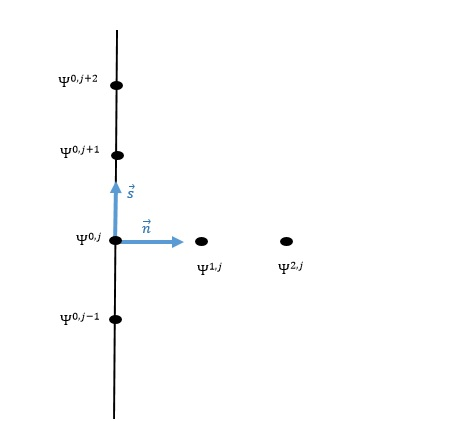
\includegraphics[scale=1, trim = 5mm 0mm 30mm 10mm,
clip]{./Figures/4-IVBP/figure_2.jpg}
\caption{Boundary conditions for the stream function}
\label{BC_figure_2}
\end{figure}


The equations \ref{BCs101} and \ref{BCs102} can be rewritten as follows: 

\begin{equation} \label{BCs103}
 \Psi^{0,j} = f(\Psi^{0,j-n} \ldots \Psi^{0,j+n})
\end{equation}

\begin{equation} \label{BCs104}
 \Psi^{1,j}= f(\Psi^{0,j}  \ldots \Psi^{n,j} )
\end{equation}\\

Proceeding the same way in the other walls we will get enough equations for the
function values in the boundary points and the following ones. Then, the Poisson
problem is to be solved in the interior points (inside the dashed square in the
figure):

\begin {equation} \label{cont5}
\omega^{ij}= - (\Psi^{ij} _{xx} + \Psi^{ij} _{yy}) \hspace{1cm} (i,j) \in
(2:Nx-2, 2:Ny-2)
\end{equation}

\begin{figure}[h]
\centering
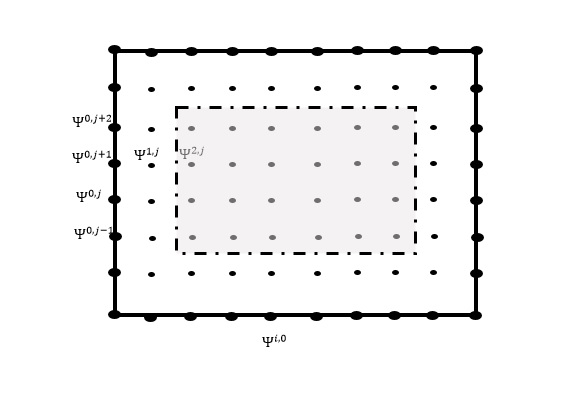
\includegraphics[scale=1, trim = 5mm 10mm 10mm 0mm, clip]{./Figures/4-IVBP/figure_3.jpg}
\caption{Boundary value problem}
\label{BVP}
\end{figure}

For this purpose a special extension of the boundary value problem application
has been prepared. This subroutine allows the user to work with the two boundary
conditions in each wall while the differential equation is applied only in a
square of dimension $(2:N-2)\times(2:N-2)$: 

\begin{blueframed}
\begin{lstlisting}
subroutine multiBC_Boundary_Value_Problem2D(x_nodes, y_nodes, &
		Order, Differential_operator, &
		Boundary_conditions1, Boundary_conditions2, &
		Solution)

     real, intent(inout) :: x_nodes(0:), y_nodes(0:)
     integer, intent(in) :: Order
     procedure (DifferentialOperator2D) :: Differential_operator
     procedure (BC2D) ::  Boundary_conditions1
     procedure (BC2D) ::  Boundary_conditions2
     real, intent(out) :: Solution(:,:)

\end{lstlisting}
\end{blueframed}

However, from the application layer the user should call the routine as usual
just applying two sets of boundary conditions (the easiest way is to define the
conditions on $s$ in one function and the ones in $n$ in a different one).\\

\begin{blueframed}
\begin{lstlisting}
call Boundary_Value_Problem(x_nodes= x_nodes, y_nodes= y_nodes,&
		 Order = Order, &
                 Differential_operator = Equation,  &
                 Boundary_conditions1 = BCs1, &
                 Boundary_conditions2 = BCs2, Solution = FF )
\end{lstlisting}
\end{blueframed}


\begin{blueframed}
\begin{lstlisting}
real function BCs1(x, y, u, ux, uy)
           real, intent(in) :: x, y, u, ux, uy


   if (x==x_nodes(0)) then
                      BCs1 = uy
   elseif (y==y_nodes(0)) then
                      BCs1 = ux
   elseif (x==x_nodes(Nx)) then
                      BCs1 = uy
   elseif (y==y_nodes(Ny)) then
                      BCs1 = ux
   else
        write(*,*) " Error BCs x=", x
        write(*,*) " a, b=", a, b
        read(*,*)
   endif

end function

real function BCs2(x, y, u, ux, uy)
           real, intent(in) :: x, y, u, ux, uy


   if (x==x_nodes(0)) then
                      BCs2 = ux
   elseif (y==y_nodes(0)) then
                      BCs2 = uy
   elseif (x==x_nodes(Nx)) then
                      BCs2 = ux
   elseif (y==y_nodes(Ny)) then
                      BCs2 = uy
   else
        write(*,*) " Error BCs x=", x
        write(*,*) " a, b=", a, b
        read(*,*)
   endif

end function
\end{lstlisting}
\end{blueframed}

\subsection{Cauchy Problem}

The boundary condition for the vorticity is calculated from the stream function: 

\begin {equation} \label{BCs200}
\omega^{ij}= - (\Psi^{ij} _{xx} + \Psi^{ij} _{yy}) \hspace{1cm} (i,j)\in \delta \Omega
\end{equation}

And the evolution problem for the interior points is to be written as usual,
with the equations \ref{cdm4}, \ref{ener4}:

\begin {equation} \label{Cauchy}
\frac{d \mathbf{X}}{dt}= \mathbf{F} (\mathbf{X}) 
\end{equation}

\begin {equation} \label{Cauchy2}
\frac{d}{dt} \left \{ {\begin{array}{c} \omega^{ij} \\ \theta^{ij} \end{array}}
\right \}= \left \{ {\begin{array}{c} F_{xy} (\omega^{ij}, \Psi^{ij},
\theta^{ij}) \\
T_{xy}(\Psi^{ij}, \theta^{ij})
\end{array}} \right \}
\end{equation}


So a transformation is needed from the matrix $\omega^{ij}$, $\theta^{ij}$ to the vector $X$: 

\begin{blueframed}
\begin{lstlisting}
	X(1:M)=reshape(WW, [ M ]);
	X(M+1:2*M)=reshape(TT, [ M ]);
\end{lstlisting}
\end{blueframed}

Where $M$ is the total amounts of nodes: $M=(N_x+1)\cdot(N_y+1)$. \\

However it is more comfortable to us to work with $WW(i,j)$ and $TT(i,j)$ rather
than $X(k)$. So each time step we will transform the vector, calculate the
operator $F$ and then return this operator with the appropriate structure: 

\begin{blueframed}
\begin{lstlisting}
	WW = reshape( X(1:M), [Nx+1, Ny+1] )
	TT = reshape ( X(M+1:2*M), [Nx+1, Ny+1] )
	
	!call BVP for the stream function
	!...(calculation of the operator F)
	
	F(1:M)=reshape(Fxy, [ M ] );
	F(1+M:2*M)=reshape(Txy, [ M ] );
\end{lstlisting}
\end{blueframed}


\begin{blueframed}
\begin{lstlisting}
 call Cauchy_Problem_Solution( Domain = T_Domain, &
 		Initial_C = vorticity_IC, &
		System = System_1, &
		Scheme= Runge_Kutta4, &
		Outputs = vorticity_graphs)
\end{lstlisting}
\end{blueframed}

\newpage

\section{Results}

With the aim of testing the application, a model is prepared with the following
parameters:

$$\text{Characteristic velocity:   }\hspace{0.5cm} u\sim \frac{k}{\rho c_p
(2a)}$$ $$\text{Reynolds number:   }\hspace{0.5cm} Re= \frac{\rho u (2a)}{\mu} \sim
\frac{1}{Pr}
$$
$$\text{Prandtl number:   }\hspace{0.5cm} Pr= \frac{\mu c_p }{k} \sim 1
$$
$$\text{Rayleigh number:   }\hspace{0.5cm} Ra= \frac{g \beta
(T_{hot}-T_cold)}{\frac{\mu}{\rho} \frac{k}{\rho c_p}} (2a)^3 \sim 10^5 $$


The following figures present the results obtained of the test case.

\begin{multicols}{2}

\begin{figure}[H]
\centering
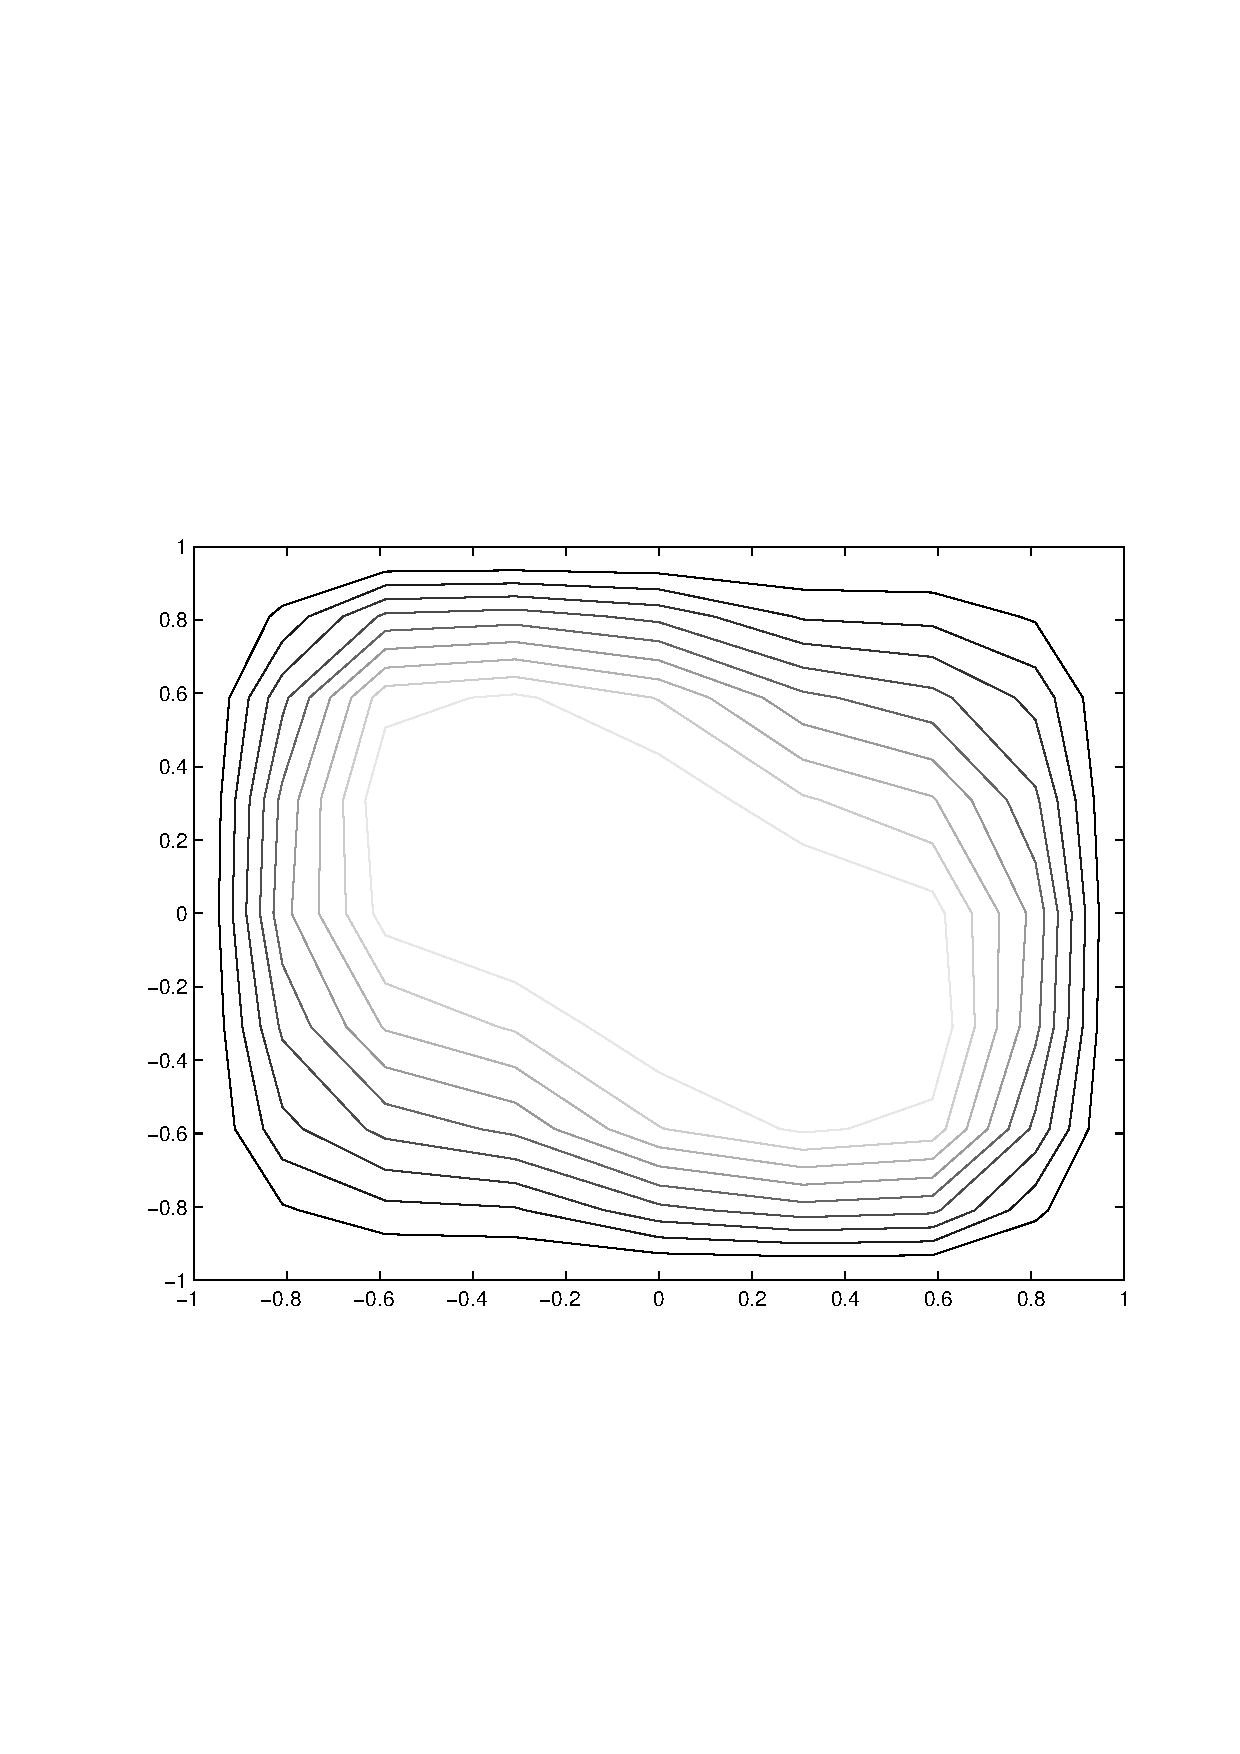
\includegraphics[scale=0.45, trim = 30mm 75mm 15mm 80mm, clip]{./Figures/4-IVBP/stream_t_1.pdf}
\caption{Stream function isolines, $t=0.1$.
}
\end{figure}


\columnbreak

\begin{figure}[H]
\centering
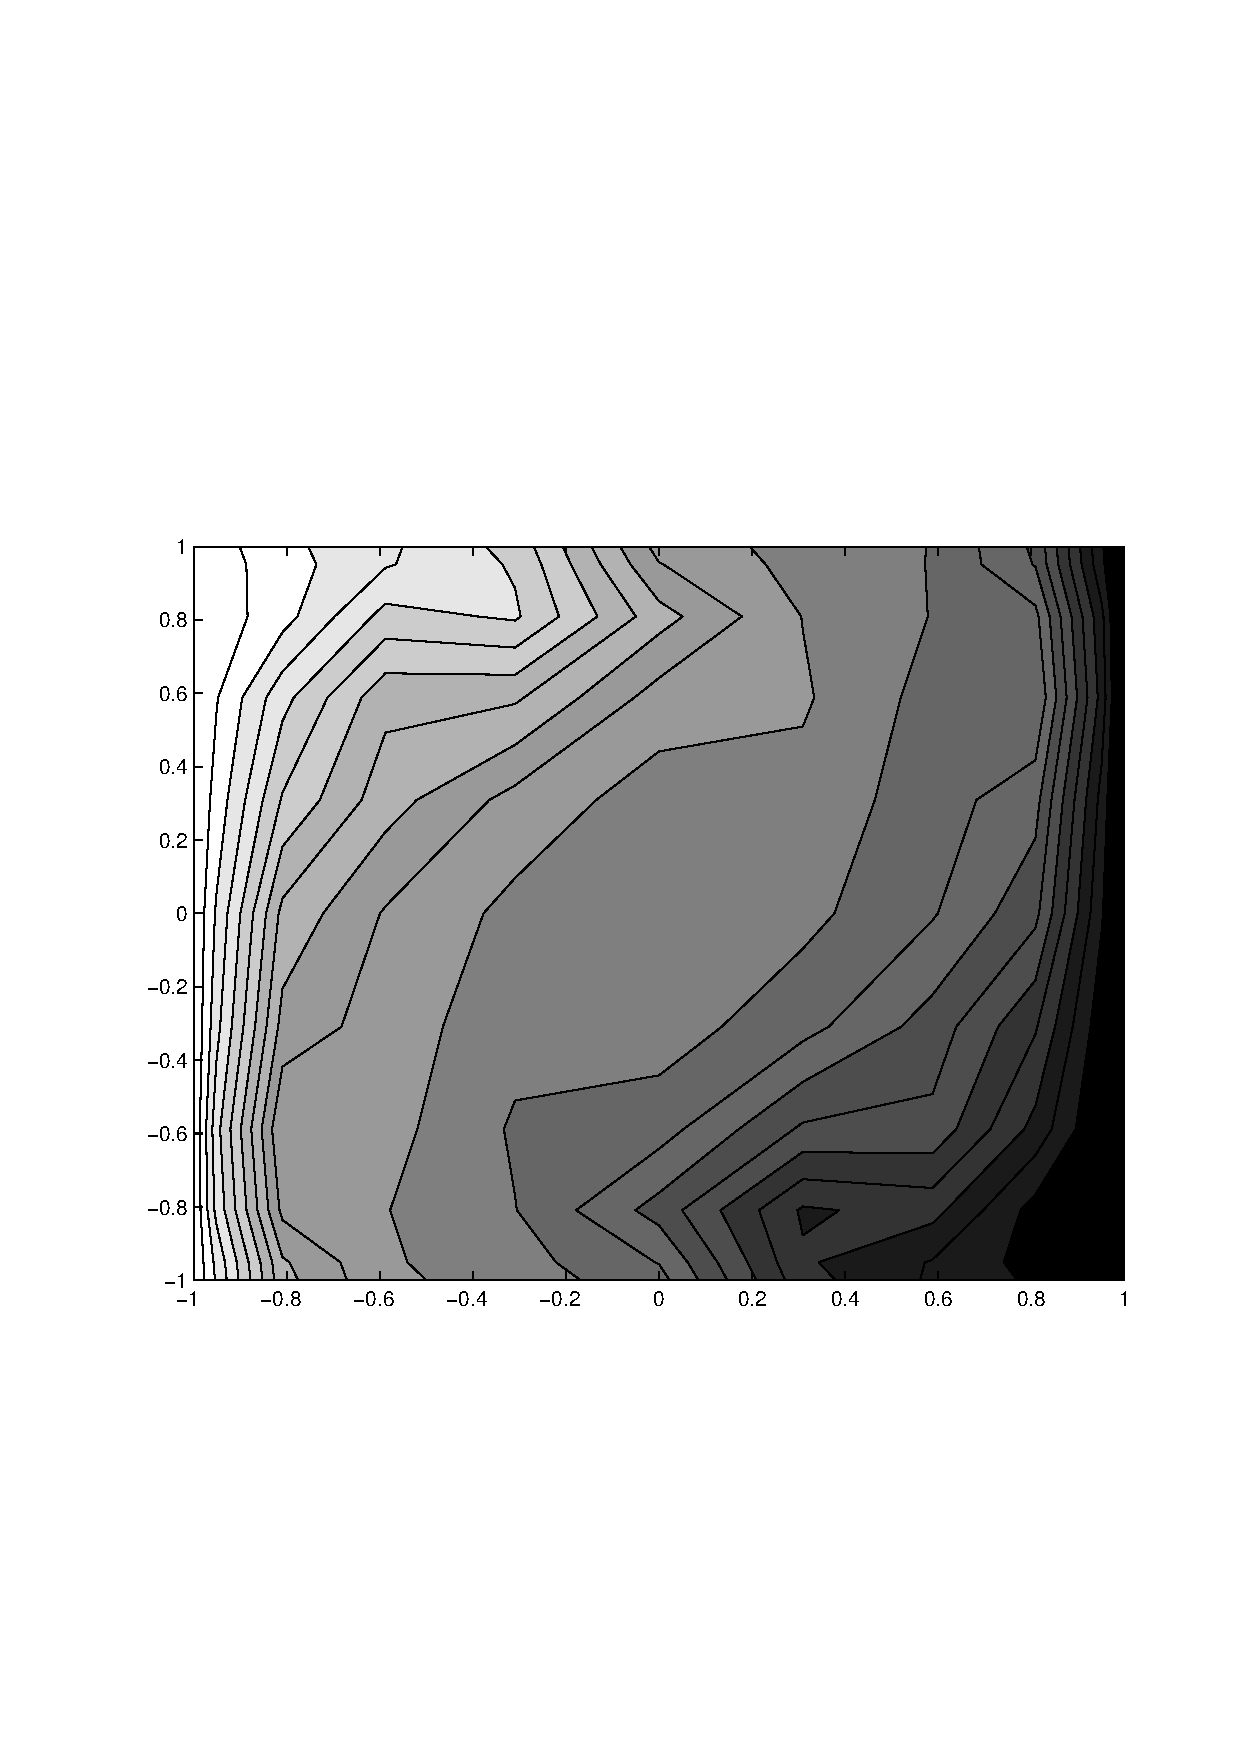
\includegraphics[scale=0.45, trim = 30mm 75mm 15mm 80mm,
clip]{./Figures/4-IVBP/temperature_t_1.pdf} \caption{Temperature contours, $t=0.1$.}
\end{figure}

\end{multicols}

\begin{multicols}{2}

\begin{figure}[H]
\centering
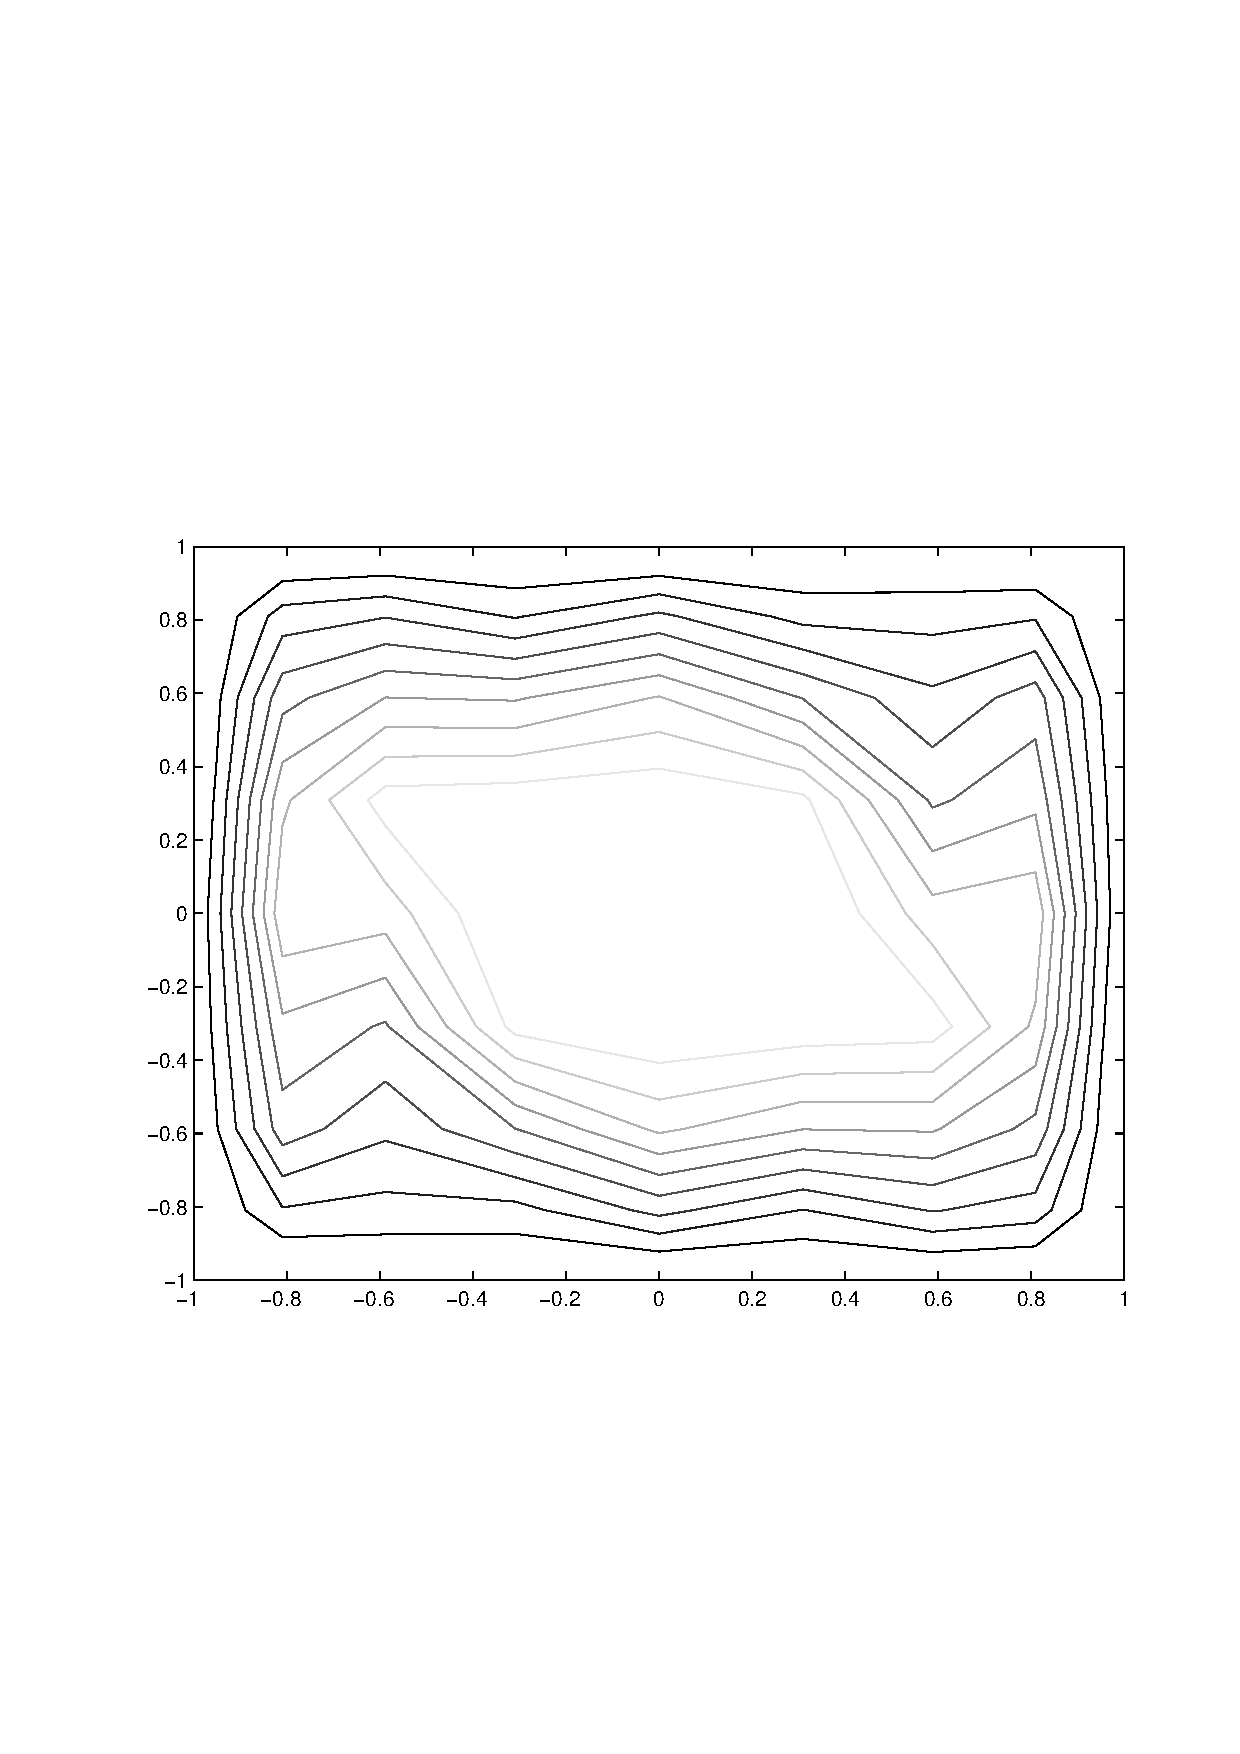
\includegraphics[scale=0.45, trim = 30mm 75mm 15mm 80mm, clip]{./Figures/4-IVBP/stream_t_5.pdf}
\caption{Stream function isolines, $t=0.5$.
}
\end{figure}


\columnbreak

\begin{figure}[H]
\centering
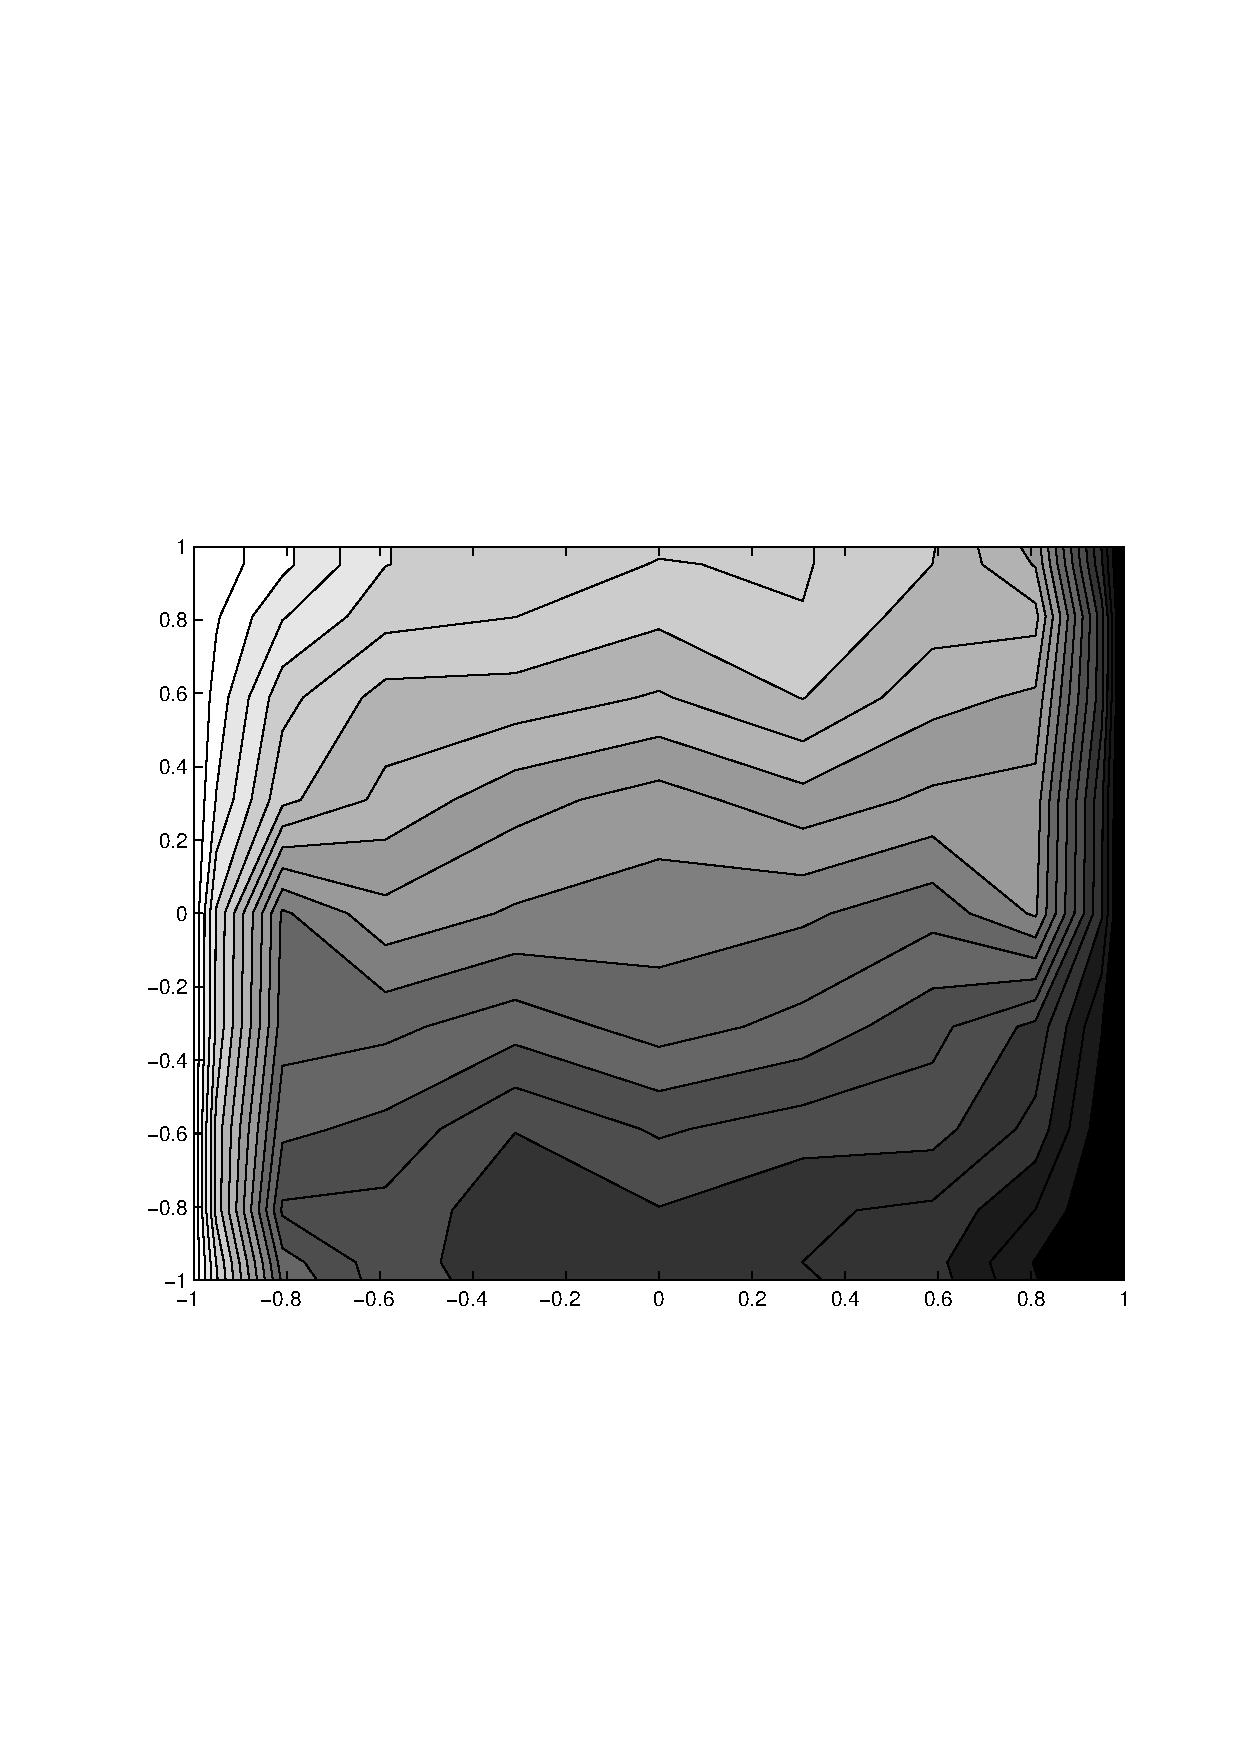
\includegraphics[scale=0.45, trim = 30mm 75mm 15mm 80mm,
clip]{./Figures/4-IVBP/temperature_t_5.pdf} \caption{Temperature contours, $t=0.5$.}
\end{figure}

\end{multicols}

\newpage

\begin{multicols}{2}

\begin{figure}[H]
\centering
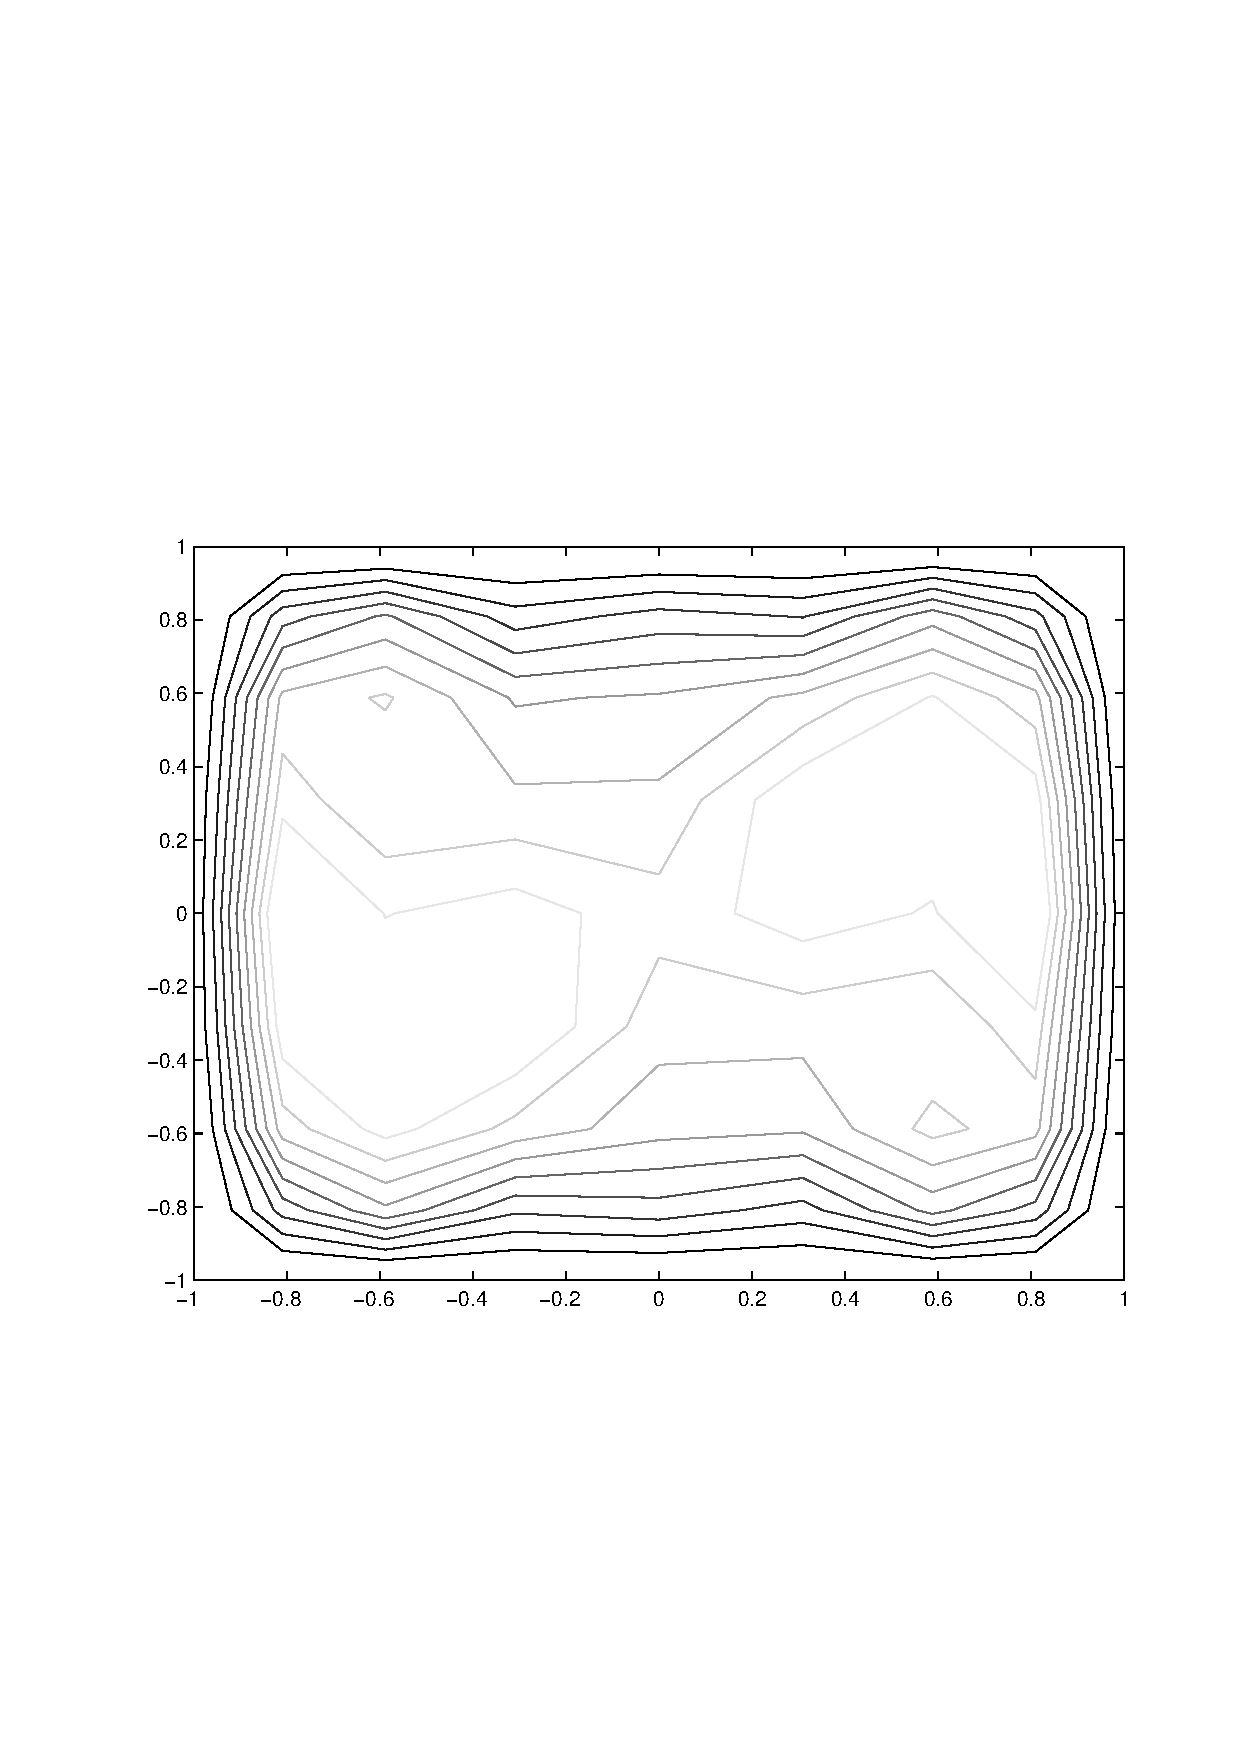
\includegraphics[scale=0.45, trim = 30mm 75mm 15mm 80mm, clip]{./Figures/4-IVBP/stream_t_8.pdf}
\caption{Stream function isolines, $t=0.8$.
}
\end{figure}


\columnbreak

\begin{figure}[H]
\centering
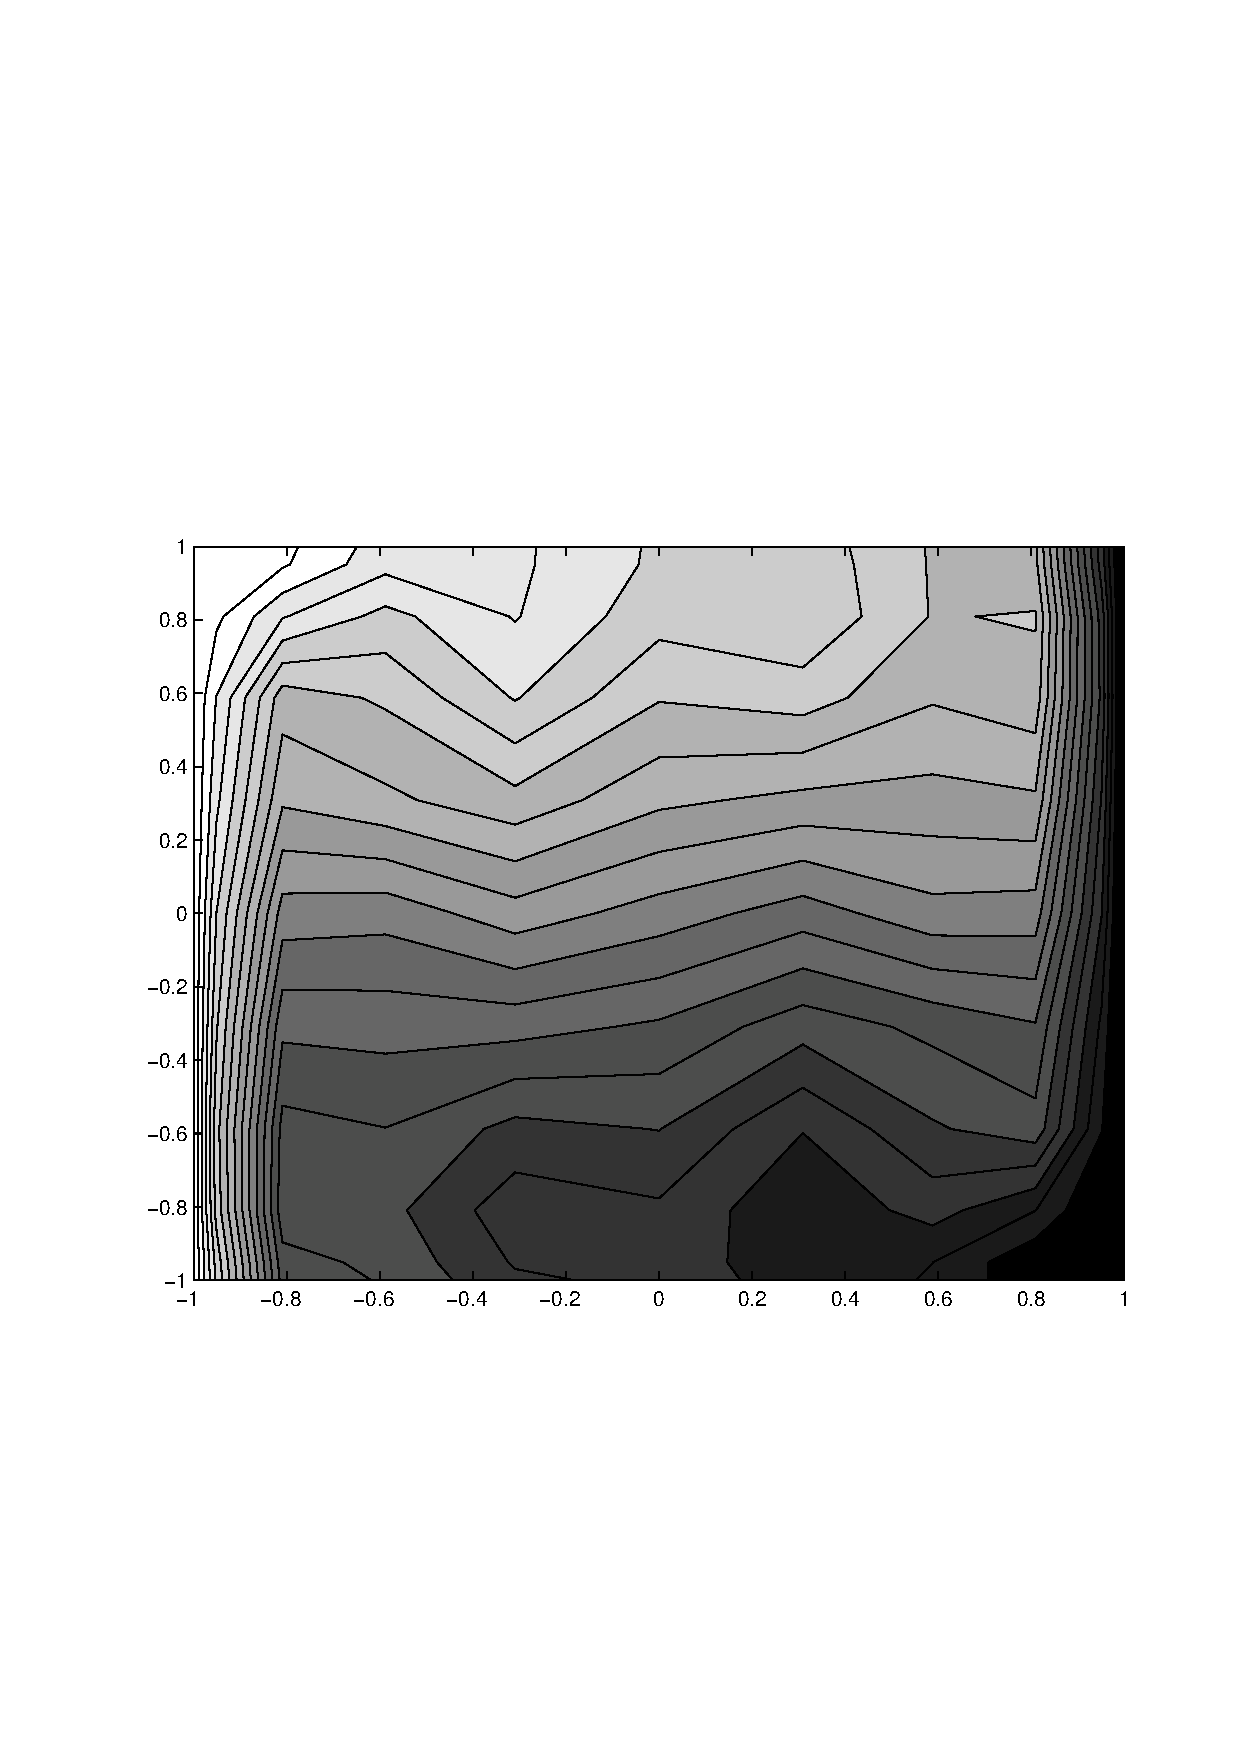
\includegraphics[scale=0.45, trim = 30mm 75mm 15mm 80mm,
clip]{./Figures/4-IVBP/temperature_t_8.pdf} \caption{Temperature contours, $t=0.8$.}
\end{figure}

\end{multicols}

\begin{multicols}{2}

\begin{figure}[H]
\centering
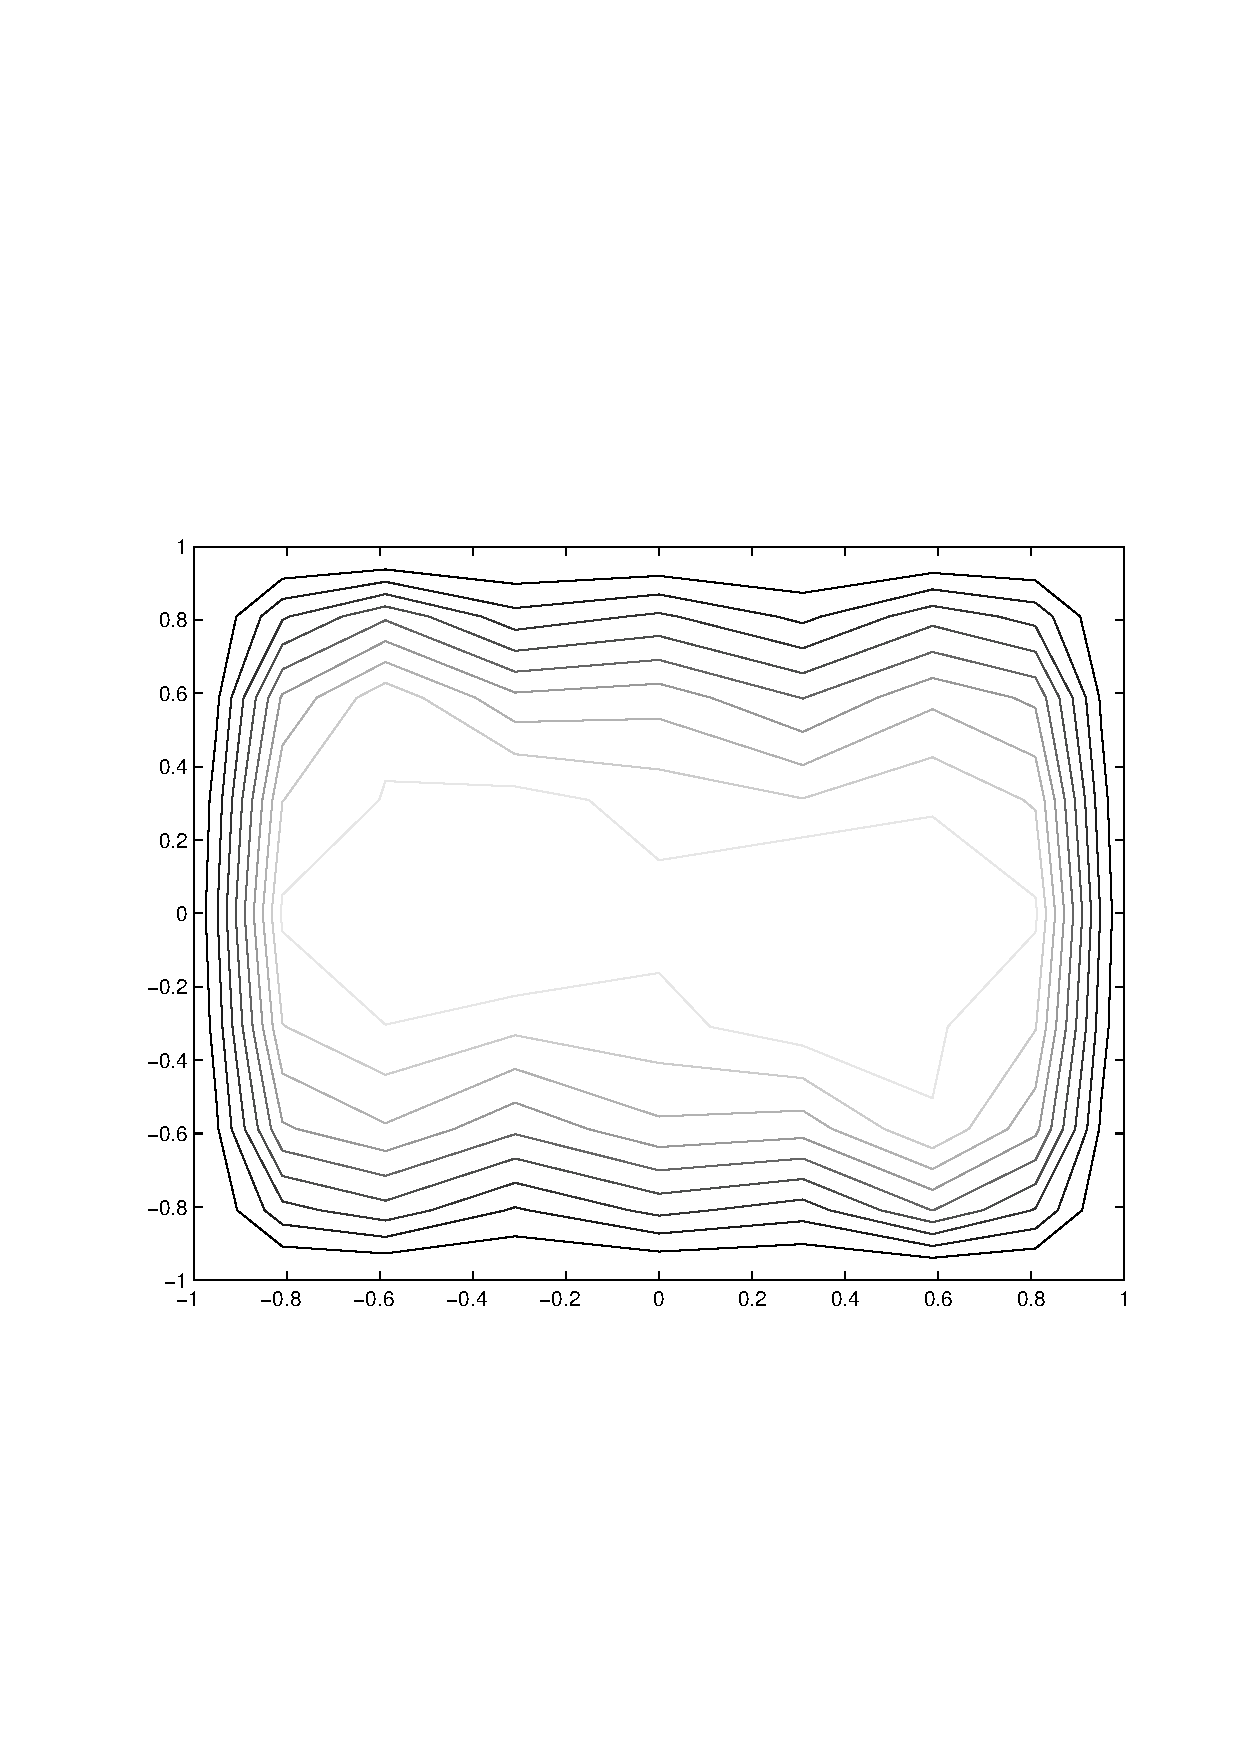
\includegraphics[scale=0.45, trim = 30mm 75mm 15mm 80mm, clip]{./Figures/4-IVBP/stream_t_10.pdf}
\caption{Stream function isolines, $t=1$.
}
\end{figure}


\columnbreak

\begin{figure}[H]
\centering
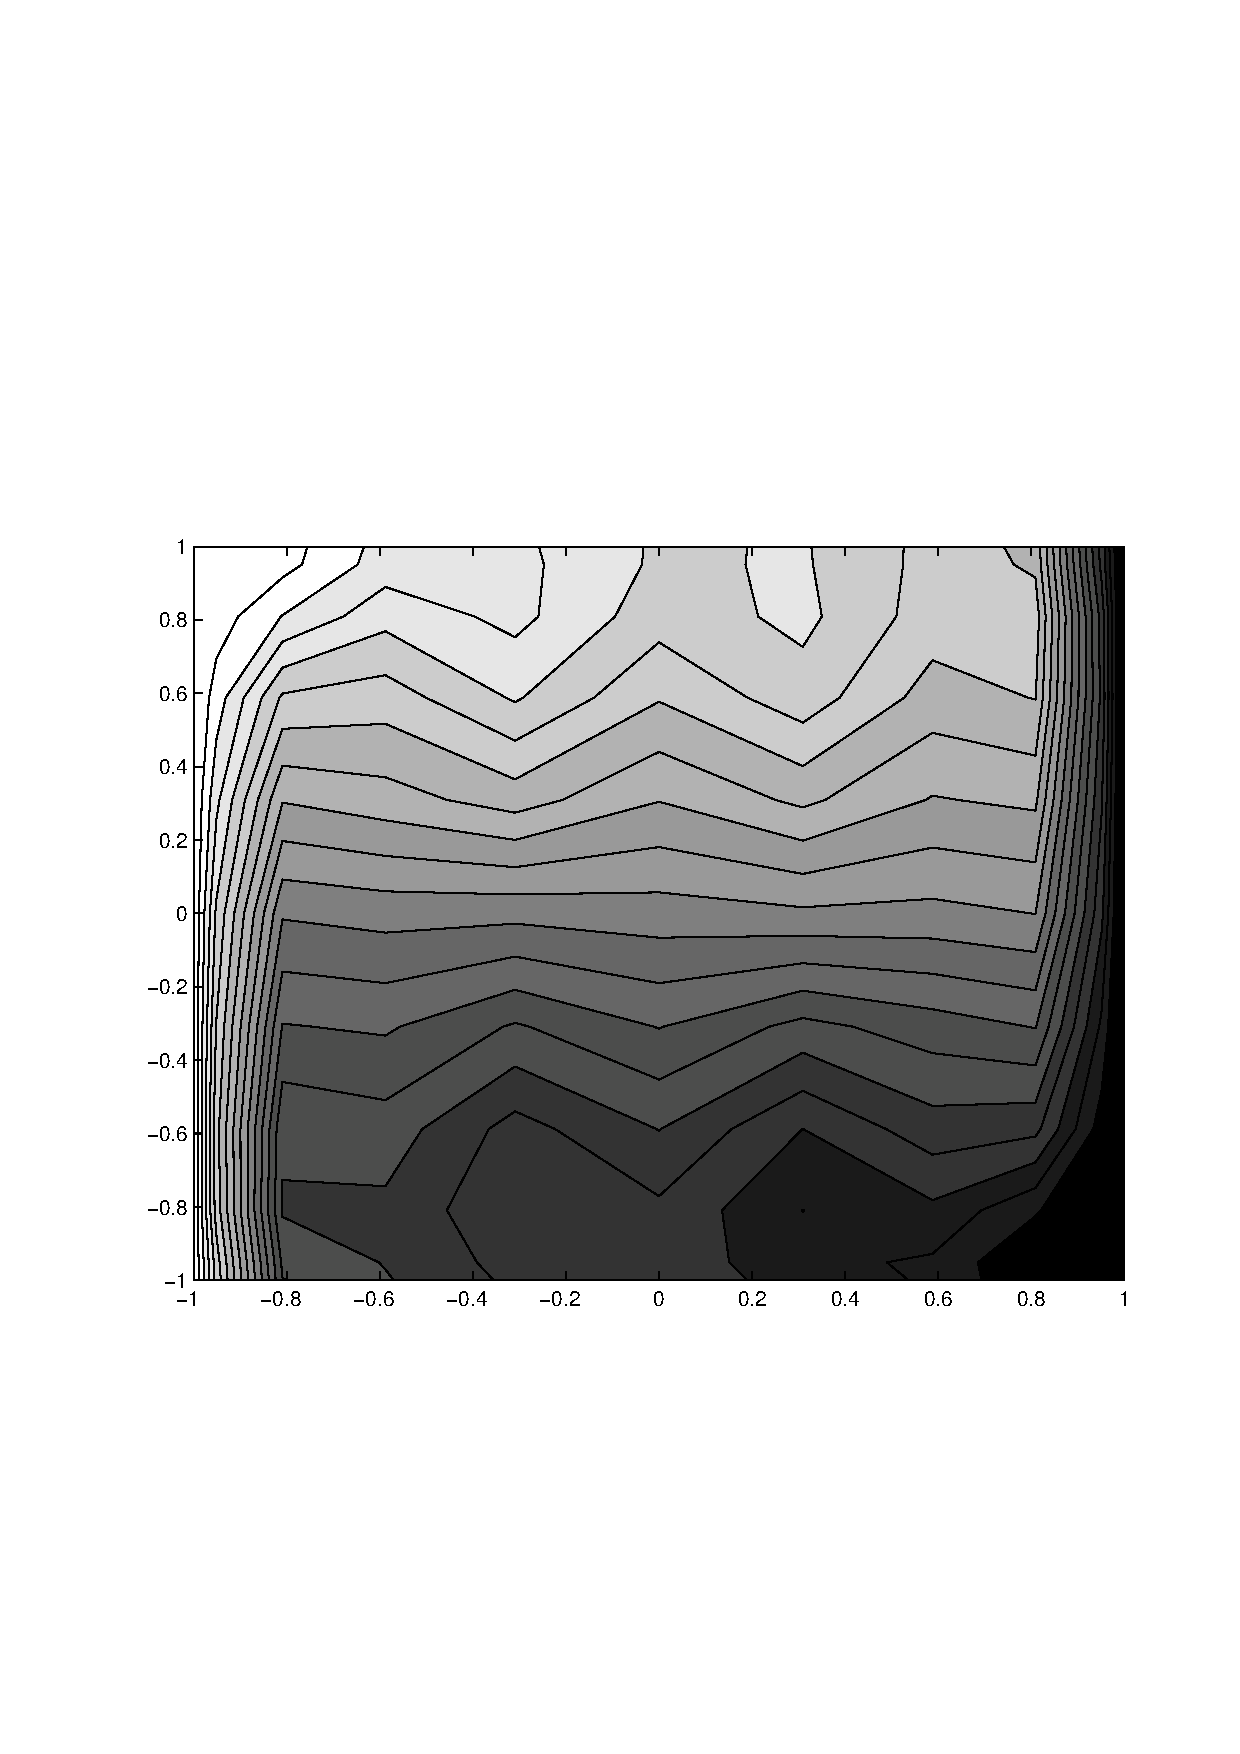
\includegraphics[scale=0.45, trim = 30mm 75mm 15mm 80mm,
clip]{./Figures/4-IVBP/temperature_t_10.pdf} \caption{Temperature contours, $t=1$.}
\end{figure}

\end{multicols}

\vspace{0.5cm}

\section{Convergence of the solution}

There are several techniques for evaluating the convergence of numerical
methods. Here we propose \textit{Richardson Extrapolation Method} for testing
our schemes. \\

\subsection{Richardson extrapolation}

This method is useful to test the convergence of the evolution problem. \\

One can assume that the exact solution (unknown) of the problem ($A$) can be
written as follows: 

\begin{equation}
A=A(h)+ K\cdot h^{\kappa} + K'\cdot h^{\kappa+1}+\ldots
\end{equation}

Where $A(h)$ is the numerical solution found when the time step is set to $h$;
and $\kappa$ is a parameter which depend on the temporal scheme used to solve
the problem ($\kappa=1$ with Euler's, Runge-Kutta:  $\kappa=4$). $K$ is
an unknown scalar.\\

One can also write: 

\begin{equation}
A=A(h)+ K\cdot h^{\kappa} + o(h^{\kappa+1})
\end{equation}

In order to evaluate the numerical convergence of the procedure, the program is
to be executed twice, with time steps set to $h$ and $h/2$. Two solutions are
obtained: $A(h)$ and $A(h/2)$: 

\begin{equation} \label{Richardson}
\begin{cases}
A=A(h)+ K\cdot h^{\kappa} + o(h^{\kappa+1})\\
A=A(h/2)+ K\cdot (h/2)^{\kappa} + o(h^{\kappa+1})
\end{cases}
\end{equation}

One can estimate the exact solution with these two equations: 

\begin{equation}
\begin{cases}
A=A(h)+ K\cdot h^{\kappa} + o(h^{\kappa+1})\\
2^{\kappa} \cdot A= 2^{\kappa}\cdot A(h/2)+ K\cdot (h)^{\kappa} +
o(h^{\kappa+1})
\end{cases}
\end{equation}

\begin{equation}
(2^{\kappa}-1) \cdot A= 2^{\kappa}\cdot A(h/2)- A(h) +
o(h^{\kappa+1})
\end{equation}

\begin{equation}
A= \frac{2^{\kappa}\cdot A(h/2)- A(h)}{(2^{\kappa}-1) } +
o(h^{\kappa+1})
\end{equation}

Then, the error for $h/2$ is: 

\begin{equation}
E(h/2) = A-A(h/2) = \frac{2^{\kappa}\cdot A(h/2)- A(h)}{(2^{\kappa}-1) } -
A(h/2)
\end{equation}

\begin{equation}
E(h/2) =  \frac{ A(h/2)- A(h)}{(2^{\kappa}-1) } 
\end{equation}

This easy procedure allows us to test the functioning of the numerical schemes
and the software application. Large errors indicate a strong dependence of the
solution with the time step, and the solution found is not trustable.\\

In the other hand, small errors give confidence to the method and the numerical
solution is more likely close to the exact solution.\\

As always, if we have an analytical solution, the goodness of the numerical
approach can be evaluated directly. \\

\newpage

If the error found does not satisfy our requirements a narrower time step
is required. It is easy to estimate the time step needed for a target error.
Going back to the equation \ref{Richardson}: 

\begin{equation}
A(h)-A(h/2)=-K\cdot (h^\kappa - (h/2)^\kappa)
\end{equation} 

\begin{equation}
K =-\frac{A(h)-A(h/2)}{ h^\kappa-(h/2)^\kappa }= \frac{A(h/2)-A(h)}{
h^\kappa \cdot(1-(1/2)^\kappa )}
\end{equation} \\

So the error can be calculated as follows,

\begin{equation}
E(h/2) = A-A(h/2) \simeq K(h/2)^\kappa+o(h^{\kappa+1})
\end{equation}

Then, 

\begin{equation}
E(h/2)  \simeq K(h/2)^\kappa
\end{equation}

With this equation we can set the time step to meet our requuirements. Let's
picture we want a precision lower than $1E-6$, then the time step needed is: 

\begin{equation}
h< 2 \cdot \left ( \frac{E(h/2)}{K}\right)^{1/\kappa}  
\end{equation}








\newpage
\chapter*{Conclusion and perspectives}
\addcontentsline{toc}{chapter}{\protect\numberline{}Conclusion and perspectives}



\newpage
\listoffigures
\addcontentsline{toc}{chapter}{List of figures}

\newpage
\printindex
\addcontentsline{toc}{chapter}{Index}









\end{document}
